\documentclass[11pt,a4paper]{article}
\usepackage{lmodern}
\usepackage[utf8]{inputenc}
\usepackage[french]{babel}
\usepackage[T1]{fontenc}
\usepackage{amsmath}
\usepackage{amsfonts}
\usepackage{amssymb}
\usepackage{graphicx}
\usepackage[hidelinks]{hyperref}
\usepackage[top=2.5cm, bottom=4.5cm, left=1.5cm, right=1.5cm]{geometry}
\usepackage{fancyhdr}
\usepackage[bottom]{footmisc} % footnote below figures
\usepackage{verbatim}
\usepackage{enumitem} % pimp les itemizes
%Pour mettre deux figures côtes à côtes
\usepackage{caption} 
\usepackage{subcaption}
% reference figure
\usepackage{hyperref}
%cropping figures
\usepackage{adjustbox}
\usepackage{setspace} %spacing
\usepackage{ulem} % \ul
% \usepackage{algorithm2e} % pseudo code
% \usepackage{siunitx}
\usepackage{multirow} % pour des tableaux multicolumns
% \usepackage{float} 

\usepackage[titletoc,page]{appendix}
% \usepackage{chngcntr}
% \counterwithout{figure}{section}

% \setlength\parindent{0pt} % Removes all indentation from paragraphs

\usepackage{xcolor}
\definecolor{Mgray}{RGB}{240,240,240}
\usepackage{listings} % for code
\usepackage{courier} % change the font
\lstset{
    basicstyle=\footnotesize\ttfamily, % Default font
    numbers=left,              % Location of line numbers
    numberstyle=\tiny,          % Style of line numbers
    % stepnumber=2,              % Margin between line numbers
    numbersep=5pt,              % Margin between line numbers and text
    tabsize=2,                  % Size of tabs
    extendedchars=true,
    breaklines=true,            % Lines will be wrapped
    keywordstyle=\color{red},
    frame=lrtb,
    stringstyle=\color{white}\ttfamily, % Color of strings
    showspaces=false,
    showtabs=false,
    xleftmargin=17pt,
    framextopmargin = 3pt,
    framexleftmargin=17pt,
    framexrightmargin=5pt,
    framexbottommargin=4pt,
    %backgroundcolor=\color{lightgray},
    showstringspaces=false
}


%%%%%%%%%%%%%%%%%%%%%%%%%%%%%%%%%
%%        HEADER/FOOTER        %%
%%%%%%%%%%%%%%%%%%%%%%%%%%%%%%%%%

% redefine a style, here it is plain
\fancypagestyle{fancy}{ 
\fancyhf{}
\fancyfoot[RO, LE] {\thepage}
\fancyhead[RO] {\leftmark}
\fancyhead[LE] {\rightmark}
}
%\pagestyle{fancy}
%\newcommand{\question}[2]{\vspace{2em} \textbf{Question #1)} #2 \vspace{1em}}

% thanks https://tex.stackexchange.com/questions/114321/extensible-vec-instead-of-overrightarrow 

\newcommand{\xvec}[1]{\overrightarrow{#1}}
\newcommand{\zer}{\vspace{1em}}
\newcommand{\uncinq}{\texttt{1.5.2\_rev\_1900}}
\newcommand{\unsept}{\texttt{1.7.0\_stab\_1926}}

\title{Note de Stage\\Observatoire de Meudon} 
\author{Antoine Nasser}
\date{Printemps Été (chaud) 2019}

%%%%%%%%%%%%%%%%%%%%%%%%%%%
%%        Chapitre        %%
%%%%%%%%%%%%%%%%%%%%%%%%%%
% \renewcommand\partname{}
% \renewcommand{\thepart}{\Roman{part}) }
\renewcommand{\thesection}{\Roman{section}) }
\renewcommand{\thesubsection}{\Roman{section}-\arabic{subsection}) }
\renewcommand{\thesubsubsection}{\Roman{section}-\arabic{subsection}-\alph{subsubsection})}

%%%%%%%%%%%%%%%%%%%%%%
%%        GO        %%
%%%%%%%%%%%%%%%%%%%%%%

\begin{document}

\begin{spacing}{0.98}


\maketitle
\begin{center}{\Large Etude des processus de chauffage et de refroidissement \\ dans les régions de photodissociation (PDR)}\end{center}


\setcounter{secnumdepth}{4}
\vfill
\begin{figure*}[!hb]
        \centering 
        
\includegraphics[trim = {0 0 0 0cm},clip,width=0.8\textwidth]{figure/LERMA2.jpg}
\end{figure*}
\vfill

\tableofcontents

\setcounter{figure}{0}    

\newpage
 
\section*{Introduction}
%%%%%%%%%%%%%%%%%%%%%%%%%%%%%%%%%%%%%%%%%%%%%%%%%%%%%%%%%%%%%%%%%%%%%%%%%%%%%%%%%%%%%%%%%%%%%%%%%%%%%%%%





\section{Amplification de l'effet photoelectrique par le chlore}

\subsection{Neufeld and Wolfire}
\subsubsection{Profil des espèces dérivés du chlore}

Les réseaux d'astrochimie de PDR ont tendance à négliger le chlore qui a une abondance mineure dans les nuages. Or des espèces dérivées du chlore ont été observées en absorption dans des nuages diffus ($n \sim 10^2\ cm^{-3}$). Des raies de $\mathrm{H}_2\mathrm{Cl}^+$,HCl et $\mathrm{HCl}^+$ excitées ont également été observées par Herschel dans plusieurs sources de la Galaxie et notamment dans le nuage moléculaire de la barre d'Orion \cite{Neufeld2012,Neufire2009}. On a tout d'abord cherché à reproduire les résultats de \cite{Neufeld2009} en calculant les profils de densités à travers le nuage.

\begin{figure}[htbp]
    \centering
    \begin{subfigure}[t]{0.45\textwidth} % "0.45" donne ici la largeur de l'image
        \centering 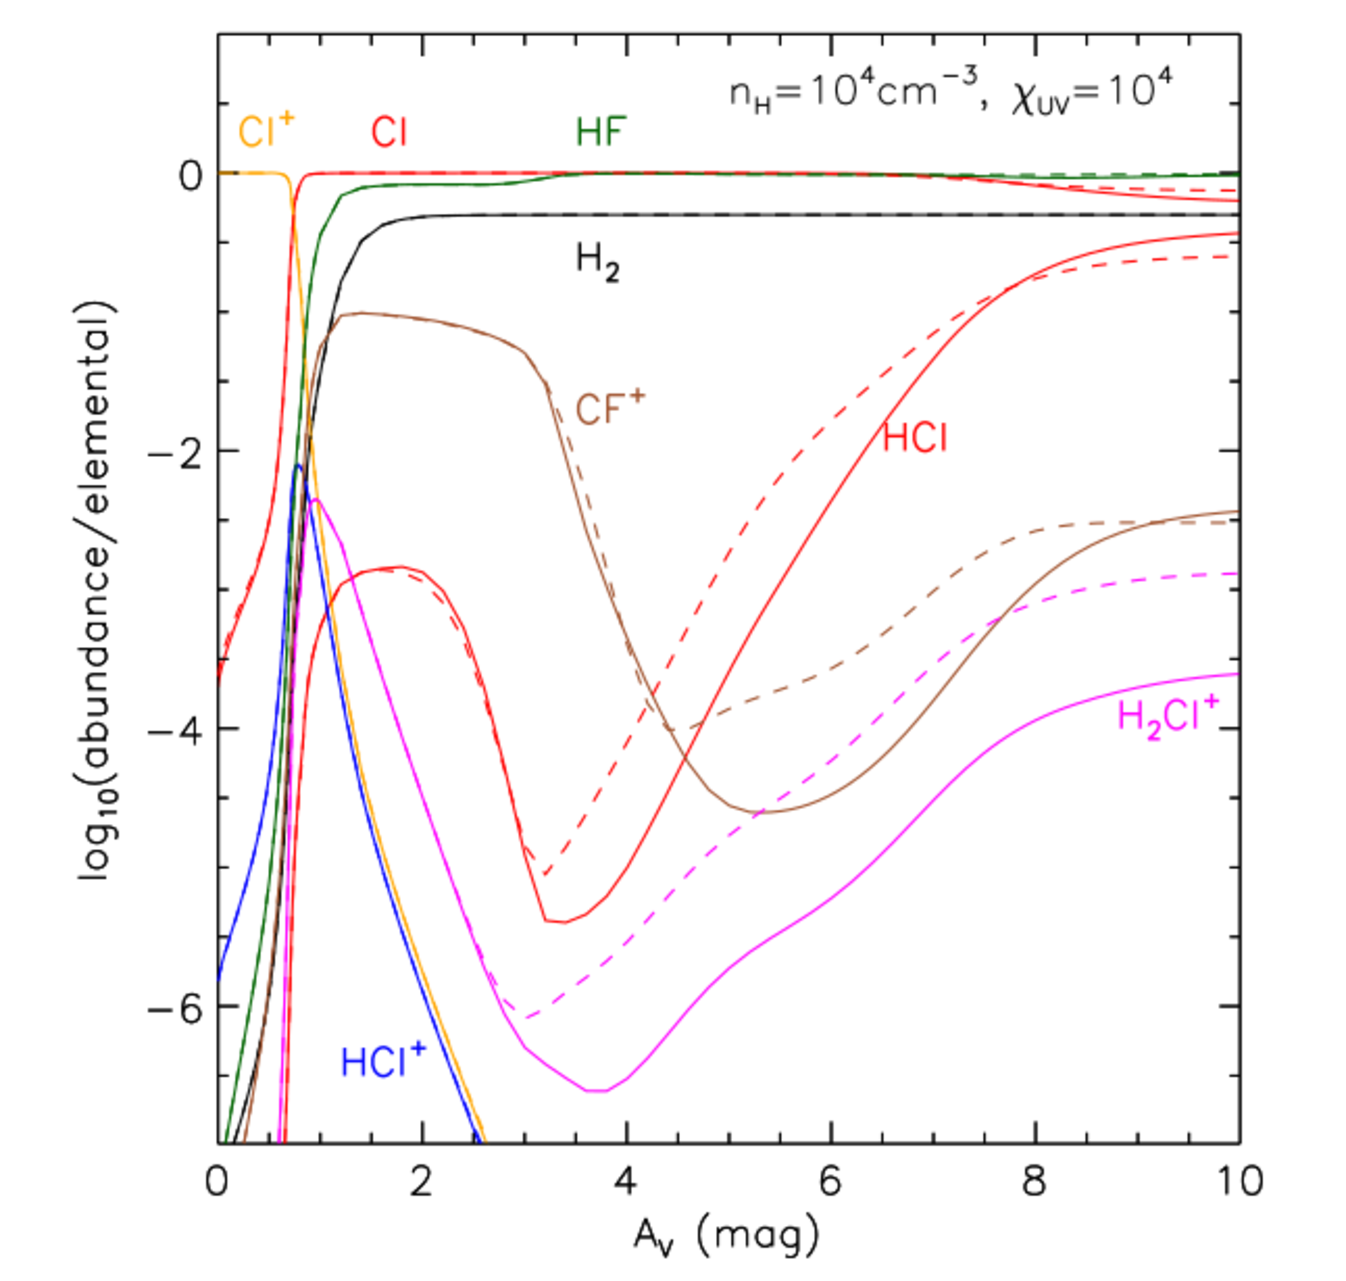
\includegraphics[trim = {0 0 0 0cm},clip,width=1\textwidth]{figure/Cl/neufire/dens.pdf}
        \caption{}
    \end{subfigure}
    ~ 
    \begin{subfigure}[t]{0.45\textwidth}
        \centering 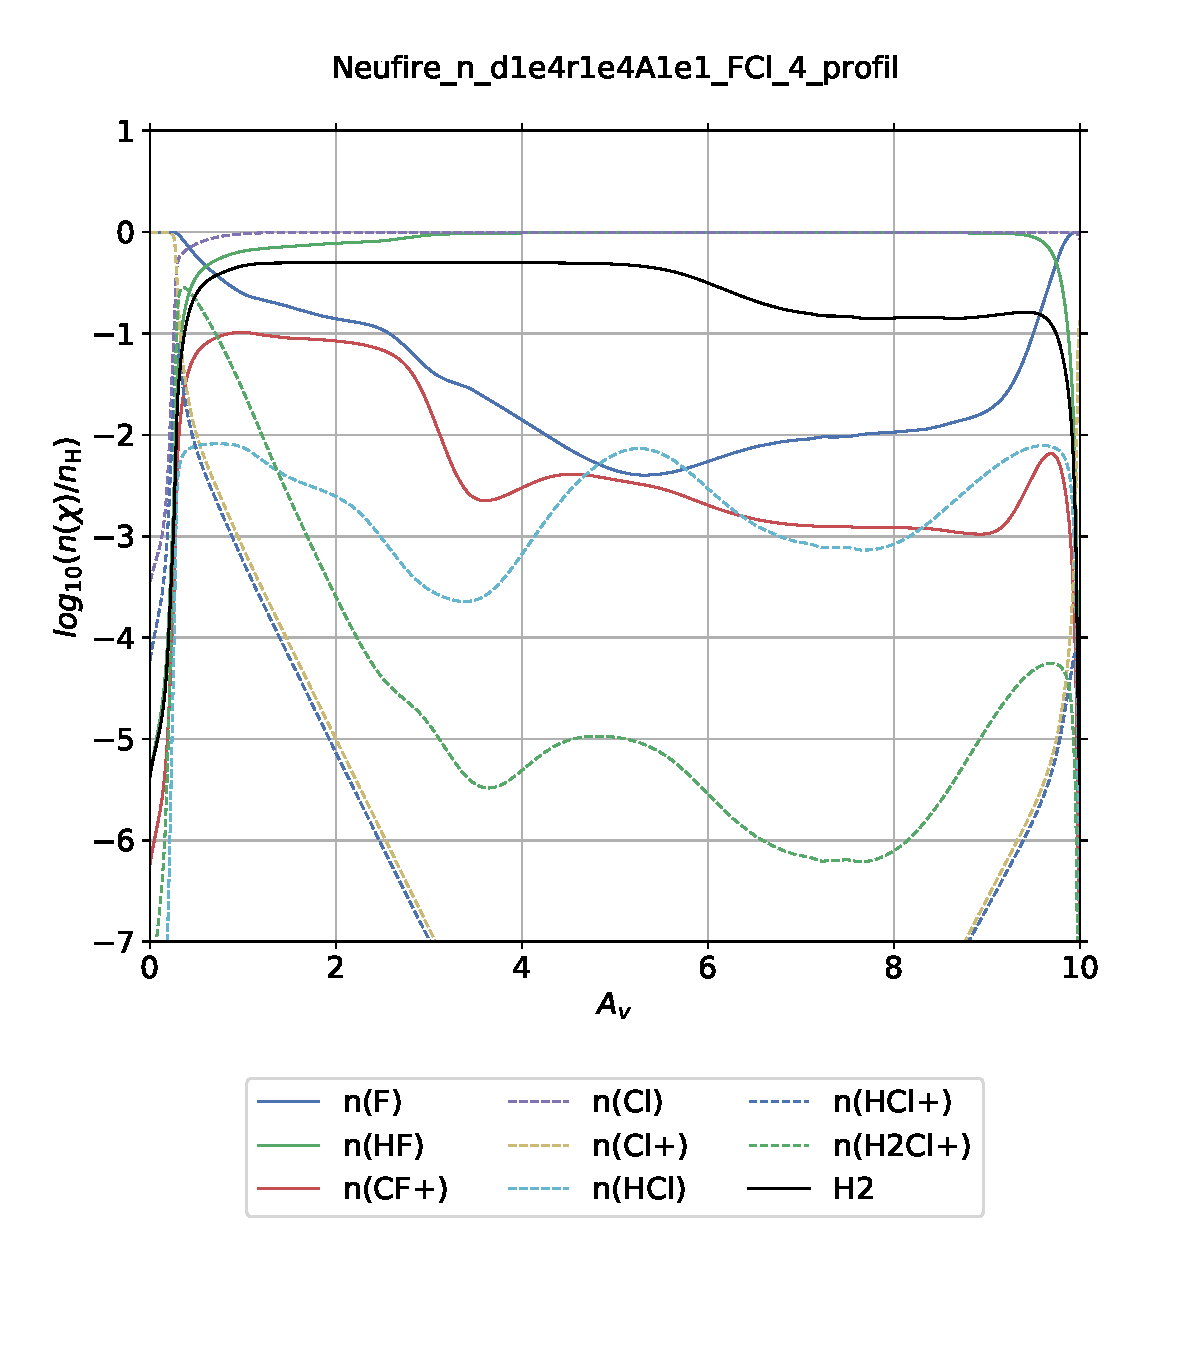
\includegraphics[trim = {0 2cm 0 1.8cm},clip,width=1\textwidth]{figure/Cl/neufire/HCl_profil.pdf}
        \caption{}
    \end{subfigure}
    \caption{Profil de densité pour un modèle isochore $n_\mathrm{H} = 10^4 \mathrm{cm}^{-3}$ et $\chi_\mathrm{UV} = 10^4$. La figure de gauche (a) est extraite de \cite{Neufire2009} où les profils sont obtenus à partir d'une version modifié du code de \cite{Kaufman2006}. Le trait plein est un calcul avec un taux de ionisation par les rayons cosmiques de $1.8 \times 10^{−17 } \mathrm{s}^{-1}$ par atome d'hydrogène, tandis qu'en pointillé $1.8 \times 10^{−16} \mathrm{s}^{-1}$ . A droite (b) le code PDR de Meudon résout la PDR en utilisant le même réseau chimique proposé dans \cite{Neufire2009}.}
\end{figure}

Pour valider le réseau chimique implanté dans le code on a imposé au code de Meudon de suivre le profil de température donné dans l'article. On a également supprimé la formation du $\mathrm{H}_2$ sur les grains en utilisant une réaction équivalente permettant sa formation dans le nuage moléculaire qui ne serait pas possible dans un modèle isochore. On voit que l'on retrouve les allures des profils de densités. Les profils du $\mathrm{Cl}$,$\mathrm{Cl}^+$, $\mathrm{HCl}$, $\mathrm{HF}$ sont proches en ordre de grandeurs. Ceux du $\mathrm{H}_2\mathrm{HF}^+$, $\mathrm{HCl}^+$, $\mathrm{CF}^+$ n'ont pas exactement les mêmes allures ni les mêmes valeurs. 

\subsubsection{Existence d'une branche haute température}

Si l'on laisse le code résoudre la température, on voit qu'en fin de zone atomique le nuage chauffe brusquement suggérant qu'il y a deux solutions possibles en cette région du nuage et que le code a sauté sur une des deux solutions...

\begin{figure}[htbp]
    \centering
    \begin{subfigure}[t]{0.45\textwidth} 
        \centering 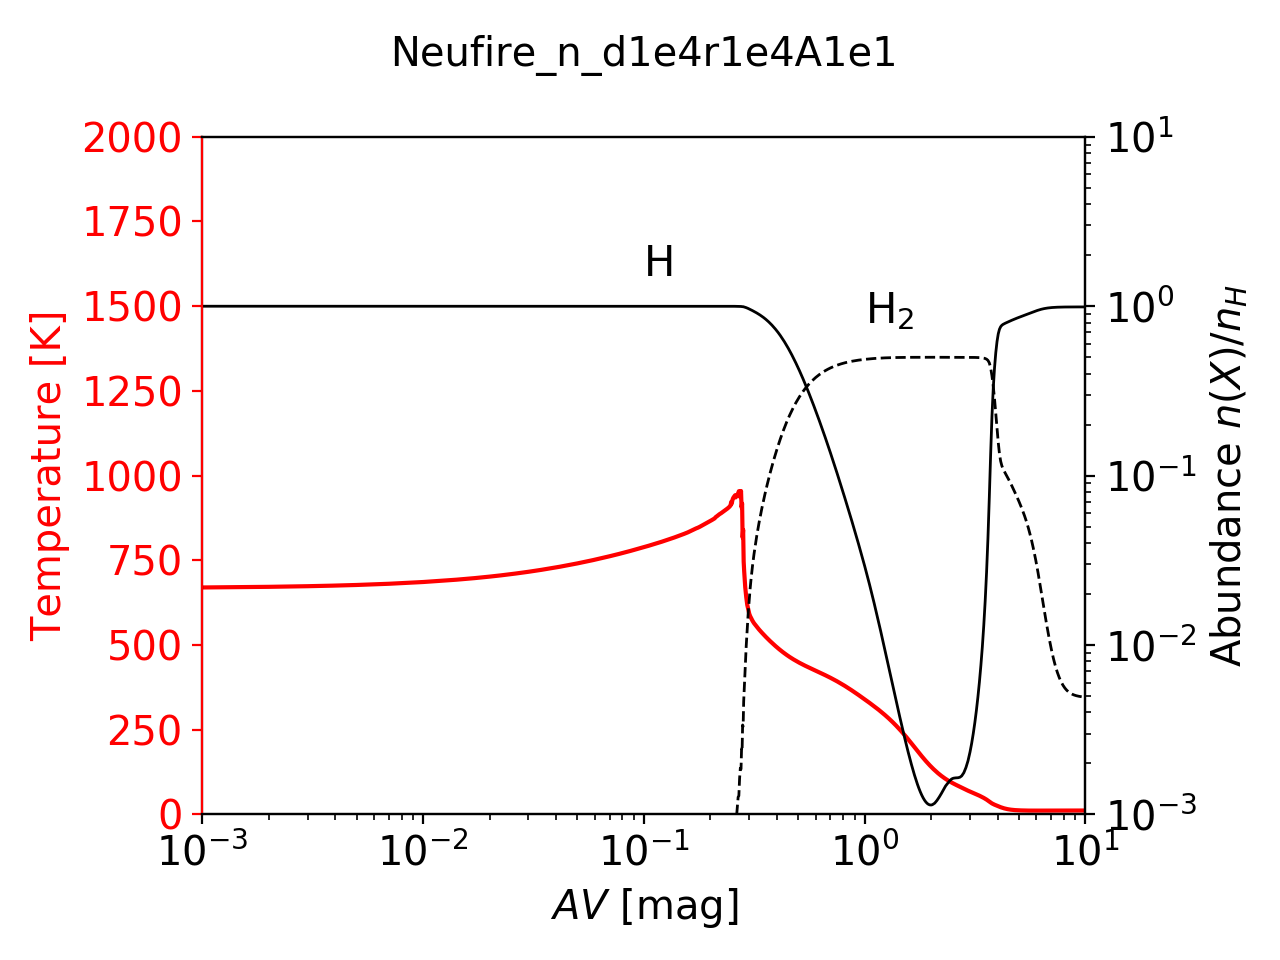
\includegraphics[trim = {0 0 0 1cm},clip,width=1\textwidth]{figure/Cl/neufire/profil_H_noCl.png}
        \caption{Sans chlore}
    \end{subfigure}
    ~ 
    \begin{subfigure}[t]{0.45\textwidth}
        \centering 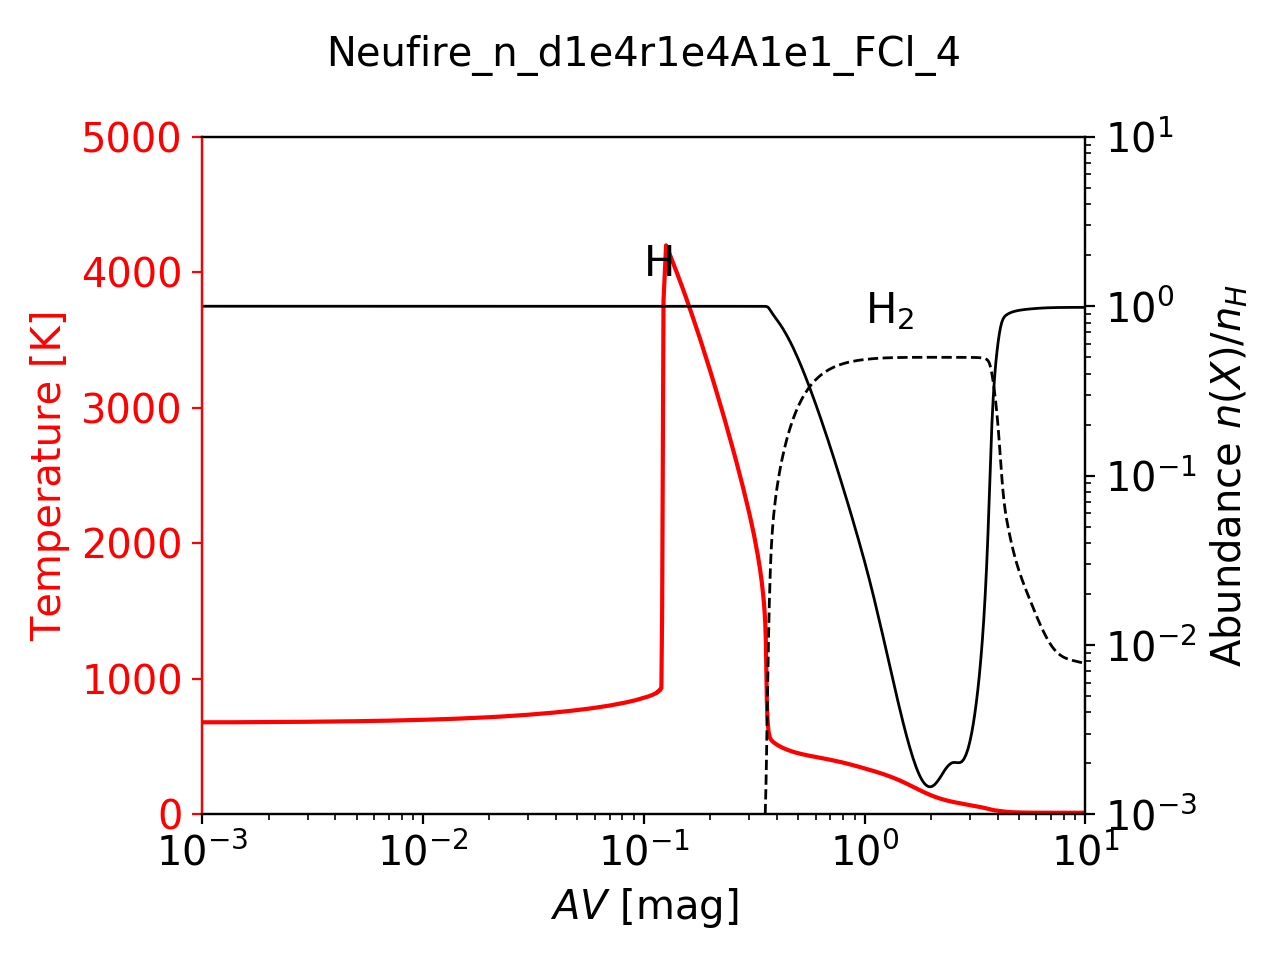
\includegraphics[trim = {0 0cm 0 1cm},clip,width=1\textwidth]{figure/Cl/neufire/profil_H.png}
        \caption{Avec chlore}
    \end{subfigure}
    \caption{}
\end{figure}



\subsection{Analyse du rôle du chlore}

\begin{figure}[htbp]
    \centering
    \begin{subfigure}[t]{0.45\textwidth} % "0.45" donne ici la largeur de l'image
        \centering \includegraphics[trim = {0 0 0 1cm},clip,width=1\textwidth]{figure/model_Cl/PDR155_n_d1e5r1e4A2e1.png}
        \caption{Profil de température et densité en fonction de la profondeur dans le nuage}\label{fig:ClT}
    \end{subfigure}
    ~ 
    \begin{subfigure}[t]{0.45\textwidth}
        \centering \includegraphics[trim = {0 0 0 1cm},clip,width=1\textwidth]{figure/model_Cl/tb_PDR155_n_d1e5r1e4A2e1.png}
        \caption{Taux de chauffage et refroidissement en fonction de la température du gaz au bord atomique du nuage ($A_{\mathrm{V}} = 10^{-6}$)}\label{fig:ClHC}
    \end{subfigure}
    \caption{Profil de densité de l'hydrogène et de la température en fonction de l'extinction dans le visible.}
\end{figure}

J'ai étudié les réactions chimiques principales qui se déroulent en bord de nuage atomique et démontré que le chlore joue le rôle de catalyseur de l'effet photoélectrique. Le mécanisme est illustré sur la \autoref{fig:catalyseur}.
Le champs de rayonnement UV, intense en bord de nuage atomique, photoionise le chlore et produit des ions $\mathrm{Cl}^+$ et des électrons. Le transfert de charge du $\mathrm{Cl}^+$ avec l'hydrogène est une réaction rapide qui permet au chlore de se rendre de nouveau disponible pour la photoionisation. Le chlore permet ainsi de ioniser indirectement l'hydrogène. Par conséquent, la fraction électronique du gaz augmente.  
Or on sait que l'effet photoélectrique sur les grains fonctionne d'autant plus que la fraction électronique dans le nuage est importante \footnote{Une forte densité d'électrons rend plus facile la recombinaison électronique des grains ce qui maintient le degré d'ionisation des grains raisonnablement faible. Il est plus facile d'arracher un électron d'un grain neutre que d'un grain qui a déjà été ionisé.}. 
L'effet photoélectrique chauffe ainsi le gaz ce qui améliore l'efficacité du transfert de charge du $\mathrm{Cl}^+$ avec l'hydrogène. 
En d'autres termes, le chlore induit une rétroaction positive de l'effet photoélectrique sur les grains. Cet emballement a tendance à chauffer le gaz à des températures nettement plus fortes et ce malgré la faible abondance du chlore. \newline

\begin{figure}[b!]
   \centering
        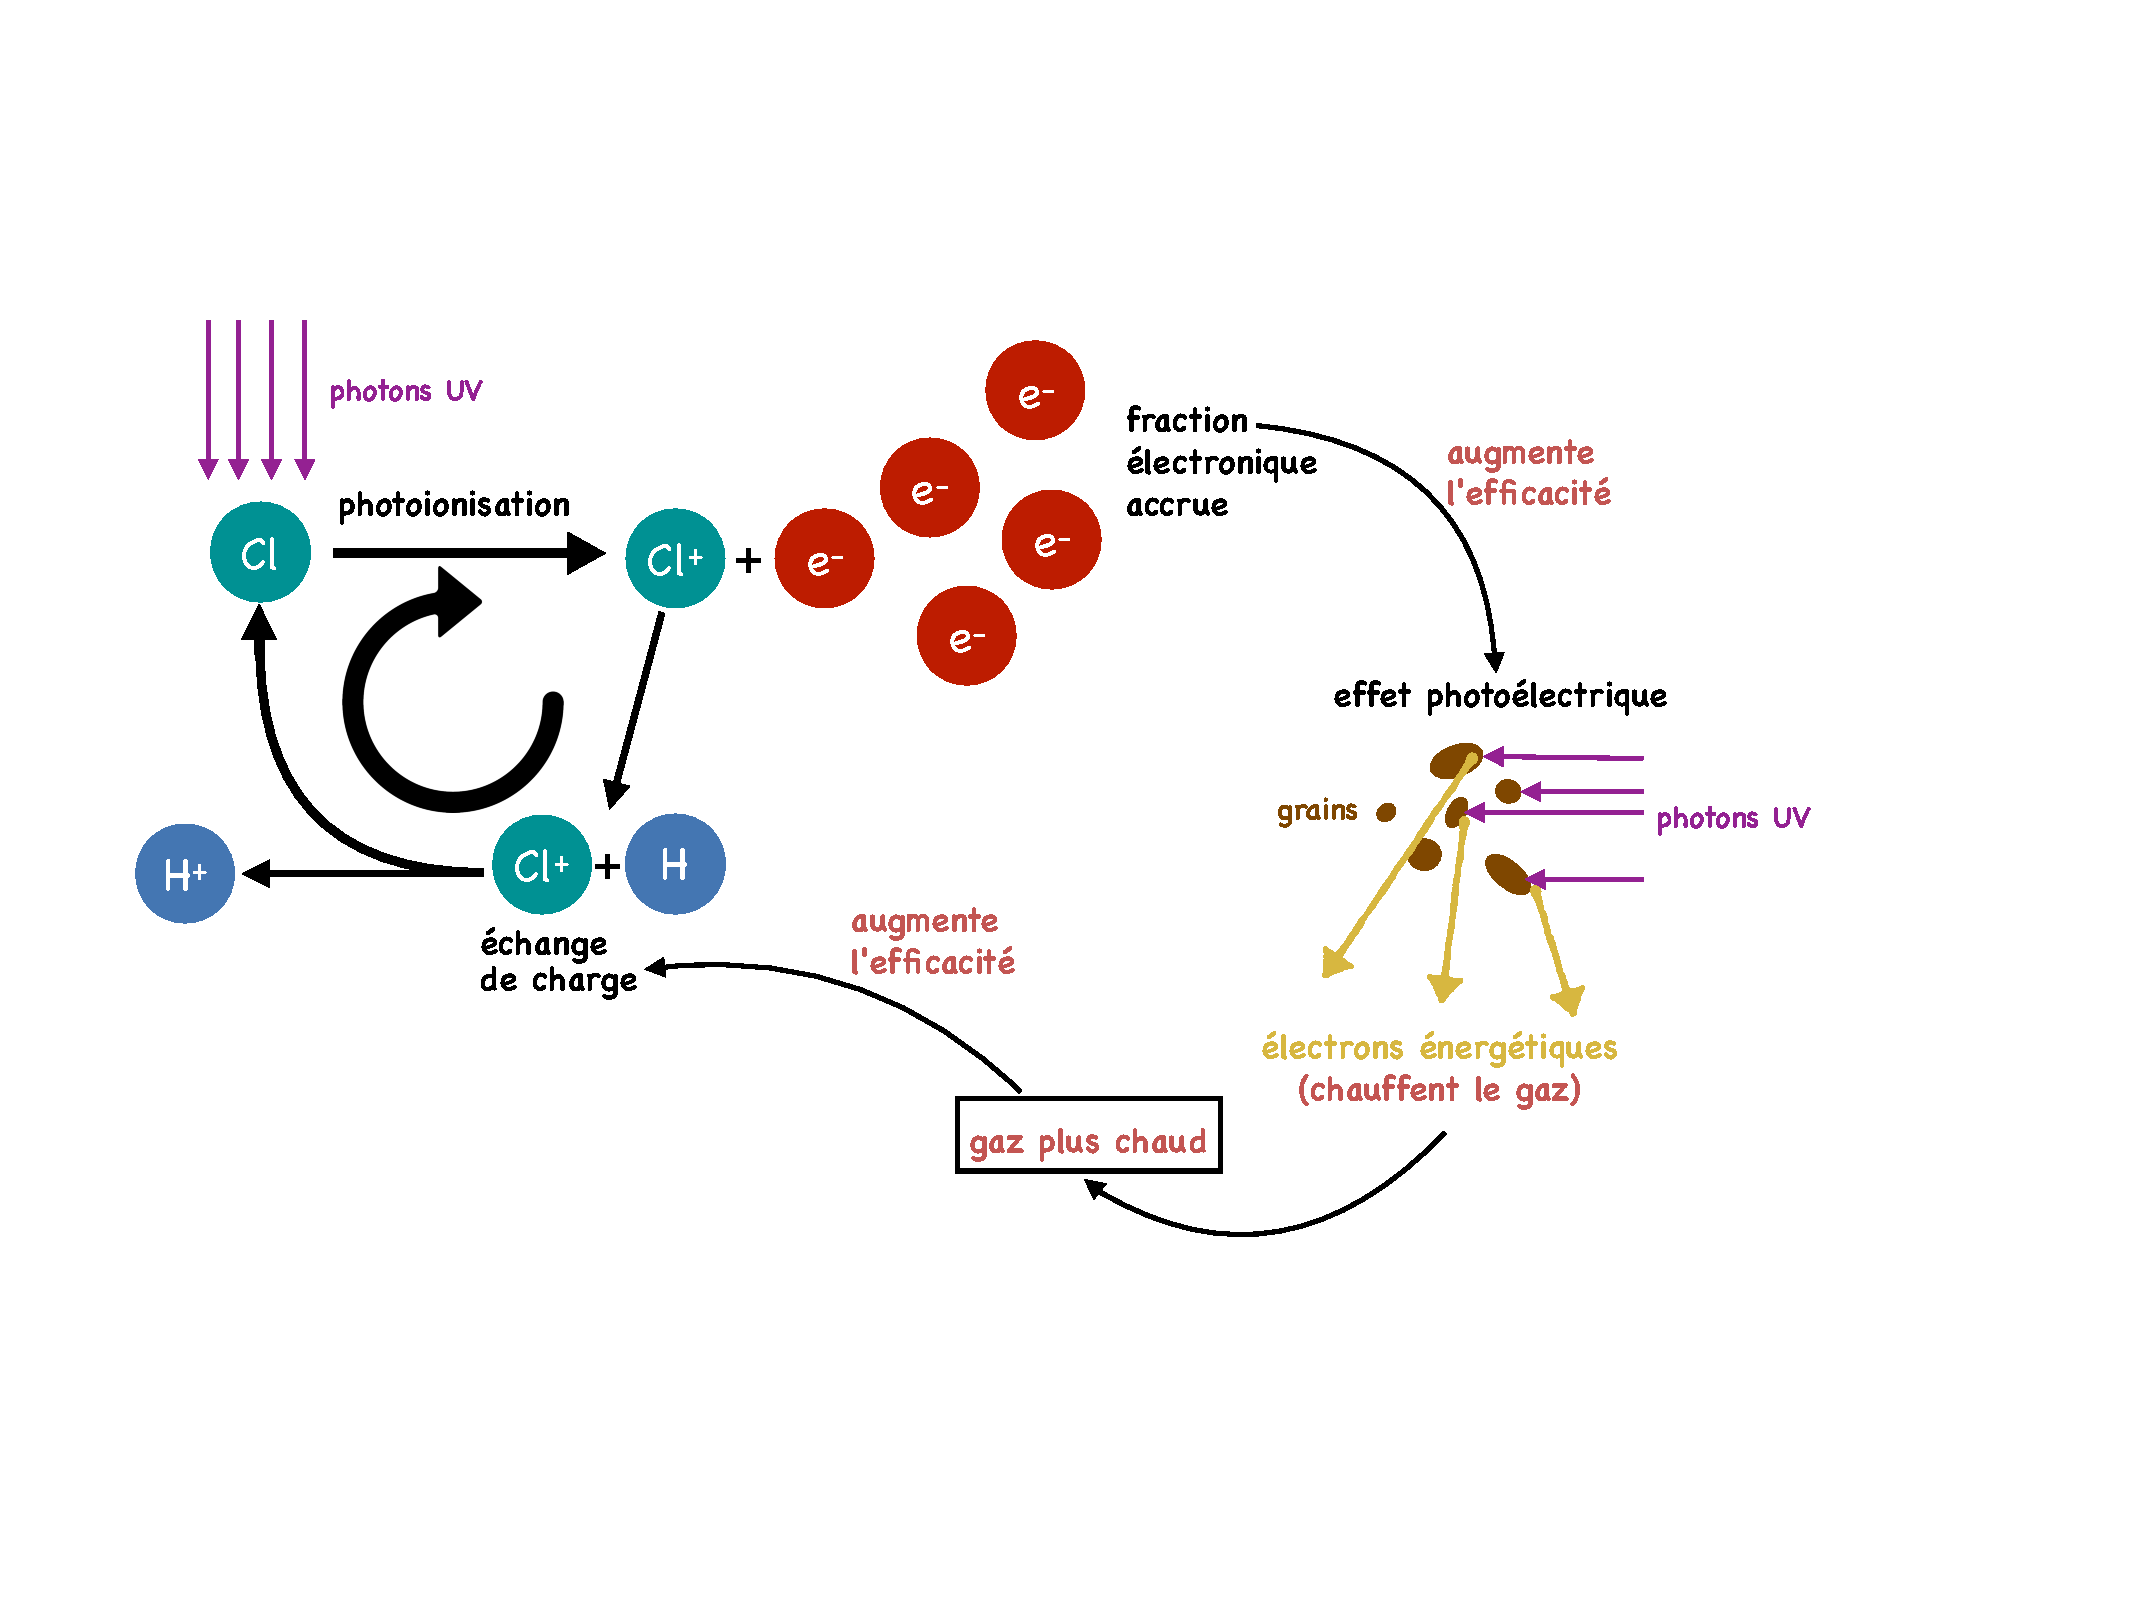
\includegraphics[trim = {2cm 5cm 4cm 4cm},clip, width=0.8\textwidth]{figure/Cl/Cl_heating_fr-5.pdf}
    \caption{Schéma représentant l'impact du chlore sur la chimie de bord de nuage atomique}
    \label{fig:catalyseur}
\end{figure}{}

L'emballement de l'effet photoélectrique se produit à partir de 1000 K. Or la photoionisation du carbone et du soufre produit les électrons en bord de nuage atomique indépendamment de la température. Il existe une température où le transfert de charge devient suffisamment efficace pour que la fraction d'électrons créée via le chlore devienne dominante devant celle de la ionisation du carbone et du soufre et amorce la rétroaction de l'effet photoélectrique. L'amplification dépend donc l'énergie d'activation du transfert de charge $\mathrm{Cl}^+  + \mathrm{H}    \rightarrow \mathrm{Cl}   +  \mathrm{H}^+$ qui vaut 6290 K. \newline

Parmi les espèces figurant dans le modèle, la carbone, le soufre, le silicium ou le fer ont également un potentiel de ionisation inférieur à celui de l'hydrogène (\autoref{tab:gaz}). Pourtant aucun ne peut effectuer un transfert de charge avec l'hydrogène qui est l'espèce majoritaire en bord de nuage atomique. Ces espèces ne peuvent pas donc pas provoquer un emballement similaire à celui induit par le chlore. 



%%%%%%%%%%%%%%%%%%%%%%%%%%%%%%%%%%%%%%%%%%%%%%%%%%%%%%%%%%%%%%%%%%%%%%%%%%%%%%%%%%%%%%%%%%%%%%%

\subsection{Modèle analytique - Chimie}

Les espèces qui contribuent à la production d'électrons en bord de nuage sont les ions hydrogènes $\mathrm{H}^+$, carbones $\mathrm{C}^+$ et soufres $\mathrm{S}^+$. On peut supposer qu'en entrée de nuage atomique le carbone et le soufre sont ionisés ce qui fournit une fraction d'électrons minimale de $10^{-4}$. Le modèle doit retrouver l'augmentation de la densité d'électrons (jusqu'à $2\ 10^{-3}$) pour des températures supérieures à 1000 K.
 
\subsubsection{Ion hydrogène}

J'ai isolé les réactions principales qui font intervenir les ions $\mathrm{H}^+$. Les réactions avec l'oxygène sont négligées car la formation et destruction de $\mathrm{H}^+$ par l'oxygène se compensent totalement en première approximation. 

\begin{equation}
    \begin{array}{lccccclr}
        \mathrm{Cl}^+ & + &\mathrm{H}   & \rightarrow &\mathrm{Cl}  & + & \mathrm{H}^+ & (k_3) \\
        \mathrm{Cl}  & + & \mathrm{H}^+  & \rightarrow & \mathrm{Cl}^+ & + &\mathrm{H}  & (k_4) \\
        \mathrm{H}^+  & + & \mathrm{e}^-  & \rightarrow &\mathrm{H}   &   &     & (k_5) \\
    \end{array}
\end{equation}

A l'état stationnaire, le bilan de formation des ions $\mathrm{H}^+$ donne
\begin{equation}\label{eq:h+}
    \frac{d}{dt}n(\mathrm{H}^+) = k_3n(\mathrm{Cl}^+)n(\mathrm{H}) - k_4n(\mathrm{Cl})n(\mathrm{H}^+) - k_5 n(\mathrm{H}^+)n(\mathrm{e}^-) = 0
\end{equation}

En introduisant la fraction atomique de chlore $\delta_{Cl}$, fixée dans le gaz, et le bilan de charge on obtient une équation en $n(\mathrm{H}^+)$ :

\begin{equation}
    -k_3n(\mathrm{Cl}^+)n_{\mathrm{H}} + \bigg( \frac{k_3 k_4}{k_1} n_{\mathrm{H}} n(\mathrm{Cl}^+) + k_5 \big(n(\mathrm{C}^+)+ n(\mathrm{S}^+)\big) \bigg) n(\mathrm{H}^+) + k_5 n(\mathrm{H}^+)^2 = 0
\end{equation}

 avec,
\begin{equation}
    \delta_{Cl} = \SI{1.8}{10^{-7}} = \frac{n(\mathrm{Cl}) + n(\mathrm{Cl}^+) + ...}{n(\mathrm{H}) + n(\mathrm{H}^+) + 2n(\mathrm{H}_2) + ...} \approx \frac{1}{n_{\mathrm{H}}} (n(\mathrm{Cl}) + n(\mathrm{Cl}^+) )
\end{equation}

On obtient une solution qui dépend de $n(\mathrm{Cl}^+)$,
\begin{equation}
\resizebox{1.1\hsize}{!}{
    \boxed{n(\mathrm{H}^+) = -\frac{1}{2} \bigg( \frac{k_3 k_4}{k_1 k_5} n_{\mathrm{H}} n(\mathrm{Cl}^+) + n(\mathrm{C}^+)+ n(\mathrm{S}^+) \bigg) \pm \frac{1}{2} \sqrt{\bigg( \frac{k_3 k_4}{k_1 k_5} n_{\mathrm{H}} n(\mathrm{Cl}^+) + n(\mathrm{C}^+)+ n(\mathrm{S}^+) \bigg)^2 + 4\frac{k_3}{k_5}n_{\mathrm{H}} n(\mathrm{Cl}^+)}}
    }
\end{equation}

% \subsubsection{Rôle de l'oxygène}
% Au vu des taux de réactions impliquant le $\mathrm{H}^+$ nous pourrions choisir d'inclure la chimie de $\mathrm{H}^+$ avec l'oxygène. A hautes températures, les taux de $ \mathrm{H}^+ + O \leftrightarrows\mathrm{H}+ O^+ \quad (k_6,k_7)$ prédominent sur les autres réactions. Si l'on considère que ces réactions pour la chimie de l'oxygène, les $\mathrm{H}^+$ produits seront consommés pour former du $H$. Rien ne se passe. Pour s'en convaincre il suffit d'écrire la nouvelle équation bilan de $\mathrm{H}^+$ et d'utiliser celle pour $O^+$.

% \begin{equation}
%     \frac{d}{dt}n(O^+) = k_6 n(\mathrm{H}^+)n(O) - k_7n(\mathrm{H})n(O^+) = 0
% \end{equation}

% En l'injectant dans le nouveau bilan de formation pour le $\mathrm{H}^+$, ces nouveaux termes disparaissent. Cependant si l'on calcule l'expression de $n(\mathrm{H}^+)$ à partir des concentrations de $n(O^+)$ et $n(O)$, l'approximation donne une meilleure correspondance avec l'abondance calculé par le code. 

% \begin{equation}
%     n(\mathrm{H}^+) =  \frac{k_3 n_{\mathrm{H}} n(\mathrm{Cl}^+) + k_6 n_{\mathrm{H}} n(O^+) }{k_5 n(\mathrm{e}^-) + k_4 \frac{n(\mathrm{Cl}^+)}{A} + k_7 n(O) }
% \end{equation}

% Utiliser les abondances de l'oxygène demande d'étudier sa chimie, et donc de prendre en compte d'autres espèces comme $OH$ ou $O_2$ ce qui complexifie le modèle. 

%%%%%%%%%%%%%%%%%%%%%%%%%%%%%%%%%%%%%%%%%%%%%%%%%%%%%%%%%%%%%%%%%%%%%%%%%%%%%%%%%%%%%%%%%%%%%%

\subsubsection{Ion chlore}

La recombinaison électronique de $\mathrm{Cl}^+$ reste négligeable devant le transfert de charge avec $\mathrm{H}$ pour des températures supérieure à $100$K et la destruction par formation du $\mathrm{HCl}^+$ devient dominante dans la gamme de température $100-1000$K. Négliger ces réactions donne une approximation correcte de la densité d'ion chlore pour les régimes de températures $T\geq 1000$ K et garde l'emballement de l'effet photoélectrique. On considère ainsi les réactions ci-dessus :


\begin{equation}
    \begin{array}{lccccclr}
       \mathrm{Cl}  & + & h\nu & \rightarrow & \mathrm{Cl}^+ & + & \mathrm{e}^- & (k_1) \\
        \mathrm{Cl}^+ & + &\mathrm{H}   & \rightarrow &\mathrm{Cl}  & + & \mathrm{H}^+ & (k_3) \\
    \end{array}
\end{equation}

Un travail similaire nous donne 
\begin{equation}
    k_1(\xi_{Cl}n_{\mathrm{H}} - n(\mathrm{Cl}^+)) - k_3 n(\mathrm{Cl}^+) n_{\mathrm{H}} = 0
\end{equation}

Ce qui fait en posant $A = \frac{k_1}{k_3 n_{\mathrm{H}}}$:

\begin{equation}
\boxed{n(\mathrm{Cl}^+) = \frac{k_1 \xi_{Cl} n_{\mathrm{H}}}{k_1 + k_3 n_{\mathrm{H}}} = \frac{A}{1 + A} \xi_{cl} n_{\mathrm{H}}}
\end{equation}


%%%%%%%%%%%%%%%%%%%%%%%%%%%%%%%%%%%%%%%%%%%%%%%%%%%%%%%%%%%%%%%%%%%%%%%%%%%%%%%%%%%%%%%%%%%%%%%

\subsection{Recombinaison de $\mathrm{H}^+$ sur les grains}

La recombinaison du $\mathrm{H}^+$ sur les grains est calculé dans le code à sa manière (type 14). Le modèle chimique sans la recombinaison surestime la densité de protons aux hautes températures. \cite{Weingartner_2001} donne un taux de recombinaison $\alpha$ (équations [5][8]). 

\begin{equation}
    \alpha_{g}\left(\mathrm{X}^{i}, \psi, T\right) \approx \frac{10^{-14} C_{0} }{1+C_{1} \psi^{C_{2}}\left(1+C_{3} T^{C_{4}} \psi^{-C_{5}-C_{6} \ln T}\right)} \quad \mathrm{cm}^{3} \mathrm{s}^{-1}
\end{equation}

avec $\psi = \frac{G_0 \sqrt{T}}{n_e}$. Les coefficients $\mathrm{C}_i$ sont des paramètres donnés dans l'article. Le bilan de formation devient : 

\begin{equation}\label{eq:h+}
    \frac{d}{dt}n(\mathrm{H}^+) = k_3n(\mathrm{Cl}^+)n(\mathrm{H}) - k_4n(\mathrm{Cl})n(\mathrm{H}^+) - k_5 n(\mathrm{H}^+)n(\mathrm{e}^-) -\alpha_{g} n(\mathrm{H}^+)n_{\mathrm{H}} = 0
\end{equation}

On obtient une équation implicite en fonction de la densité d'électrons. La solution $n_e$ vérifie :
\begin{equation}
    x = n(\mathrm{H}^+)(x) + n(\mathrm{S}^+)  + n(\mathrm{C}^+)
\end{equation}

La fonction \texttt{newton} de la librairie \texttt{scipy.optimize} vient à bout de ce système. La densité d'électrons calculée montré sur la figure \ref{fig:Cl:model:rec}. On a résolu le système dans deux cas. Un cas avec les PAH (fraction massique = $4.6\,10^{-2}$) où le taux de recombinaison donné \cite{Weingartner_2001} donne une bonne estimation de la densité d'électrons. Un second cas sans PAH, où il faut réduire d'un facteur $1/6$ la recombinaison de $\mathrm{H}^+$ sur les grains. On avait toujours $r_{\mathrm{min}} = 1\,10^{-7}\,\mathrm{m}$ et $r_{\mathrm{max}} = 3\,10^{-5}\,\mathrm{m}$.

\textit{Quel réaction réduit la densité d'électrons à très hautes températures et qui nous empêche d'avoir la tangente horizontale ?}


\begin{figure}[htbp]
    \centering
    \begin{subfigure}[t]{0.45\textwidth} % "0.45" donne ici la largeur de l'image
        \centering 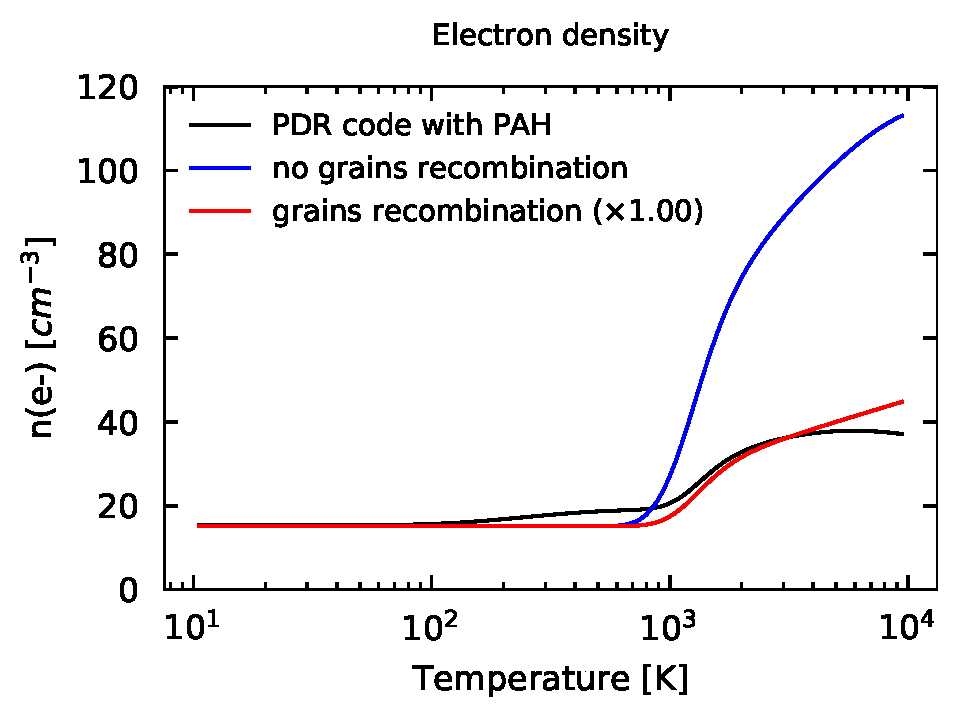
\includegraphics[trim = {0 0 0 1.5cm},clip,width=1\textwidth]{figure/Cl/model/test_calc_PAH_e.png}
        \caption{avec PAH}
    \end{subfigure}
    ~ 
    \begin{subfigure}[t]{0.45\textwidth}
        \centering 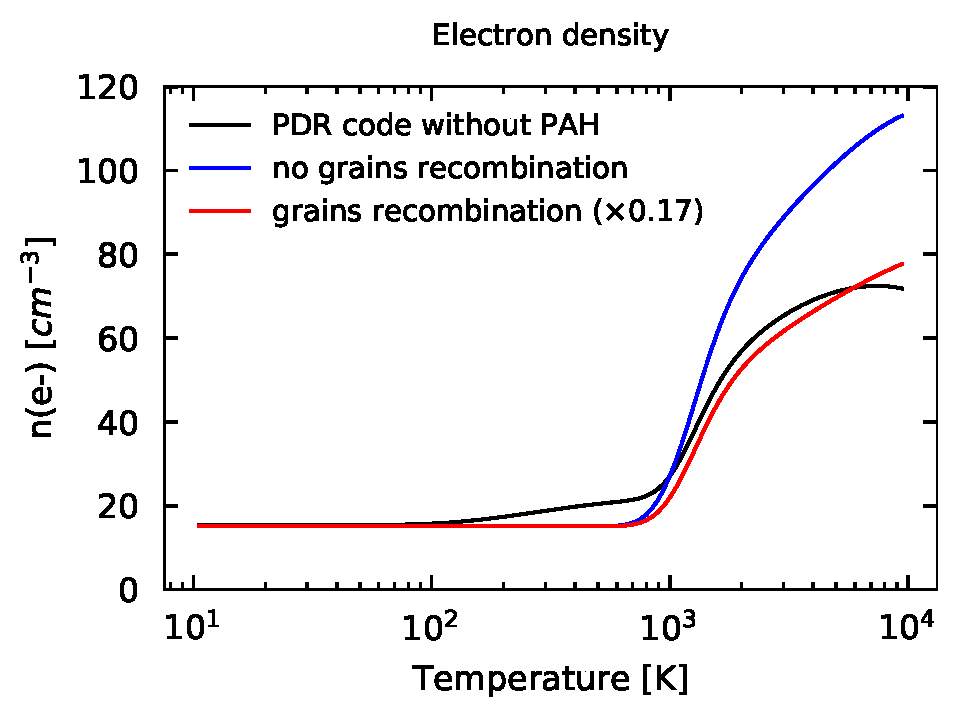
\includegraphics[trim = {0 0 0 1.5cm},clip,width=1\textwidth]{figure/Cl/model/test_calc_e.png}
        \caption{sans PAH}
    \end{subfigure}
    \caption{Profil de la densité électronique calculé par le modèle. La formule proposée par \cite{Weingartner_2001} prend en compte la recombinaison sur les PAH. Avec la recombinaison, la prédiction de la densité d'électrons est bonne dans le cas avec PAH. Si on ne prend pas en compte les PAH, il faut diminuer le taux de recombinaison d'un facteur $1/6$ pour prédire une densité d'électrons raisonnable.}
    \label{fig:Cl:model:rec}
\end{figure}



%%%%%%%%%%%%%%%%%%%%%%%%%%%%%%%%%%%%%%%%%%%%%%%%%%%%%%%%%%%%%%%%%%%%%%%%%%%%%%%%%%%%%%%%%%%%%%%
\subsection{Modèle analytique - Thermique}

On cherche la température d'équilibre du milieu dans différentes configurations de PDR. On considère dans ce modèle uniquement le chauffage par effet photoélectrique, le chauffage par $\mathrm{H}_2$ qui joue principalement dans les régions hautes densités et faible champs de rayonnement sera traité plus tard. On cherche $\Gamma = \Lambda $ en fonction de la température avec

\begin{equation}
    \begin{split}
        \Gamma &= \Gamma_{pe}^{\mathrm{Rollïg}} \\
        \Lambda &=   \Lambda_{\mathrm{CII}\ 158 \mu \mathrm{m}} + \Lambda_{\mathrm{OI}\ 63 \mu \mathrm{m}} + \Lambda_{\mathrm{OI}\ 146 \mu \mathrm{m}}  + \Lambda_{\mathrm{H}_\alpha} + \Lambda_{\mathrm{g}-\mathrm{g}} + \Lambda_{\mathrm{rec}}^{\mathrm{Rollïg}}
    \end{split}
\end{equation}


\subsubsection{Effet photoélectrique sur les grains}

De \cite{Rollig2005} (Eq (10) ou (C.3)) qui provient de \cite{BakesTielens1994}, sans PAH, on utilise : 

\begin{equation}
    \Gamma_{\mathrm{pe}} = 10^{-24}\,G_0\,n_\mathrm{H}\, \frac{2\times 10^{-2}}{1 + 2\times 10^{-4}\,G_0 \sqrt{T}/n_e} \operatorname{erg} \mathrm{cm}^{-3} \mathrm{s}^{-1}
\end{equation}

Avec $G_0 = 1.71\chi \times 0.5$ car il considère une illumination provenant que d'un coté. (\cite{Wolfire_2003} Eq 20, \cite{BakesTielens1994}) propose une autre formule prenant en compte les PAH qui est de la forme 

\begin{equation}
    \Gamma_{\mathrm{pe}}^{\mathrm{Wolf}} = 10^{-24}\,G_0\,n_\mathrm{H}\, \bbig[ \frac{4.9\times 10^{-2}}{1 + 4\times 10^{-3}\, \frac{G_0 \sqrt{T}}{n_e \phi_\mathrm{PAH}}} + \frac{3.7\times 10^{-2} (T/10^4)^{0.7}}{1 + 2\times 10^{-4}\, \frac{G_0 \sqrt{T}}{n_e \phi_\mathrm{PAH}}} \bbig] \operatorname{erg} \mathrm{cm}^{-3} \mathrm{s}^{-1}
\end{equation}

avec $\phi_\mathrm{PAH}$ une efficacité de collision compris entre 0 et 1. L'effet photoélectrique est d'autant plus efficace sur les petits grains \cite{DraineBook}. Le choix de $r_\mathrm{min}$ (la taille minimale des grains dans la description MRN) est décisif. Si l'on trace ces formules sur la \autoref{fig:Cl:pePAH} pour différent $\phi_\mathrm{PAH}$ et $r_\mathrm{min}$ on voit que la formule de \cite{Rollig2005} sous-estime le taux calculé par le code PDR de Meudon. Avec $r_\mathrm{min} = 1\,10^7\,\mathrm{nm}$, la prescription de Rollig est 3 fois plus petit que le chauffage calculé par Meudon. Si l'on augmente la taille de grain minimale, on voit que cette écart diminue ce qui est normale car l'on réduit l'efficacité de l'effet photo-électrique en enlevant les petits grains. La prescription de \cite{Wolfire_2003} laisse plus de liberté à travers le $\phi_\mathrm{PAH}$ (not much to say).

\begin{figure}[!h]
    \centering
    \begin{subfigure}[t]{0.45\textwidth} % "0.45" donne ici la largeur de l'image
        \centering 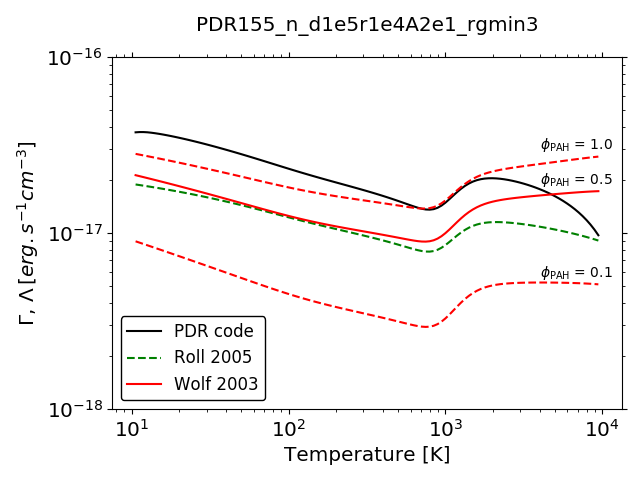
\includegraphics[trim = {0 0 0 1cm},clip,width=1\textwidth]{figure/Cl/pePAH/pe_formulae_rgmin3.png}
        \caption{$r_\mathrm{min} = 3\,10^{-7} \, \mathrm{nm}$}
    \end{subfigure}
    ~ 
   \begin{subfigure}[t]{0.45\textwidth} % "0.45" donne ici la largeur de l'image
        \centering 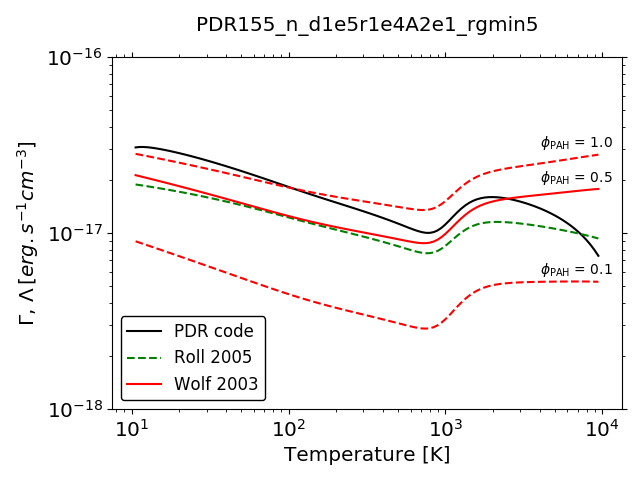
\includegraphics[trim = {0 0 0 1cm},clip,width=1\textwidth]{figure/Cl/pePAH/pe_formulae_rgmin5.png}
        \caption{$r_\mathrm{min} = 5\,10^{-7}\, \mathrm{nm}$}
    \end{subfigure}
    \caption{Comparaison des formules de l'effet photoélectrique de \cite{Rollig2005} et \cite{Wolfire_2003} avec le code PDR utilisant différents $r_\mathrm{min}$}
    \label{fig:Cl:pePAH}
\end{figure}

%%%%%%%%%%%%%%%%%%%%%%%%%%%%%%%%%%%%%%%%%%%%%%%%%%%%%%%%%%%%%%%%%%%%%%%%%%%%%%%%%%%%%%%%%%%%%%%

\subsubsection{Couplage gaz-grains}

De \cite{Rollig2005} ($Z=1$), le couplage gaz grain s'exprime,

\begin{equation}
    \Lambda_{\mathrm{g}-\mathrm{g}} = 3.5\,10^{-34}\times \sqrt{T}(T - T_g) {n_\mathrm{H}}^2 \operatorname{erg} \mathrm{cm}^{-3} \mathrm{s}^{-1}
\end{equation}

Où $T_g$ est donné par Eq. 6 de \cite{HollenbachTakahashiTielens_1991}
\begin{equation}
    T_g = 12.2 \,{G_0}^{0.2}
\end{equation}

%%%%%%%%%%%%%%%%%%%%%%%%%%%%%%%%%%%%%%%%%%%%%%%%%%%%%%%%%%%%%%%%%%%%%%%%%%%%%%%%%%%%%%%%%%%%%%%


\subsubsection{Refroidissement par les raies d'émissions du $\mathrm{C}^+$ et de $\mathrm{O}$}

[CII]$158 \mu \mathrm{m}$, provient de \cite{Rollig2005}, Equation (A.2) ($Z=1$)

\begin{equation}
    \Lambda_{\mathrm{CII}\ 158   \mu \mathrm{m}}= n(\mathrm{C}^+) \frac{2.89 \times 10^{-20}}{1+\frac{1}{2} \exp (92 / T)\left(1+\frac{1300}{n_\mathrm{H}}\right)} \operatorname{erg} \mathrm{cm}^{-3} \mathrm{s}^{-1}
\end{equation}

Pour les raies de [OI], Rollïg prend en compte les transitions adjacentes de [OI]$62 \mu \mathrm{m}$ et $[OI]146 \mu \mathrm{m}$. ($Z$,$\beta = 1$)


\begin{equation}
\begin{split}
    \Lambda_{\mathrm{OI}\ 63 \mu \mathrm{m}} &= 3.15\,10^{-14} \times 8.46\,10^{-5} \times 
    n(\mathrm{O}) \\
    & \times \frac{e^{98/T} 3 n_\mathrm{H} (n_\mathrm{H} + \beta\, n_{\mathrm{cr}_{01}} ) }{{n_\mathrm{H}}^2+ e^{98/T}(n_\mathrm{H} + \frac{1}{2} n_{\mathrm{cr}_{01}} ) (3 n_\mathrm{H} + 5\, e^{228/T} (n_\mathrm{H} + \frac{1}{2} n_{\mathrm{cr}_{12}} )) } \operatorname{erg} \mathrm{cm}^{-3} \mathrm{s}^{-1}
\end{split}
\end{equation}

\begin{equation}
\begin{split}
    \Lambda_{\mathrm{OI}\ 146 \mu \mathrm{m}} &= 1.35\,10^{-14} \times 8.46\,10^{-5} \times 
    n(\mathrm{O}) \\
    & \times \frac{ {n_\mathrm{H}}^2 }{n_\mathrm{H}^2+ e^{98/T}(n_\mathrm{H} + \frac{1}{2} n_{\mathrm{cr}_{01}} ) (3 n_\mathrm{H} + 5\, e^{228/T} (n_\mathrm{H} + \frac{1}{2} n_{\mathrm{cr}_{12}} )) } \operatorname{erg} \mathrm{cm}^{-3} \mathrm{s}^{-1}
\end{split}
\end{equation}

Avec $n_{\mathrm{cr}_{01}}(T) = \frac{1.66\,10^{-5} }{1.35\,10^{-11} T^{0.45}} $ et $n_{\mathrm{cr}_{12}}(T) = \frac{8.46\,10^{-5} }{4.37\,10^{-12} T^{0.66}} $

%%%%%%%%%%%%%%%%%%%%%%%%%%%%%%%%%%%%%%%%%%%%%%%%%%%%%%%%%%%%%%%%%%%%%%%%%%%%%%%%%%%%%%%%%%%%%%%

\subsubsection{Emission Lyman $\mathrm{H}\alpha$}

\cite{tielens2005}, Eq 2.62

\begin{equation}
    \Lambda_{\mathrm{H}\alpha} = 7.3\, 10^{-19}\,n_e\,n_\mathrm{H}\,e^{-118400/T} \operatorname{erg} \mathrm{cm}^{-3} \mathrm{s}^{-1}
\end{equation}

%%%%%%%%%%%%%%%%%%%%%%%%%%%%%%%%%%%%%%%%%%%%%%%%%%%%%%%%%%%%%%%%%%%%%%%%%%%%%%%%%%%%%%%%%%%%%%%

\subsubsection{Recombinaison des électrons sur les grains}

Dans le modèle de chlore, on prend celle de \cite{Rollig2005} Eq.4  qui provient elle même de \cite{BakesTielens1994}.

\begin{equation}
    \Lambda_{\mathrm{rec}}^{\mathrm{Rollïg}} = 3.49\,10^{-30} T^{0.944} \, (\frac{G_0 \sqrt{T}}{n_e})^{\frac{0.735}{T^{0.068}}} \, n_e \, n_\mathrm{H} \operatorname{erg} \mathrm{cm}^{-3} \mathrm{s}^{-1}
\end{equation}

Il existe également celle ci \cite{WolfireHollenbachMcKeeTielensBakes_1995} Eq. 9 que l'on n'utilise pas.

\begin{equation}
    \Lambda_{\mathrm{rec}}^{\mathrm{Wolfire}} = 4.65\,10^{-30} T^{0.94} \, (\frac{G_0 \sqrt{T}}{n_e})^{\frac{0.74}{T^{0.068}}} \, n_e \, n_\mathrm{H} \operatorname{erg} \mathrm{cm}^{-3} \mathrm{s}^{-1}
\end{equation}

%%%%%%%%%%%%%%%%%%%%%%%%%%%%%%%%%%%%%%%%%%%%%%%%%%%%%%%%%%%%%%%%%%%%%%%%%%%%%%%%%%%%%%%%%%%%%%%

\subsection{Prédiction de la température au bord de nuage}
\subsubsection{Carte de température en bord atomique du nuage}

Que fait le modèle ? On trace en fonction de la température le terme de chauffage $\Gamma$ et $\Lambda$ à partir de la densité d'électrons $n_e$ que l'on obtient à partir du modèle chimique. On cherche les $T_{eq}$ tel que $\Gamma - \Lambda  = 0$ que l'on caractérise de stable si autour du point d'équilibre $\frac{d}{dT}(\Gamma - \Lambda) <0$ et d'instable sinon. On visualise sur \autoref{fig:Cl:grid:mapT} la température maximale atteignable par le bord atomique. La zone hachurée indique les solutions instables.

\textit{Conséquences dynamiques : Hydra d'Emeric}

\begin{figure}[htbp]
    \centering
    \begin{subfigure}[t]{0.45\textwidth} % "0.45" donne ici la largeur de l'image
        \centering \includegraphics[trim = {0 0 0 1.5cm},clip,width=1\textwidth]{figure/Cl/model/mapG0nHTeq_pe_OI_CII_ggr_elecrec_lyman_OI_imp.png}
        \caption{avec chlore}
    \end{subfigure}
    ~ 
    \begin{subfigure}[t]{0.45\textwidth}
        \centering \includegraphics[trim = {0 0 0 1.5cm},clip,width=1\textwidth]{figure/Cl/model/mapG0nHTeq_pe_OI_CII_ggr_elecrec_lyman_OI_noCl.png}
        \caption{sans chlore}
    \end{subfigure}
    \caption{Carte de la température en bord de nuage atomique ($A_\mathrm{V}= 10^{-6}$) prédit par le modèle.}
    \label{fig:Cl:model:mapT}
\end{figure}

Si l'on prend en compte la recombinaison sur les grains, la prédiction des la densité d'électrons devient quantitavement proche de celle que calculerait le modèle. En retracant les cartes de températures (\autoref{}) on se rend compte qu'elles ne sont pas beaucoup modifiées.

\subsubsection{Grille de modèles}

Les grilles de modèle de la version du code \uncinq donne des cartes de température plotée sur la \autoref{fig:Cl:grid:mapT}. Le même quadrant est impacté bien que la solution haute ne soit pas toujours atteinte. La région faible champs de rayonnement et haute densité est prédominée par le chauffage par la molécule $\mathrm{H}_2$ qui n'est pas pris en compte dans ce petit modèle.  

\textit{Que se passe t'il à faible densité ? Pourquoi n'a t on pas les tangentes horizontales de T ?}

\begin{figure}[!htbp]
    \centering
    \begin{subfigure}[t]{0.45\textwidth} % "0.45" donne ici la largeur de l'image
        \centering 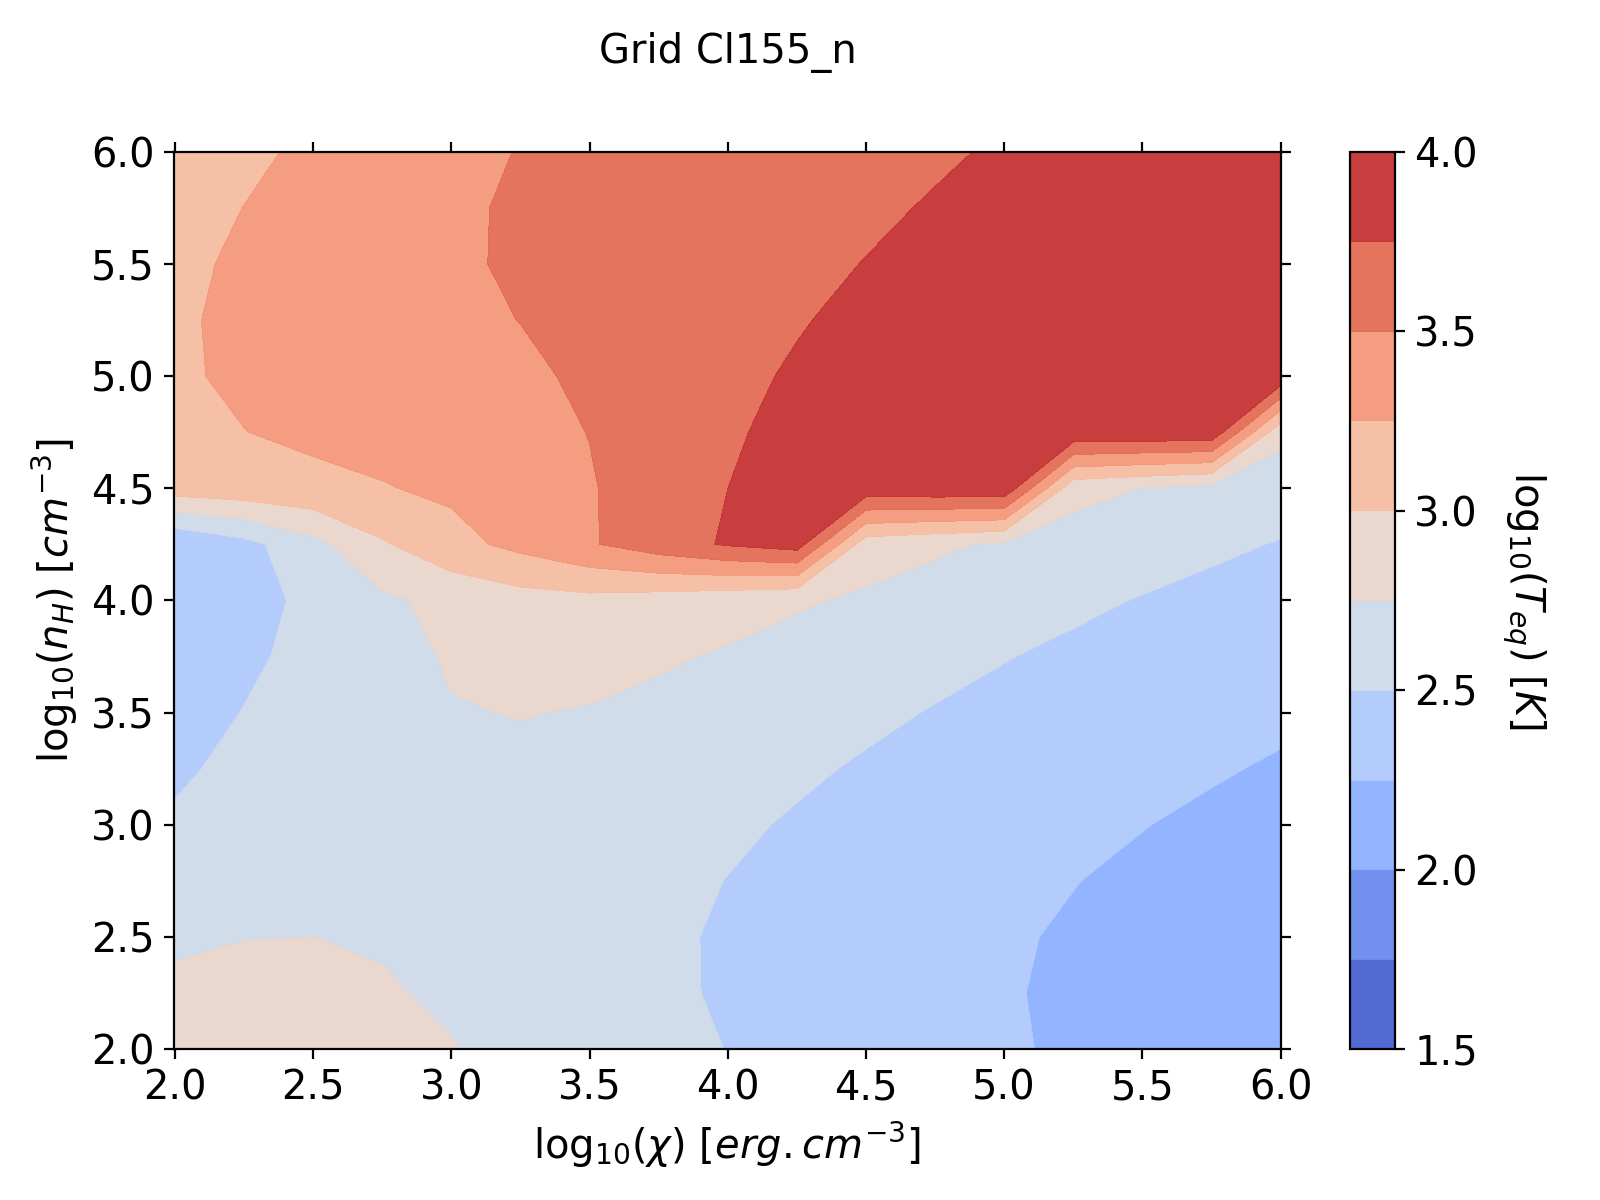
\includegraphics[trim = {0 0 0 1.5cm},clip,width=1\textwidth]{figure/Cl/grid/mapTCl.png}
        \caption{avec chlore}
    \end{subfigure}
    ~ 
    \begin{subfigure}[t]{0.45\textwidth}
        \centering 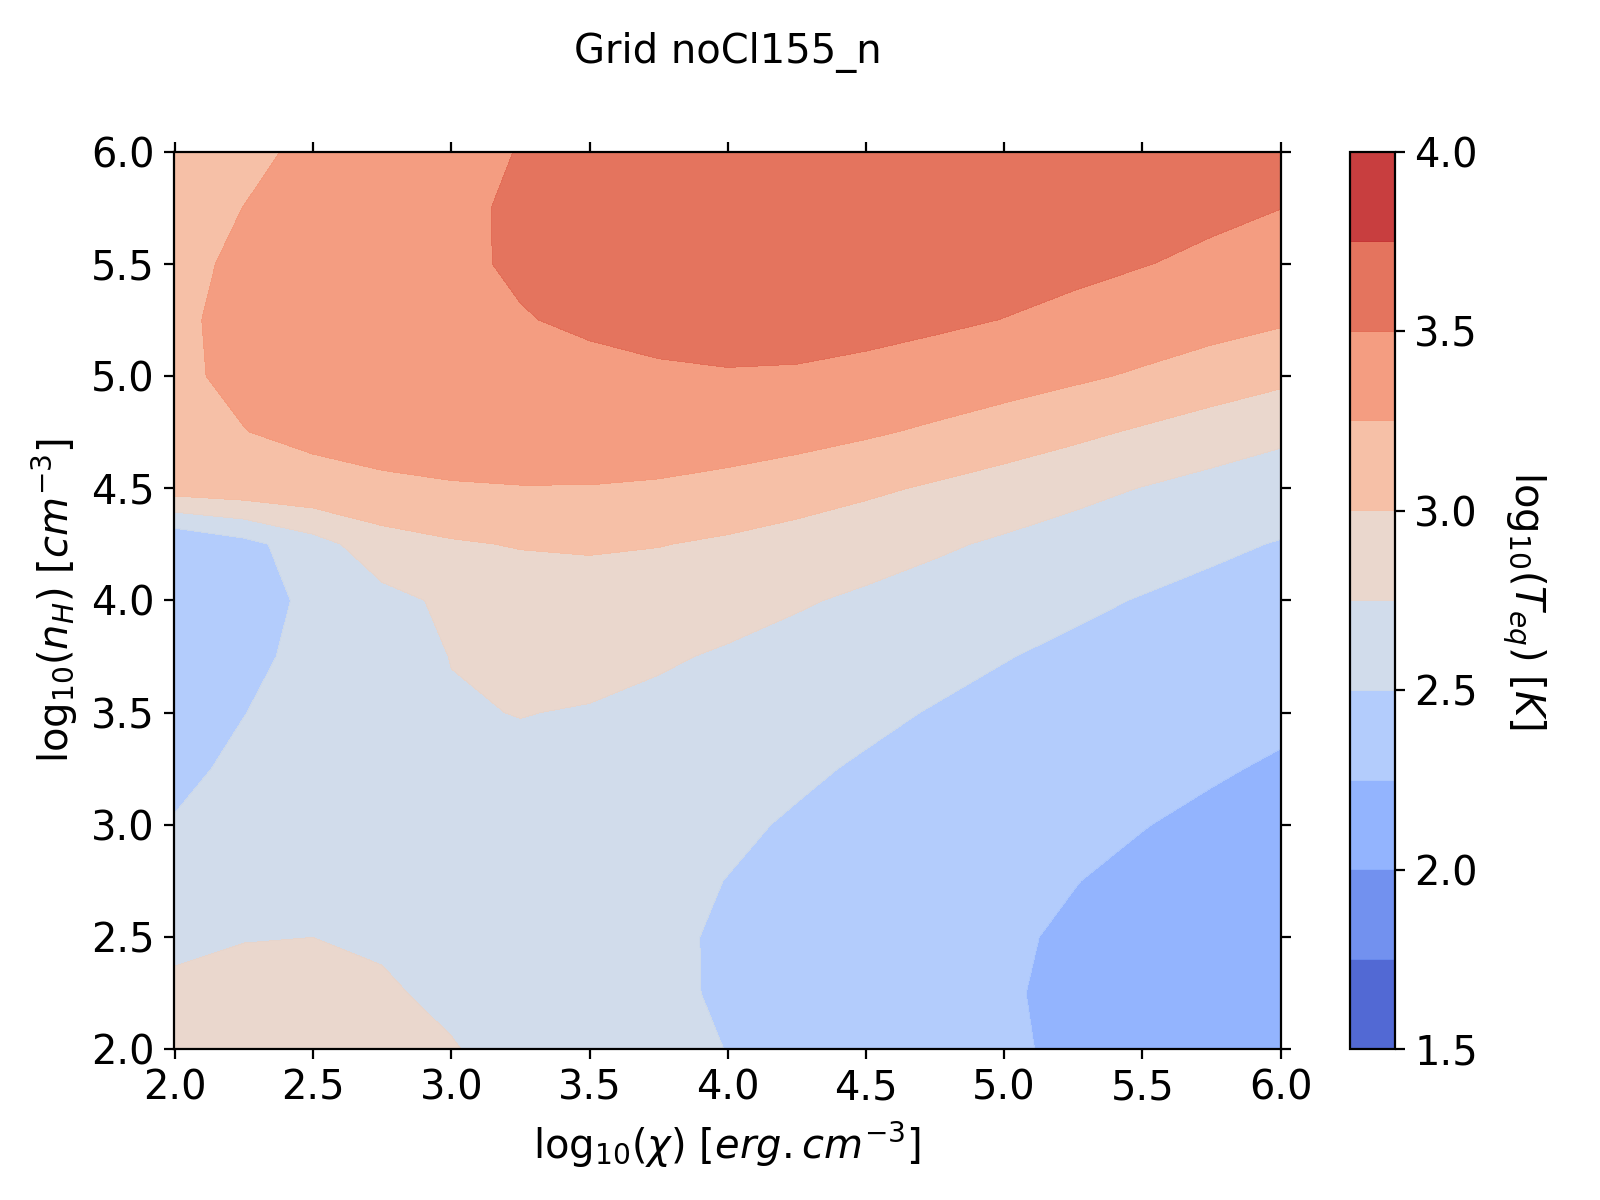
\includegraphics[trim = {0 0 0 1.5cm},clip,width=1\textwidth]{figure/Cl/grid/mapT.png}
        \caption{sans chlore}
    \end{subfigure}
    \caption{Température en bord de nuage atomique ($A_\mathrm{V}= 10^{-6}$) calculé par le code PDR \uncinq. Les PAH et la recombinaison du $\mathrm{H}^+ $ sur les grains n'ont pas été pris en compte.}
    \label{fig:Cl:grid:mapT}
\end{figure}

On a discuté précédemment de la prescription de Rollig qui sous-estime l'efficacité de l'effet photoélectrique pour des modèles de PDR avec une taille minimale de grains de $1\,10^{-7} \, \mathrm{nm}$. Si l'on corrige d'un facteur 3 le taux de chauffage c.a.d. que l'on prend un $\Gamma_{pe}^{'} = 3 \times \Gamma_{pe}^{Rollïg}$, on obtient une nouvelle carte de température assez différente.


\subsubsection{Chauffage à l'entrée du nuage moléculaire}

Il arrive qu'en entrée du nuage moléculaire, la température du gaz augmente de manière irrégulière. Dans cette région, l'effet photoélectrique devient encore plus efficace en raison de l'augmentation de la fraction électronique du nuage. La recombinaison sur les grains est rapide s'il y a une quantité importante d'électron autour des grains. Dans cette zone, le $\mathrm{H}_2$ tente de se former. La voie principale de formation passe par l'association radiative :

\begin{equation}
    \begin{array}{lccccclr}
       \mathrm{H}  & + & e^- & \rightarrow & \mathrm{H}^{-} & + & h\nu &  \\
    \end{array}
\end{equation}

suivi d'un détachement associatif :

\begin{equation}
    \begin{array}{lcccccclr}
       \mathrm{H}  & + &  \mathrm{H}^- & \rightarrow & \mathrm{H}_2 & + & e^- & + & KE\\
    \end{array}
\end{equation}

Cette réaction peut produire des électrons en quantité si elle devient dominante ce qui est le cas autour de $A_\mathrm{v} \approx 0.5 \mathrm{mag}$ sur \autoref{fig:Cl:grid:proH}. La formation du $\mathrm{H}_2$ déclenche également une chimie chaude permettant notamment de former le doux $\mathrm{CH}^+$ que l'on observe. Cette augmentation de température ne doit pas être confondue avec l'emballement provoqué par le Chlore.


\begin{figure}[!htbp]
    \centering
        \centering 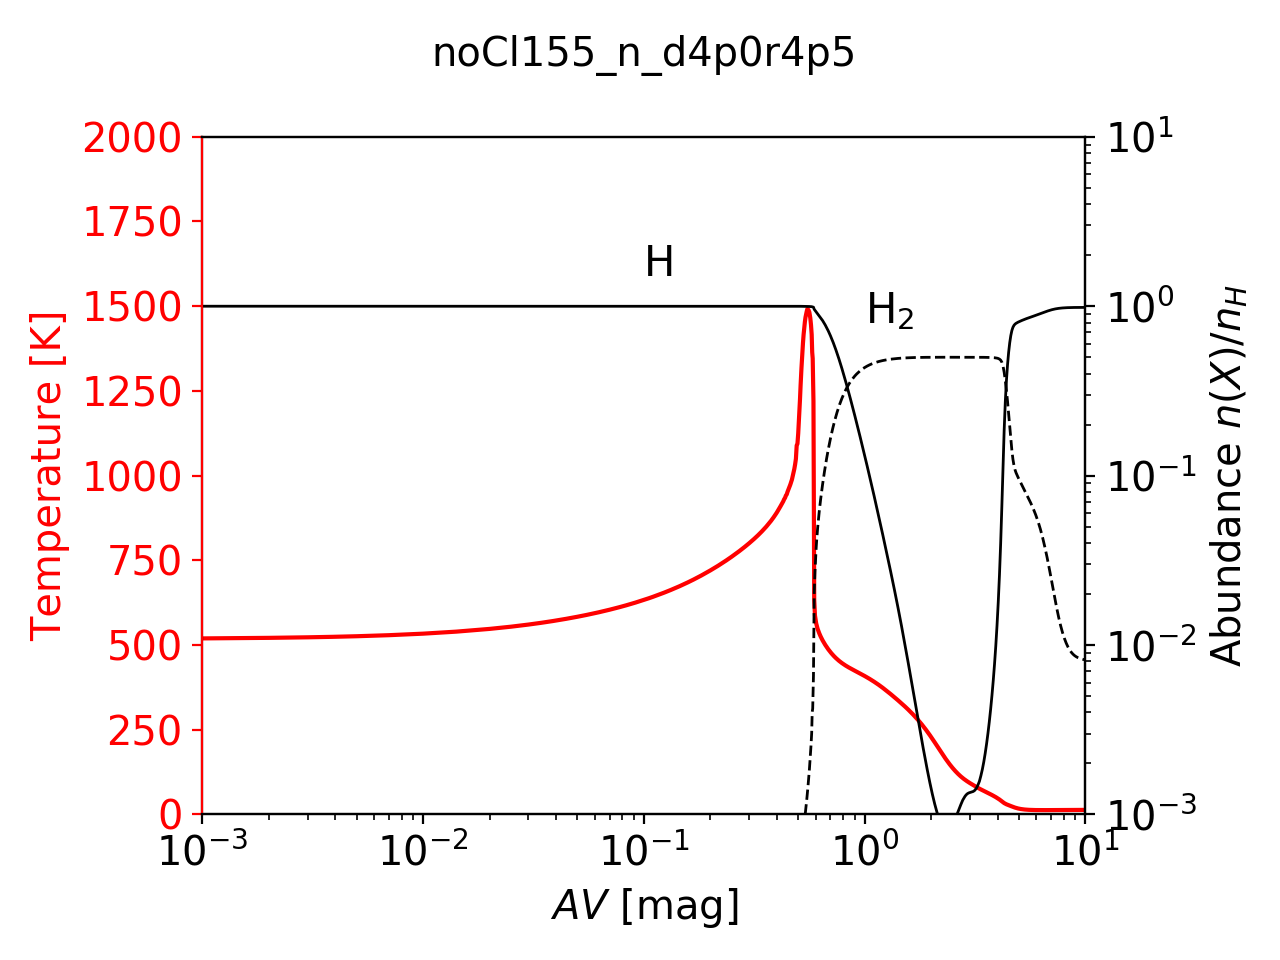
\includegraphics[trim = {0 0 0 1.5cm},clip,width=0.6\textwidth]{figure/Cl/grid/profil_H.png}
        \caption{...}
    \label{fig:Cl:grid:proH}
\end{figure}

\subsection{Diagramme d'état}

\subsection{Traceurs modifiés par le chlore}

On a pu extraire à partir des grilles calculé par le code (\uncinq) les raies d'émissions de chaques modèles et tracer des cartes d'intensités dans l'espace des paramètres et visualiser les spectres des traceurs impactés par l'ajout du chlore dans la chimie. On a étudié de 5 calculs de PDR, avec ou sans chlore, ayant des conditions physiques différentes afin de comparer localement le modèle au code de Meudon. Les 5 cas correspondent aux noms des modèles : 1. d5p0r4p5, 2. d4p0r4p5, 3. d3p0r4p5, 4. d3p0r3p0,  5. d5p0r3p0. \textbf{Cl155\_n} et \textbf{noCl155\_n} correspondent à des modèles à densité constante avec ou sans chlore de la version \uncinq.

\begin{figure}[!htbp]
    \centering
        \centering 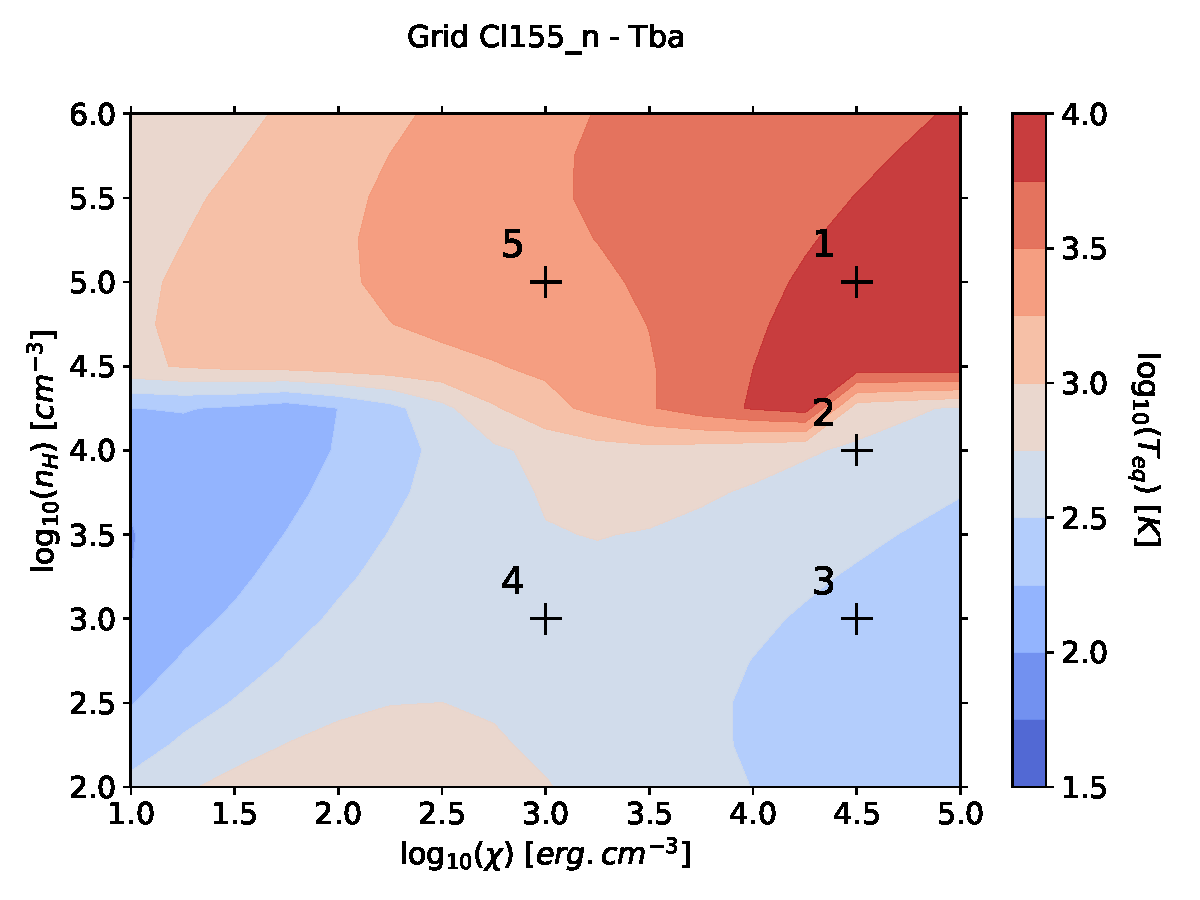
\includegraphics[trim = {0 0 0 1.5cm},clip,width=0.6\textwidth]{figure/Cl/grid/mapT_cross.pdf}
        \caption{Modèles utilisées pour les traceurs. Les modèles 1 et 2 sont directement concernés par l'ajout du chlore dans le code PDR. Seulement, le code parvient à trouver la solution haute que pour le calcul haute densité (1). Les cas 3, 4 et 5 explore les recoins de l'espace des paramètres. }
\end{figure}

\subsubsection{Diagramme d'excitation}

L'ajout du chlore augmente certaines du $\mathrm{N}$, $\mathrm{N}^+$, $\mathrm{S}$, $\mathrm{Si}$ comme on le voit sur la figure (\autoref{fig:Cl:gridModelEmiss:yes}). La solution chaude avec chlore peut avoir des raies d'un facteur 10 fois plus importante. Le changement le plus remarquable est l'azote atomique. Les traceurs pas impactés sont $\mathrm{CS}$, $\mathrm{H}_2\mathrm{O}$, $\mathrm{H}_2$ et le $\mathrm{CO}$. L'ajout du chlore diminue même l'intensité de certaines raies tels que celles du $\mathrm{CS}$ ou $\mathrm{H}_2\mathrm{O}$ Enfin (annexe) les diagrammes d'excitations pour les modèles 3-4-5 ne sont nullement impactés par l'ajout du chlore : ce qui voudrait dire que l'impact du chlore serait confiné dans la région que l'on a determiné.

\begin{figure}[!htbp]
    \centering
    \begin{subfigure}[t]{0.45\textwidth} % "0.45" donne ici la largeur de l'image
        \centering 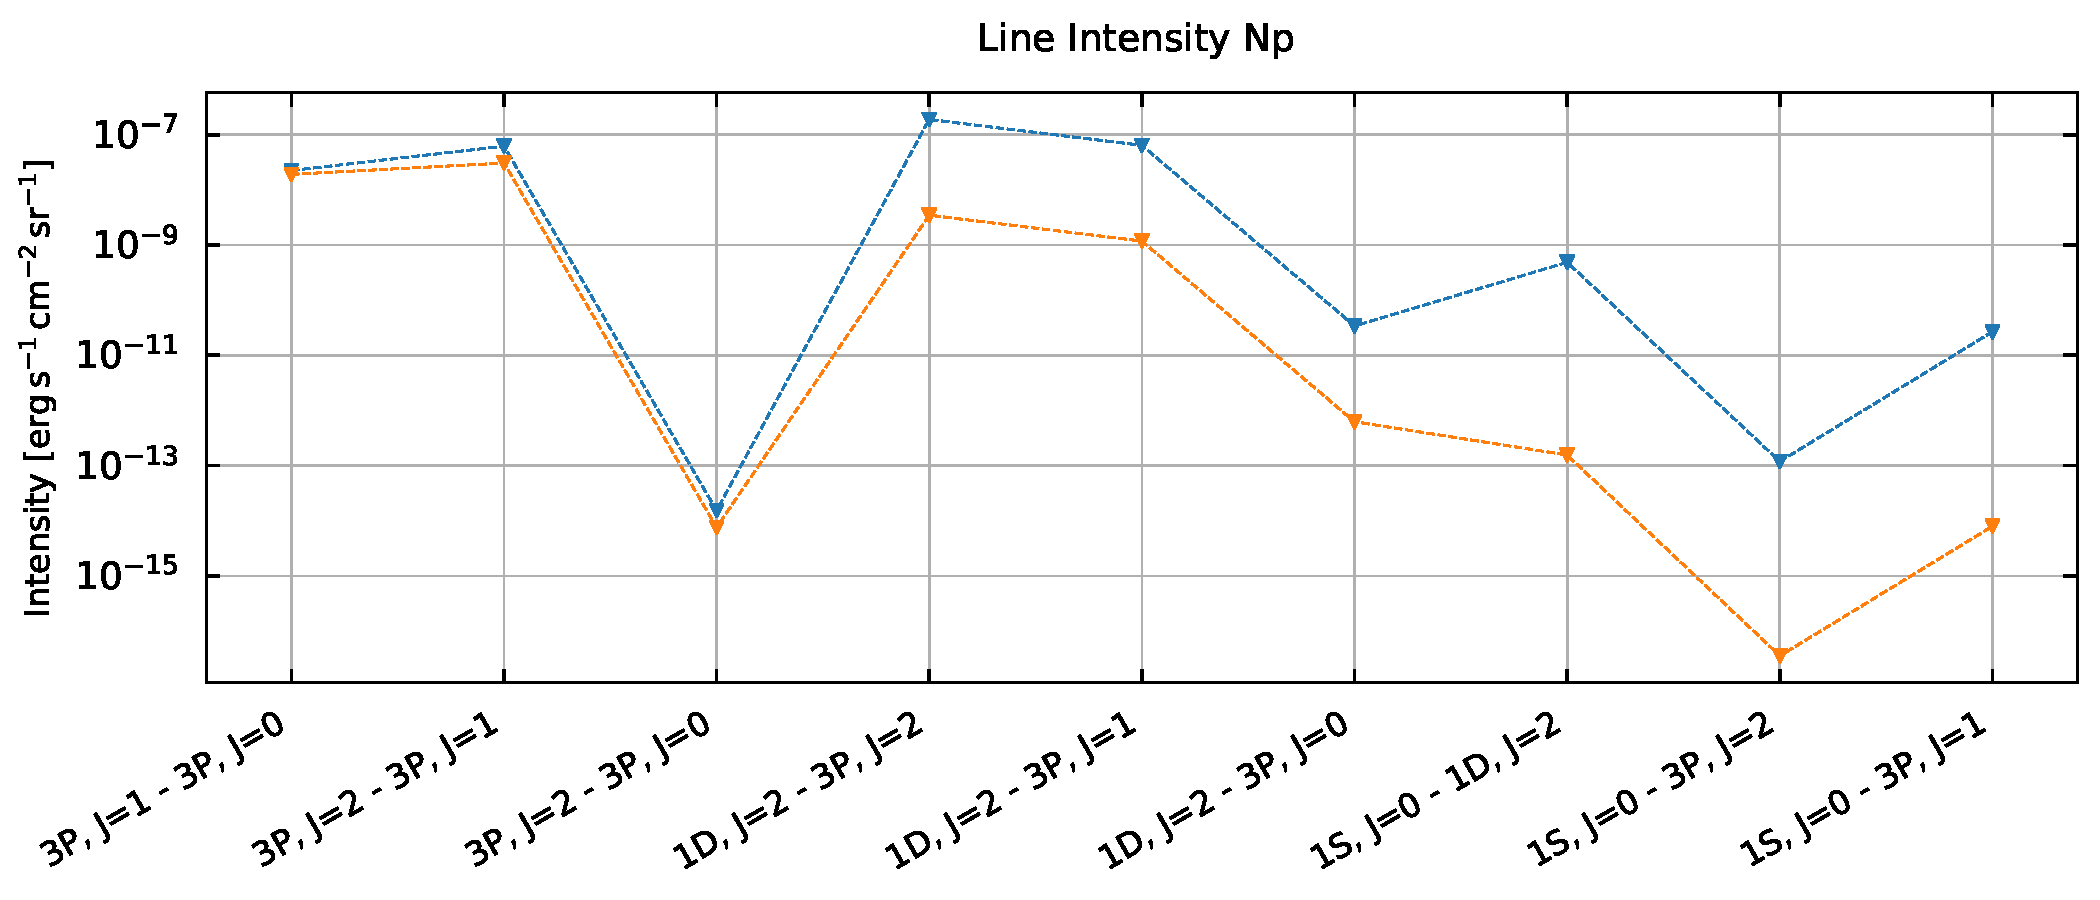
\includegraphics[trim = {0 0 0 1.5cm},clip,width=1\textwidth]{figure/Cl/gridModelEmiss/I_comp_Np.pdf}
        \caption{$\mathrm{N}^+$}
    \end{subfigure}
    ~ 
   \begin{subfigure}[t]{0.45\textwidth} % "0.45" donne ici la largeur de l'image
        \centering 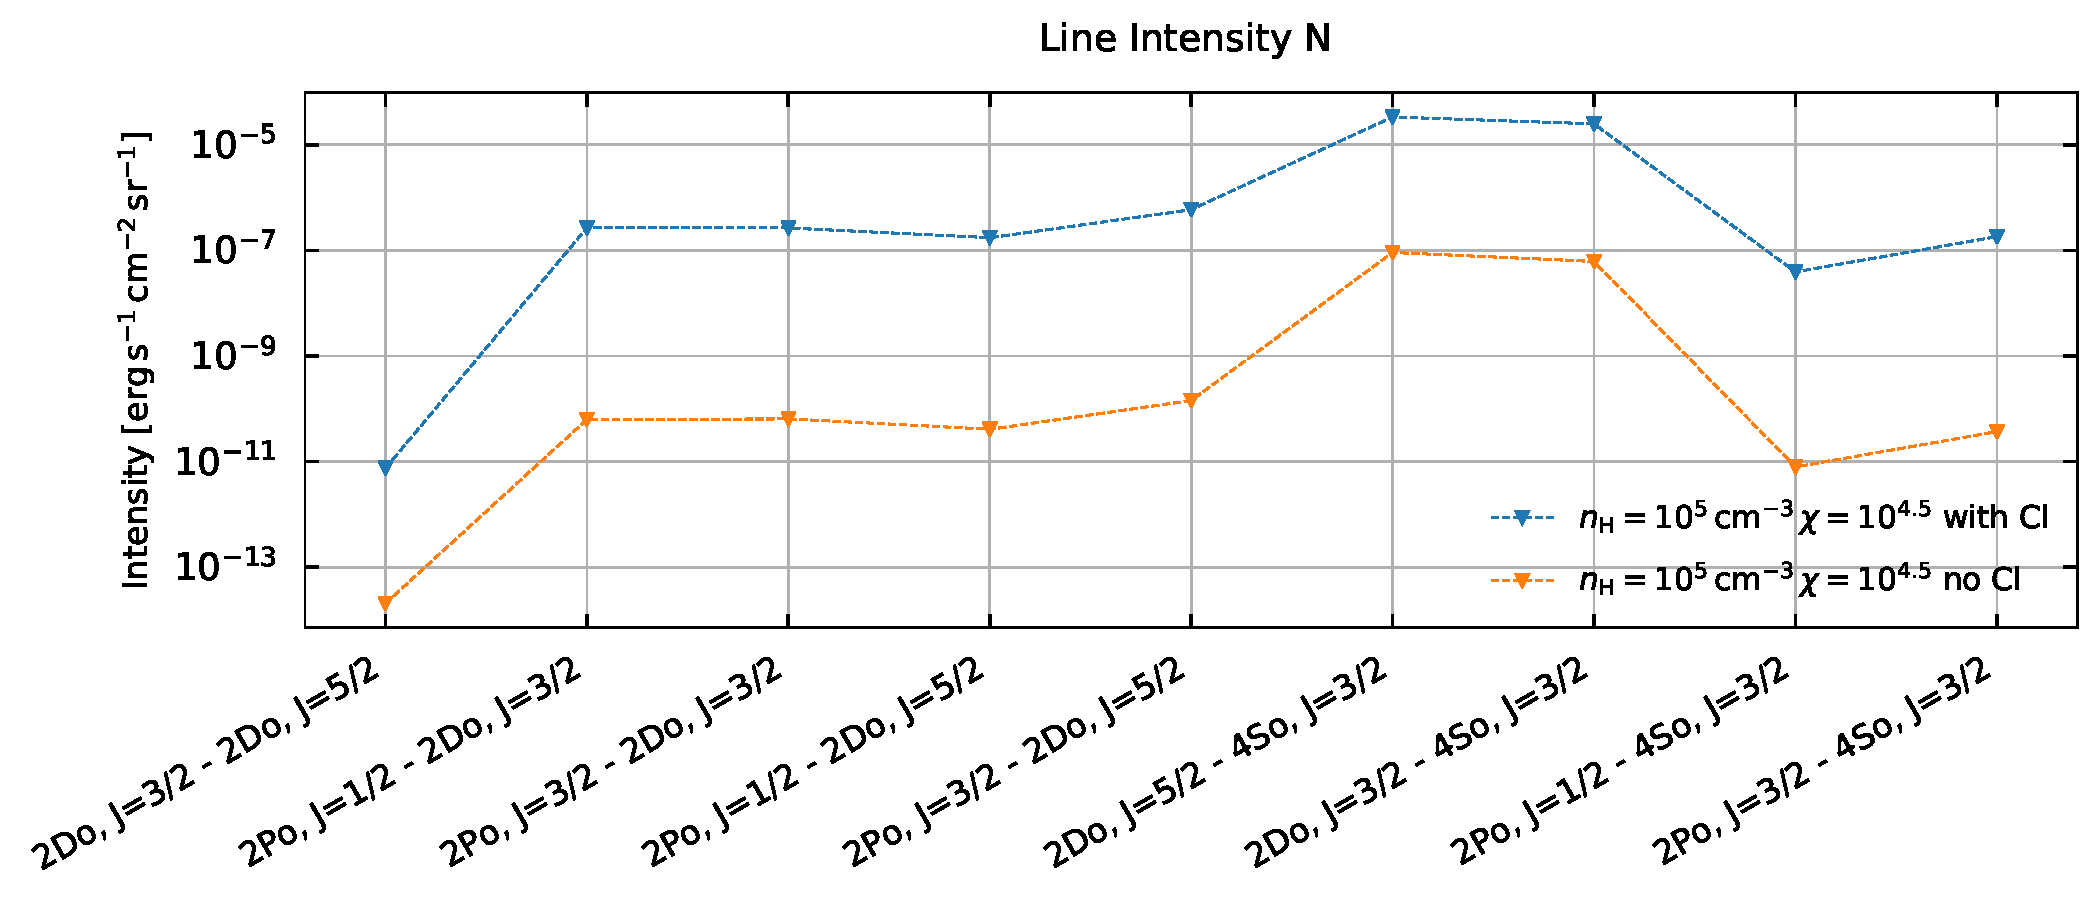
\includegraphics[trim = {0 0 0 1.5cm},clip,width=1\textwidth]{figure/Cl/gridModelEmiss/I_comp_N.pdf}
        \caption{$\mathrm{N}$}
    \end{subfigure}
    
    \begin{subfigure}[t]{0.45\textwidth} % "0.45" donne ici la largeur de l'image
        \centering 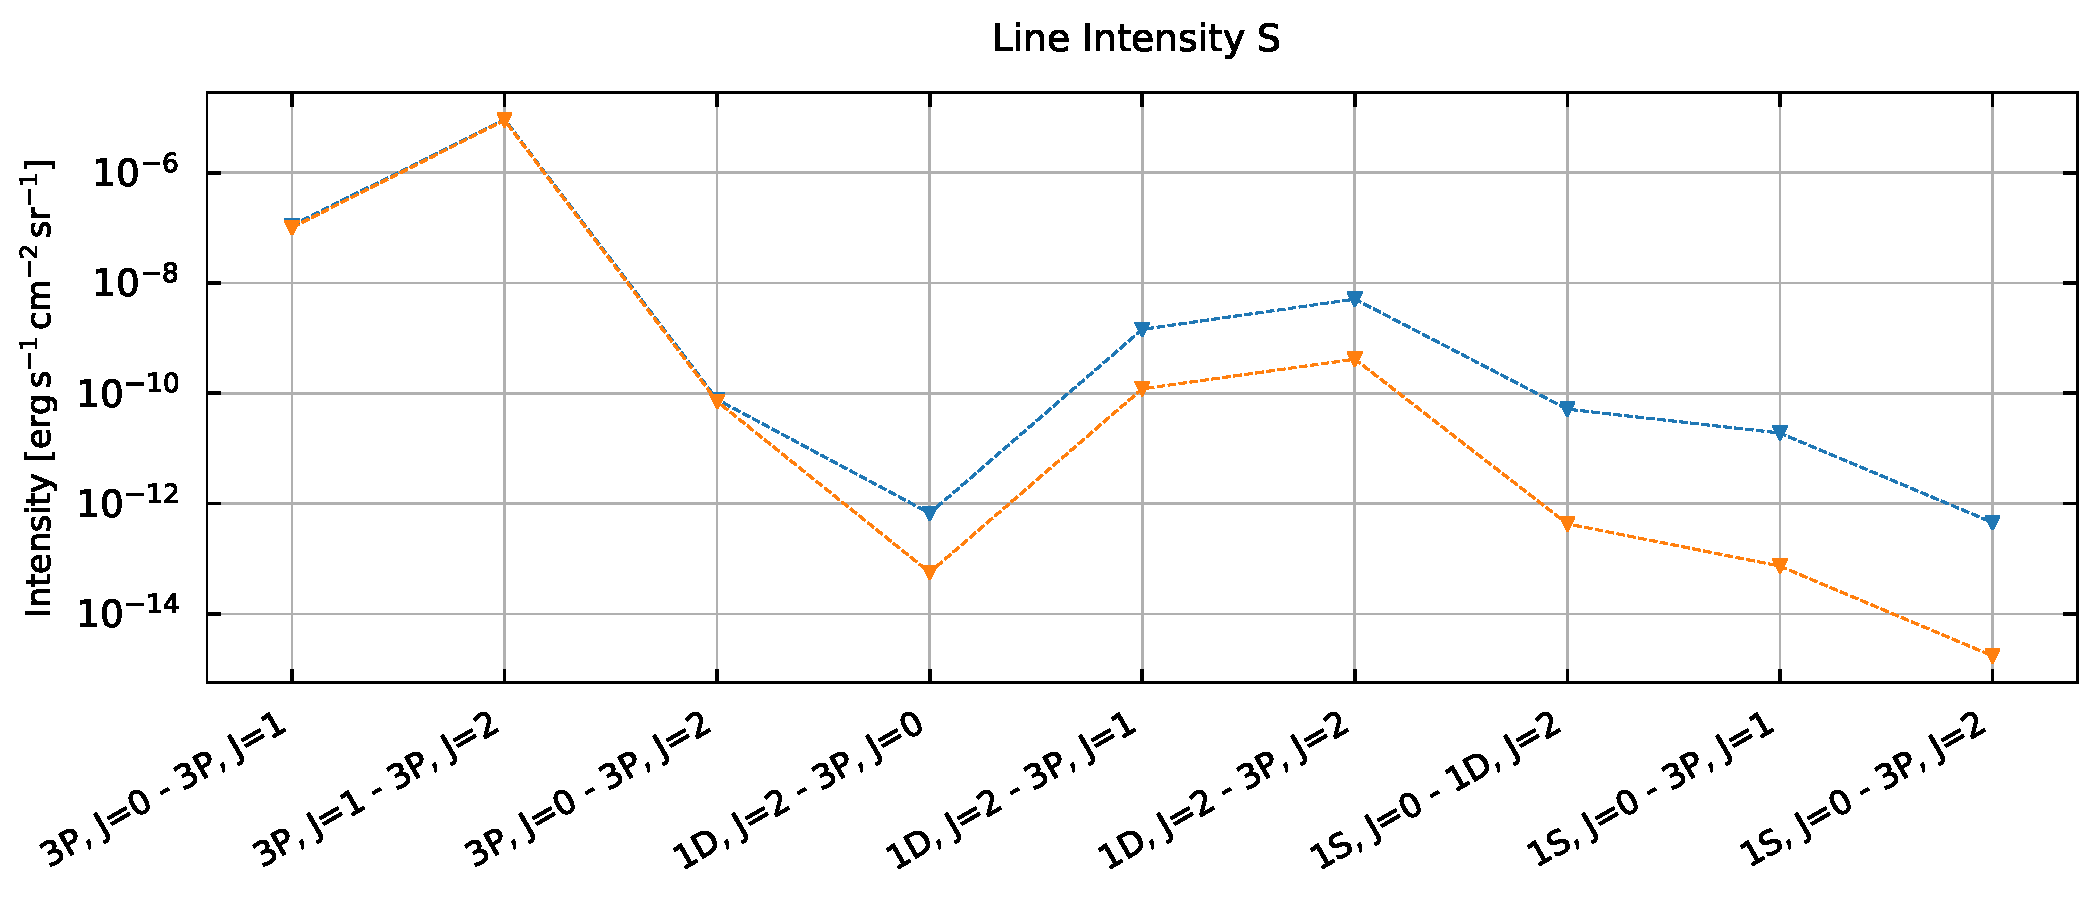
\includegraphics[trim = {0 0 0 1.5cm},clip,width=1\textwidth]{figure/Cl/gridModelEmiss/I_comp_S.pdf}
        \caption{$\mathrm{S}$}
    \end{subfigure}
    ~
    \begin{subfigure}[t]{0.45\textwidth} % "0.45" donne ici la largeur de l'image
        \centering 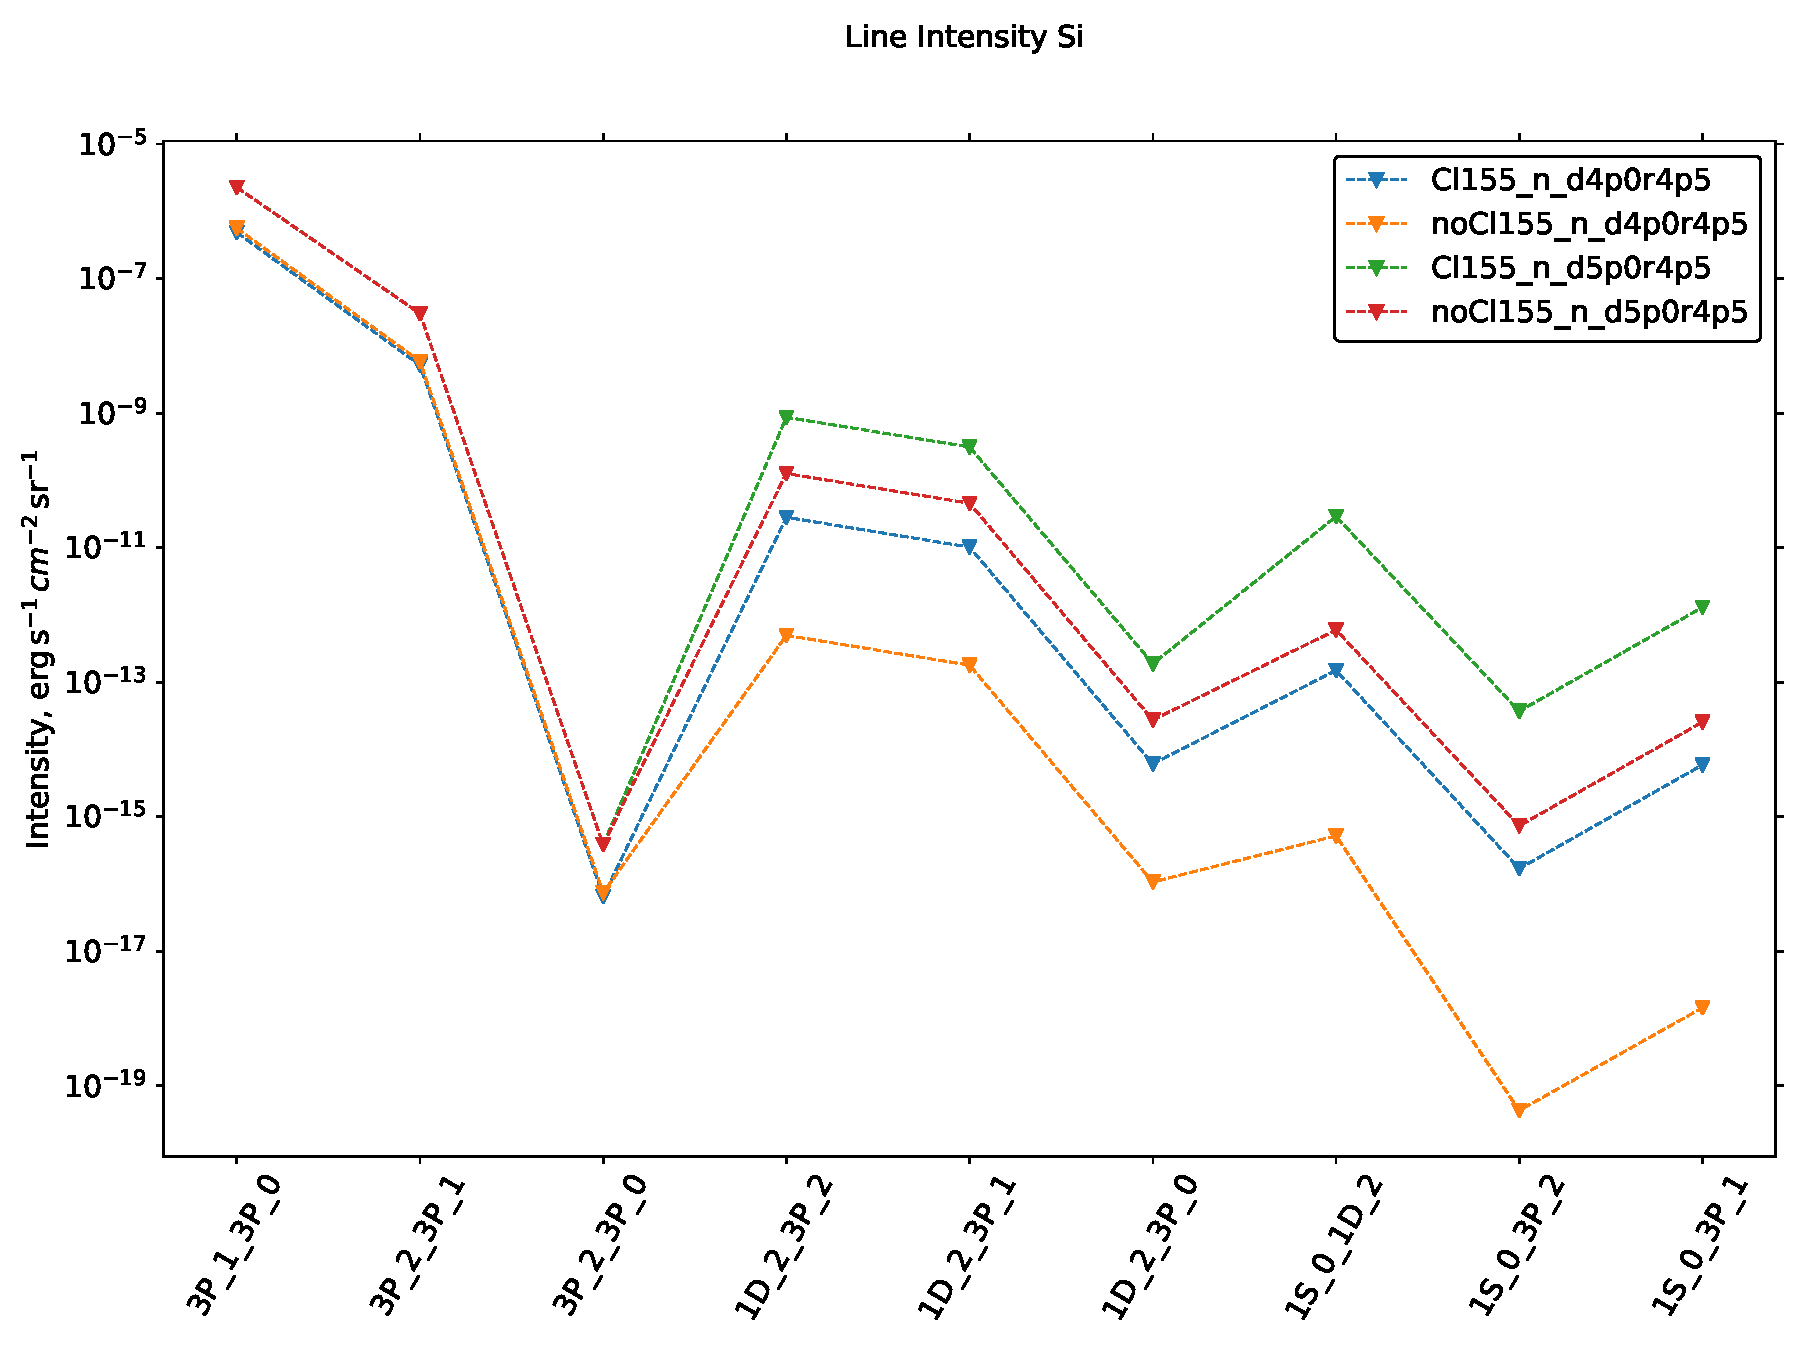
\includegraphics[trim = {0 0 0 1.5cm},clip,width=1\textwidth]{figure/Cl/gridModelEmiss/I_comp_Si.pdf}
        \caption{$\mathrm{Si}$}
    \end{subfigure}
    
    \caption{Diagramme d'excitation des traceurs modifiés par l'ajout du chlore dans le code PDR (\uncinq)}
    \label{fig:Cl:gridModelEmiss:yes}
\end{figure}

\begin{figure}[!htbp]
    \centering
    \begin{subfigure}[t]{0.45\textwidth} % "0.45" donne ici la largeur de l'image
        \centering 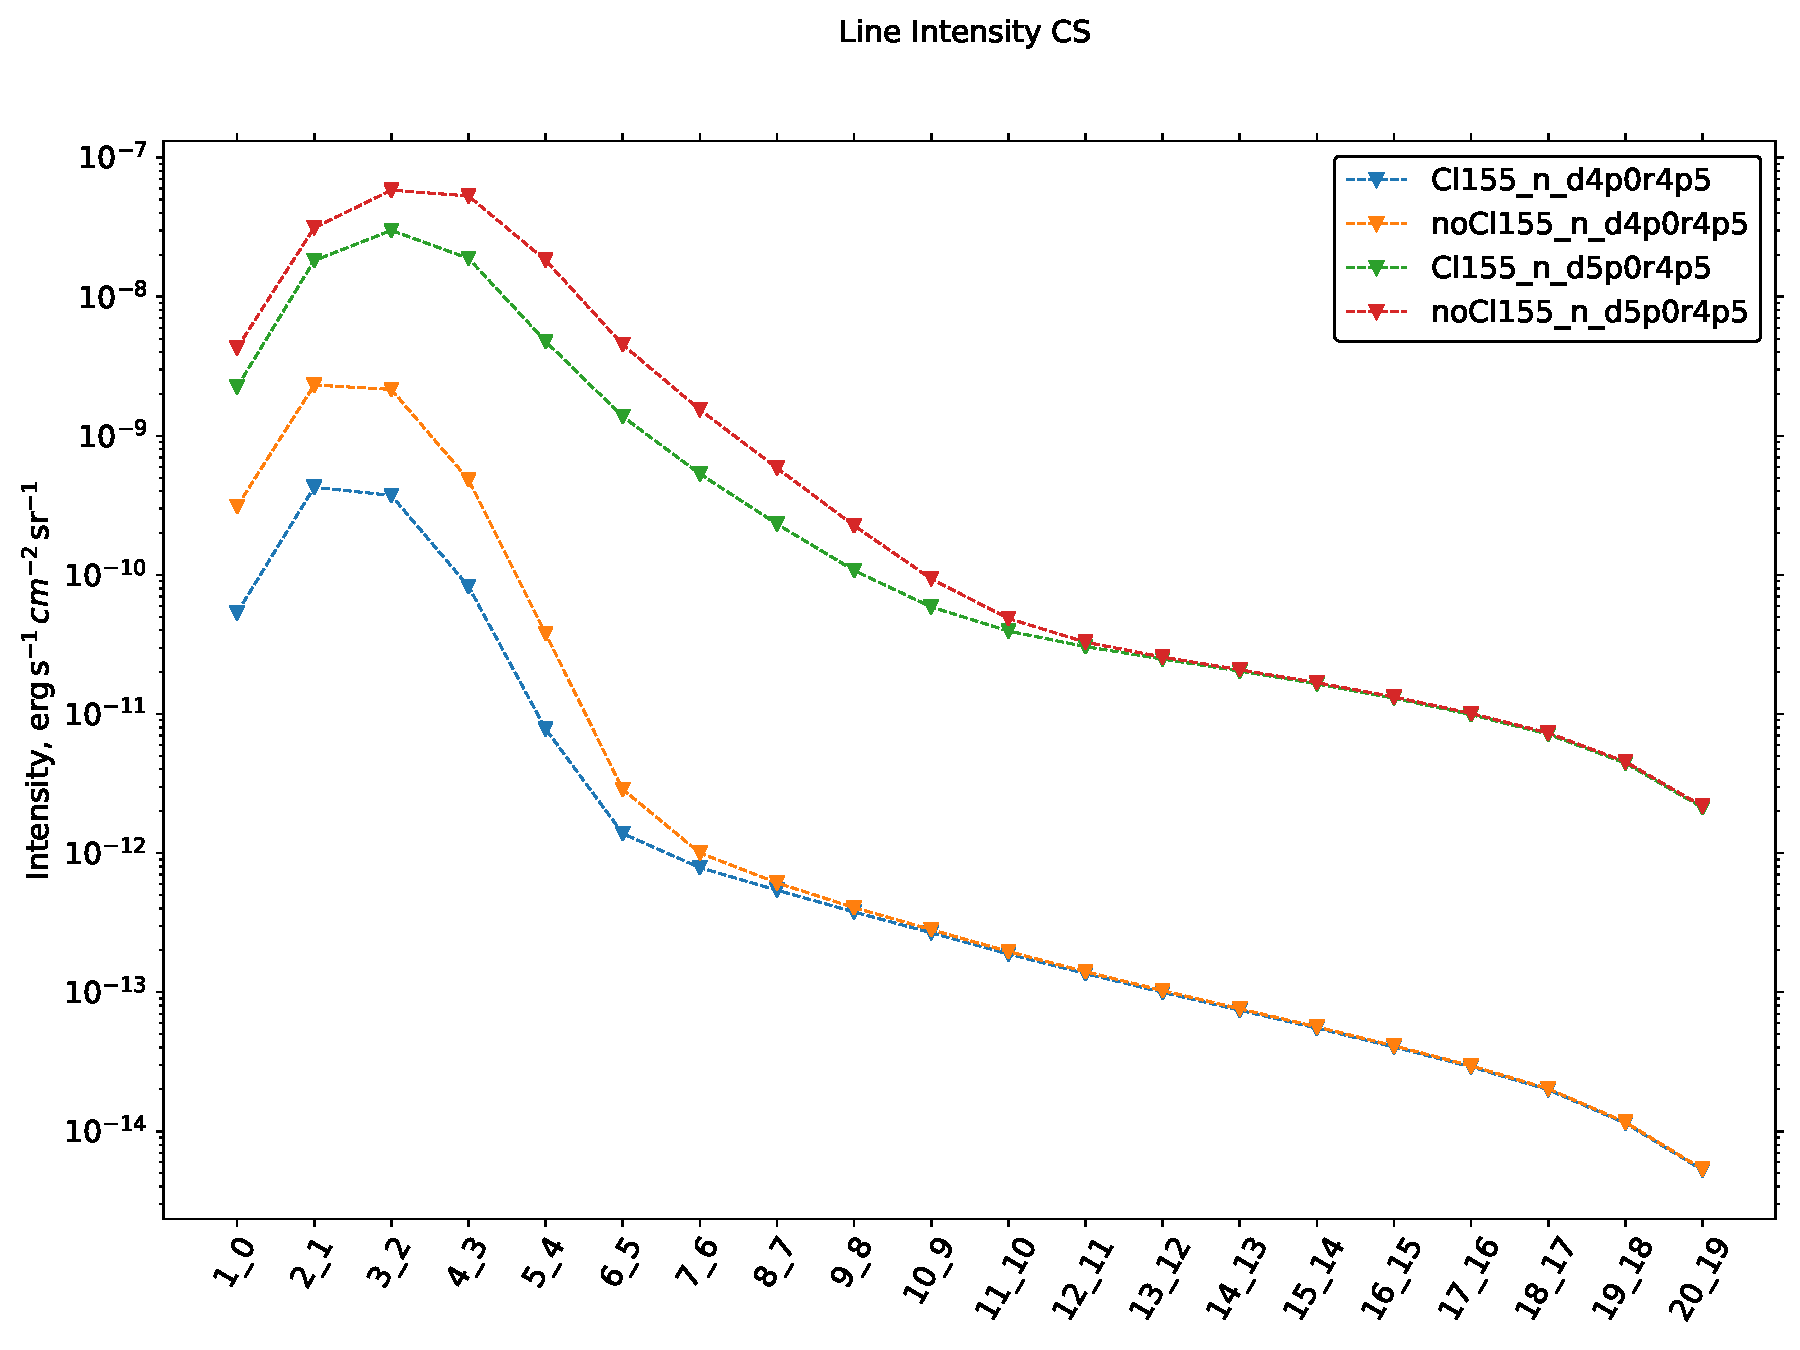
\includegraphics[trim = {0 0 0 1.5cm},clip,width=1\textwidth]{figure/Cl/gridModelEmiss/I_comp_CS.pdf}
        \caption{$\mathrm{CS}$}
    \end{subfigure}
    ~ 
   \begin{subfigure}[t]{0.45\textwidth} % "0.45" donne ici la largeur de l'image
        \centering 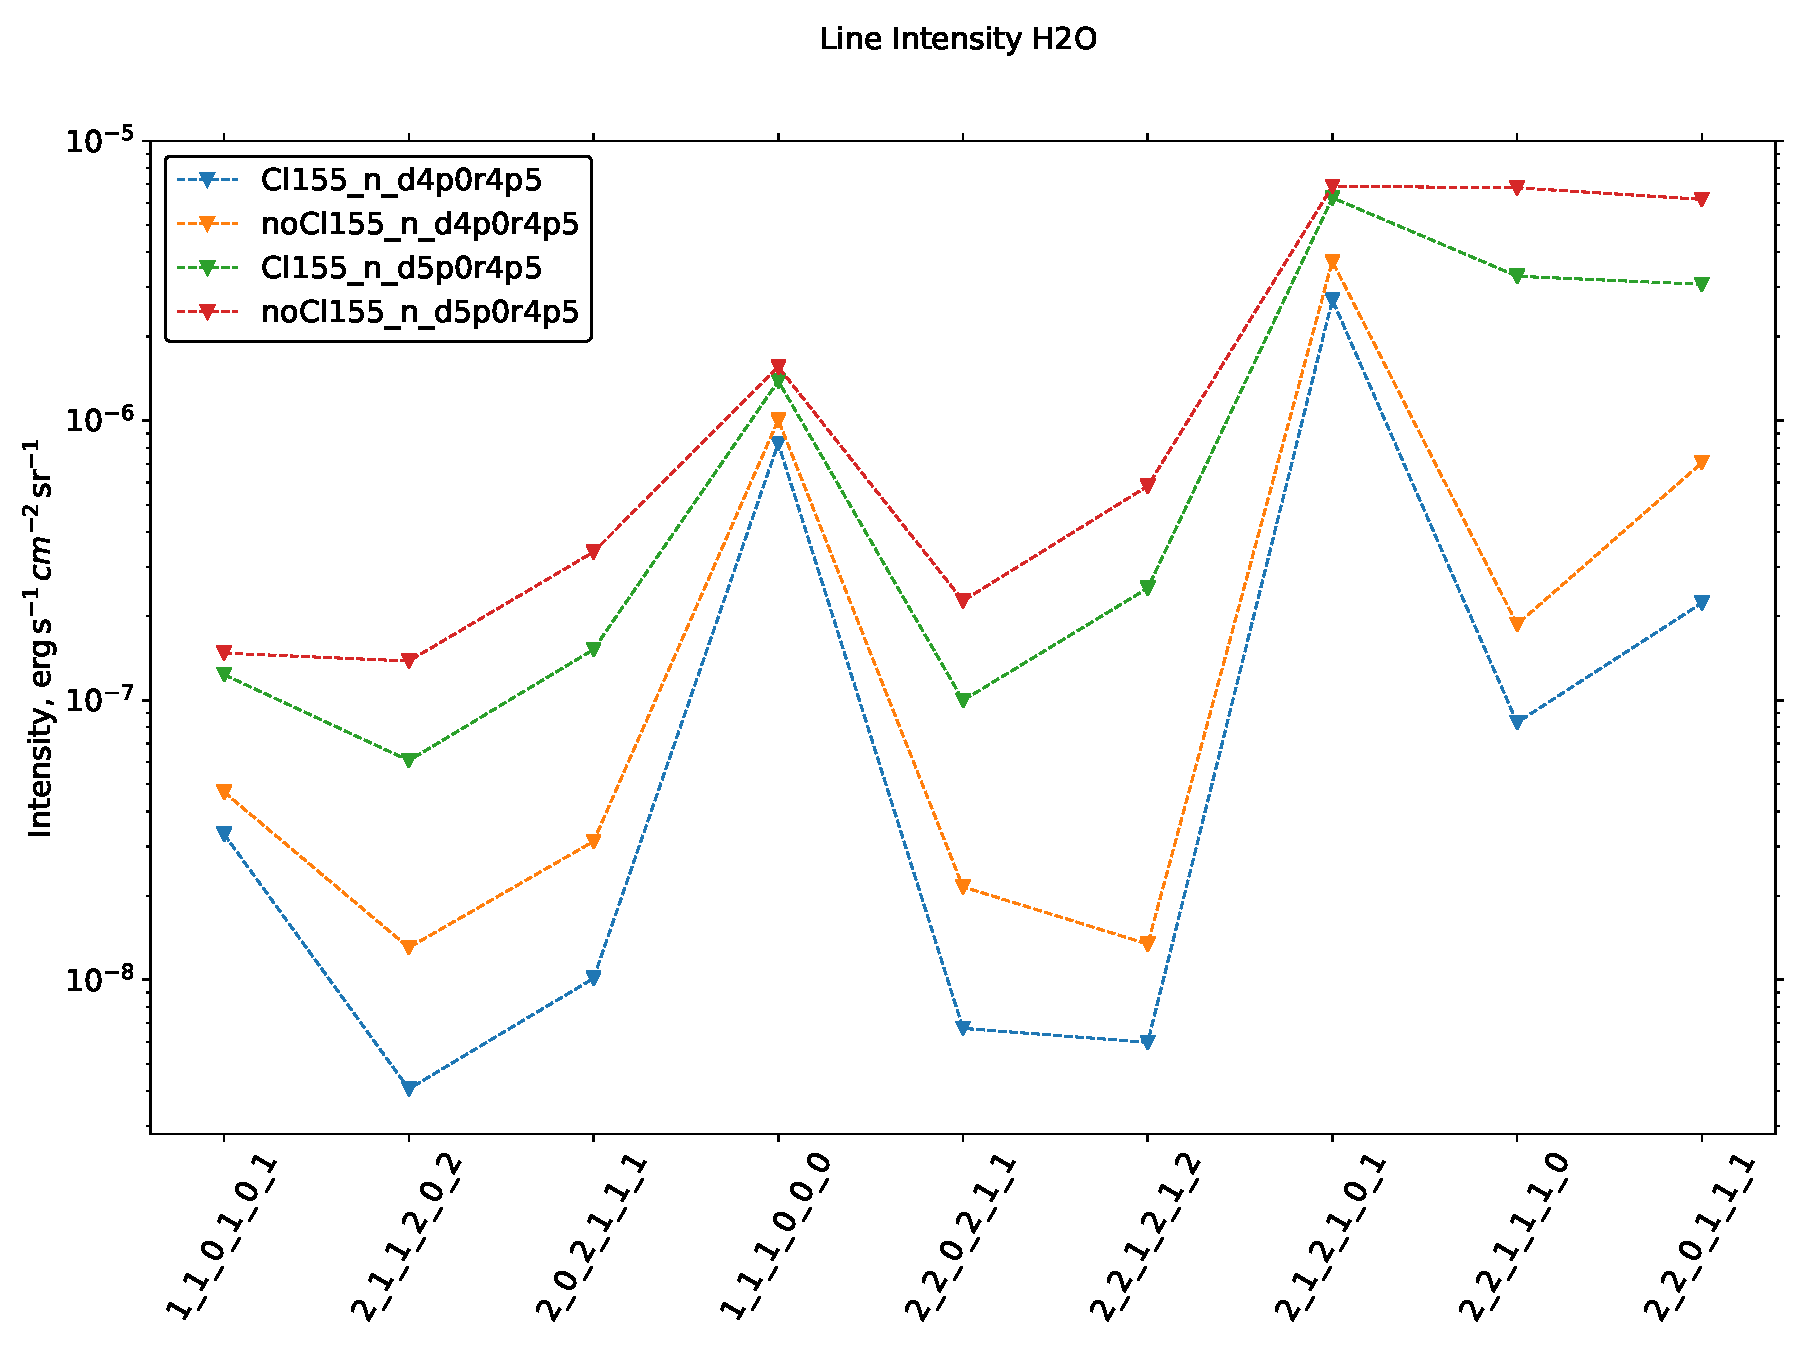
\includegraphics[trim = {0 0 0 1.5cm},clip,width=1\textwidth]{figure/Cl/gridModelEmiss/I_comp_H2O.pdf}
        \caption{$\mathrm{H}_2\mathrm{O}$}
    \end{subfigure}
    
    \begin{subfigure}[t]{0.45\textwidth} % "0.45" donne ici la largeur de l'image
        \centering 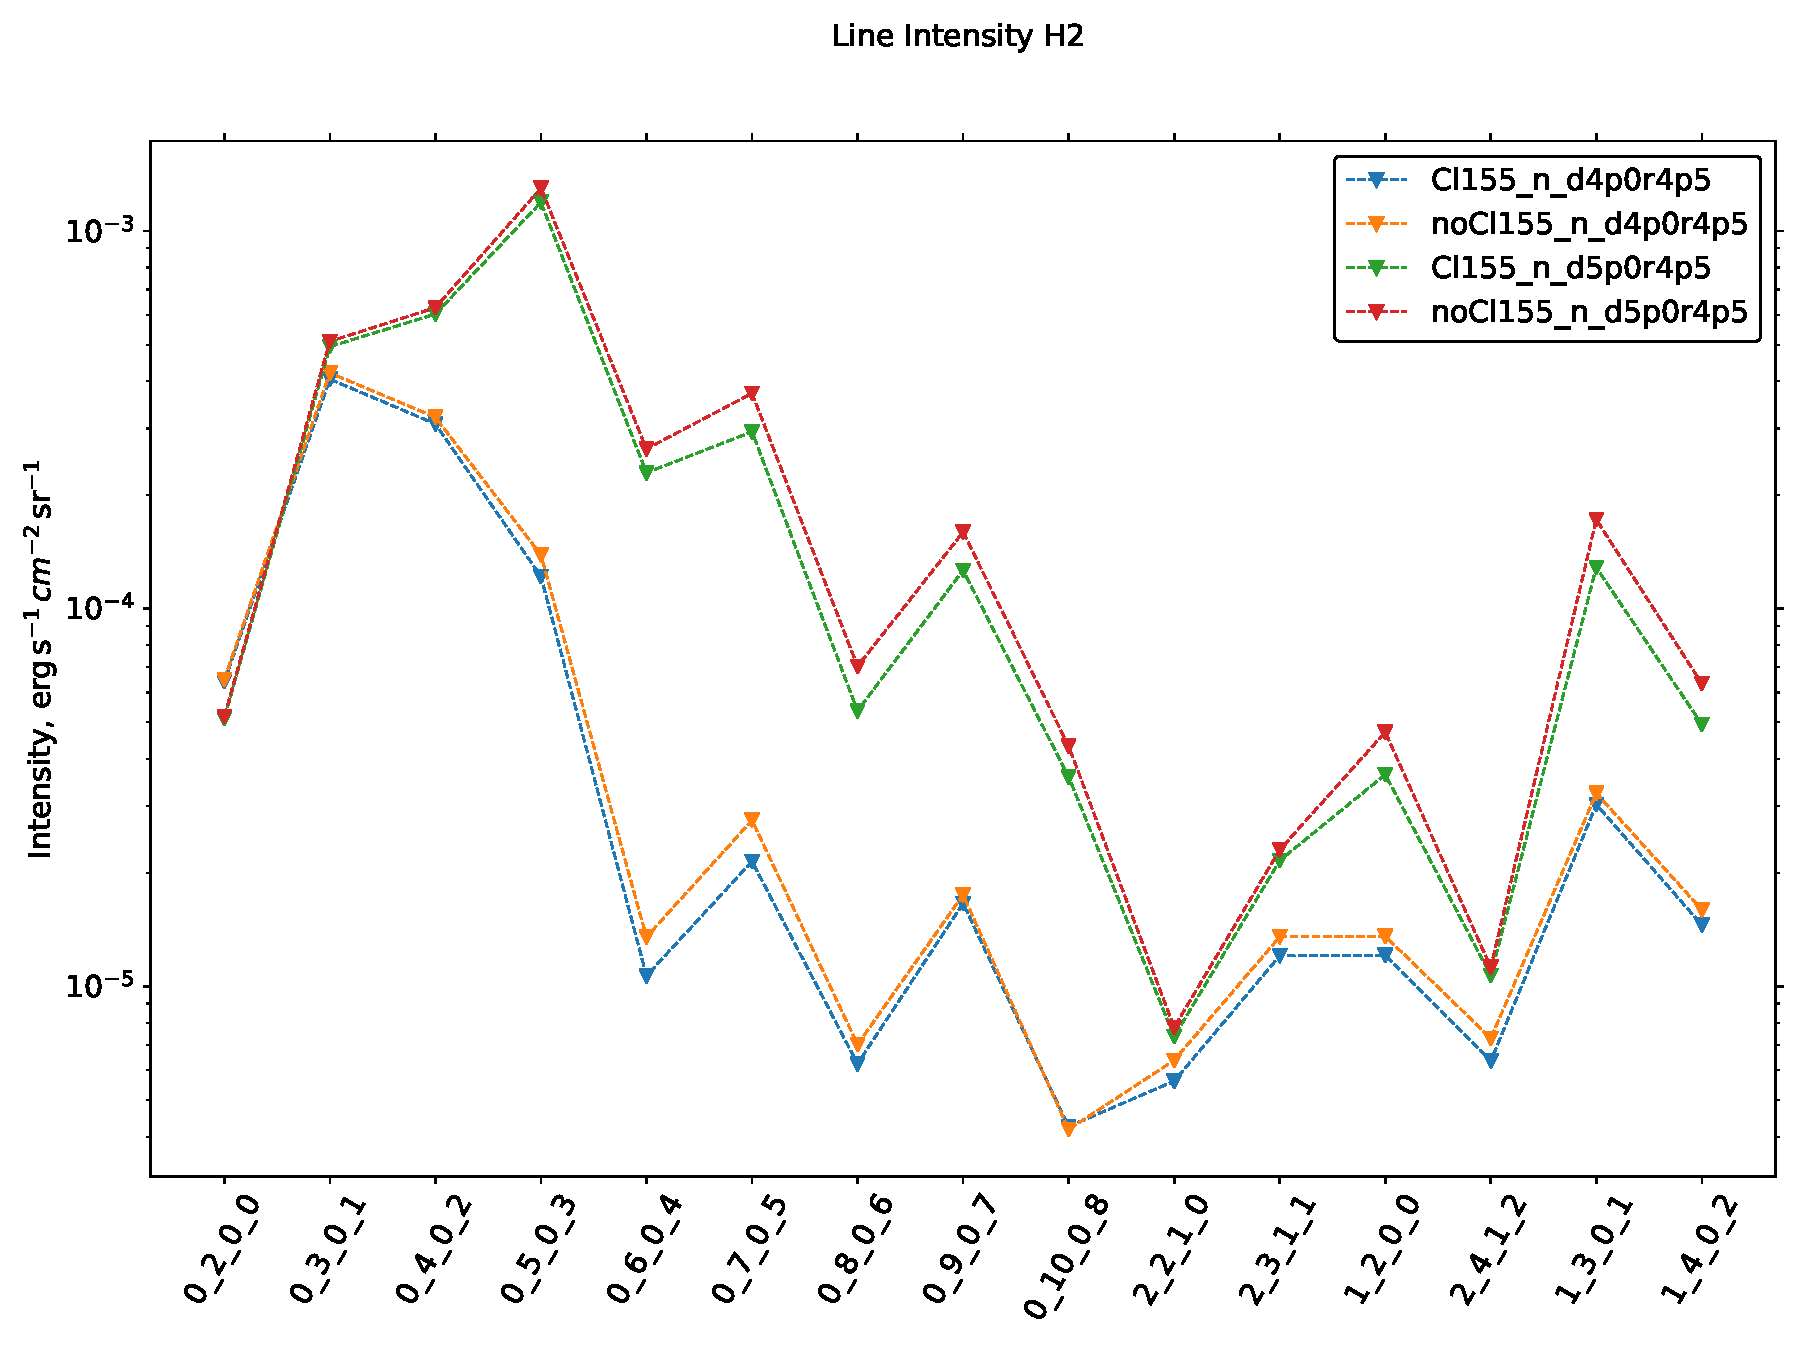
\includegraphics[trim = {0 0 0 1.5cm},clip,width=1\textwidth]{figure/Cl/gridModelEmiss/I_comp_H2.pdf}
        \caption{$\mathrm{H}_2$}
    \end{subfigure}
    ~ 
    \begin{subfigure}[t]{0.45\textwidth} % "0.45" donne ici la largeur de l'image
        \centering 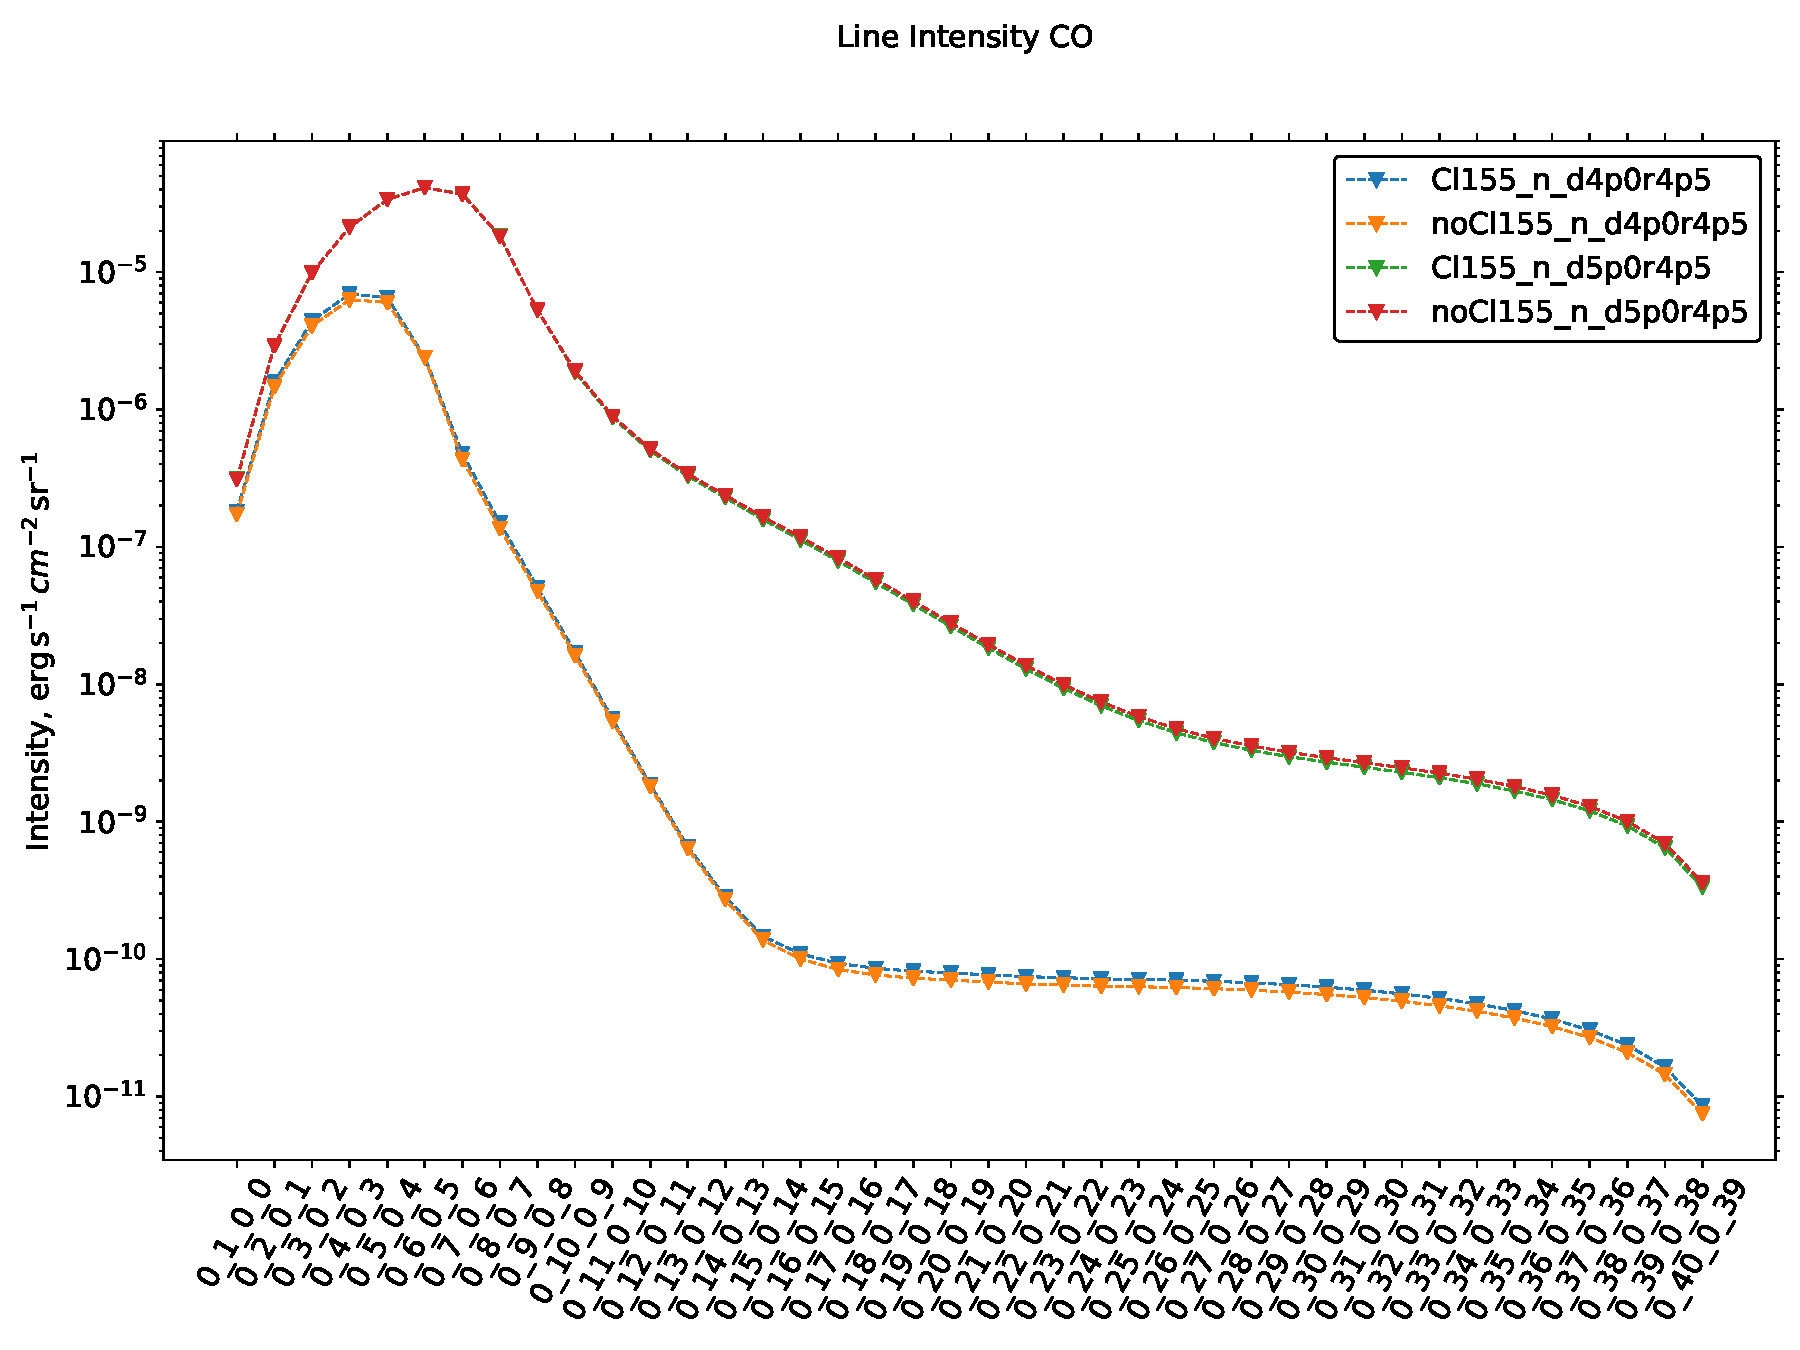
\includegraphics[trim = {0 0 0 1.5cm},clip,width=1\textwidth]{figure/Cl/gridModelEmiss/I_comp_CO.pdf}
        \caption{$\mathrm{CO}$}
    \end{subfigure}
    
    \caption{Diagramme d'excitation des traceurs peu modifiés par l'ajout du chlore dans le code PDR (\uncinq)}
    \label{fig:Cl:gridModelEmiss:no}
\end{figure}


\subsubsection{Profils de densités des traceurs}

Pour comprendre les changements causé par le chlore sur les raies des traceurs, on a tracé les profils de densités et températures des traceurs dans le nuage figures \ref{fig:Cl:gridModelEmiss:nT:yes} et \ref{fig:Cl:gridModelEmiss:nT:no}. On remarque que pour le $\mathrm{N}$, la densité en bord atomique, reste identique tandis que pour le $\mathrm{N}^+$, $\mathrm{S}$ et $\mathrm{Si}$ leurs densités augmentent d'un facteur $\times 2$ à $\times 6$ en plus de l'augmentation de température. Ces raies seraient excités principalement dans les bords atomiques de la PDR et sont touché par l'ajout du chlore. Les autres espèces ($\mathrm{CS}$, $\mathrm{H}_2\mathrm{O}$, $\mathrm{H}_2$ et $\mathrm{CO}$) ne semblent pas impacté par le chlore (hormis $\mathrm{CS}$ d'un facteur $\times 2$. \newline 

Attention, on voit les profils s'effondrer à partir de $A_\mathrm{V} \geq 4$ qui est du à un défaut du code dans le cas des modèles à densités constantes qui ne peut plus calculer la formation de $\mathrm{H}_2$ au sein du nuage moléculaire. 

\begin{figure}[!htbp]
    \centering
    \begin{subfigure}[t]{0.45\textwidth} % "0.45" donne ici la largeur de l'image
        \centering 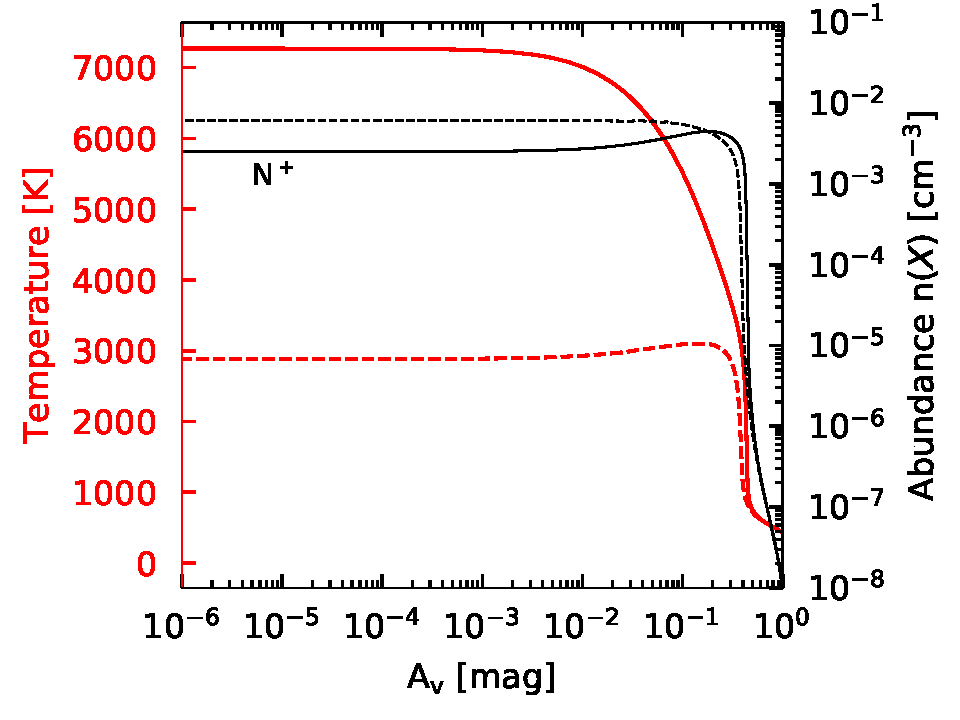
\includegraphics[trim = {0 0 0 1.5cm},clip,width=1\textwidth]{figure/Cl/gridModelEmiss/nT_comp_Np.pdf}
        \caption{$\mathrm{N}^+$}
    \end{subfigure}
    ~ 
   \begin{subfigure}[t]{0.45\textwidth} % "0.45" donne ici la largeur de l'image
        \centering 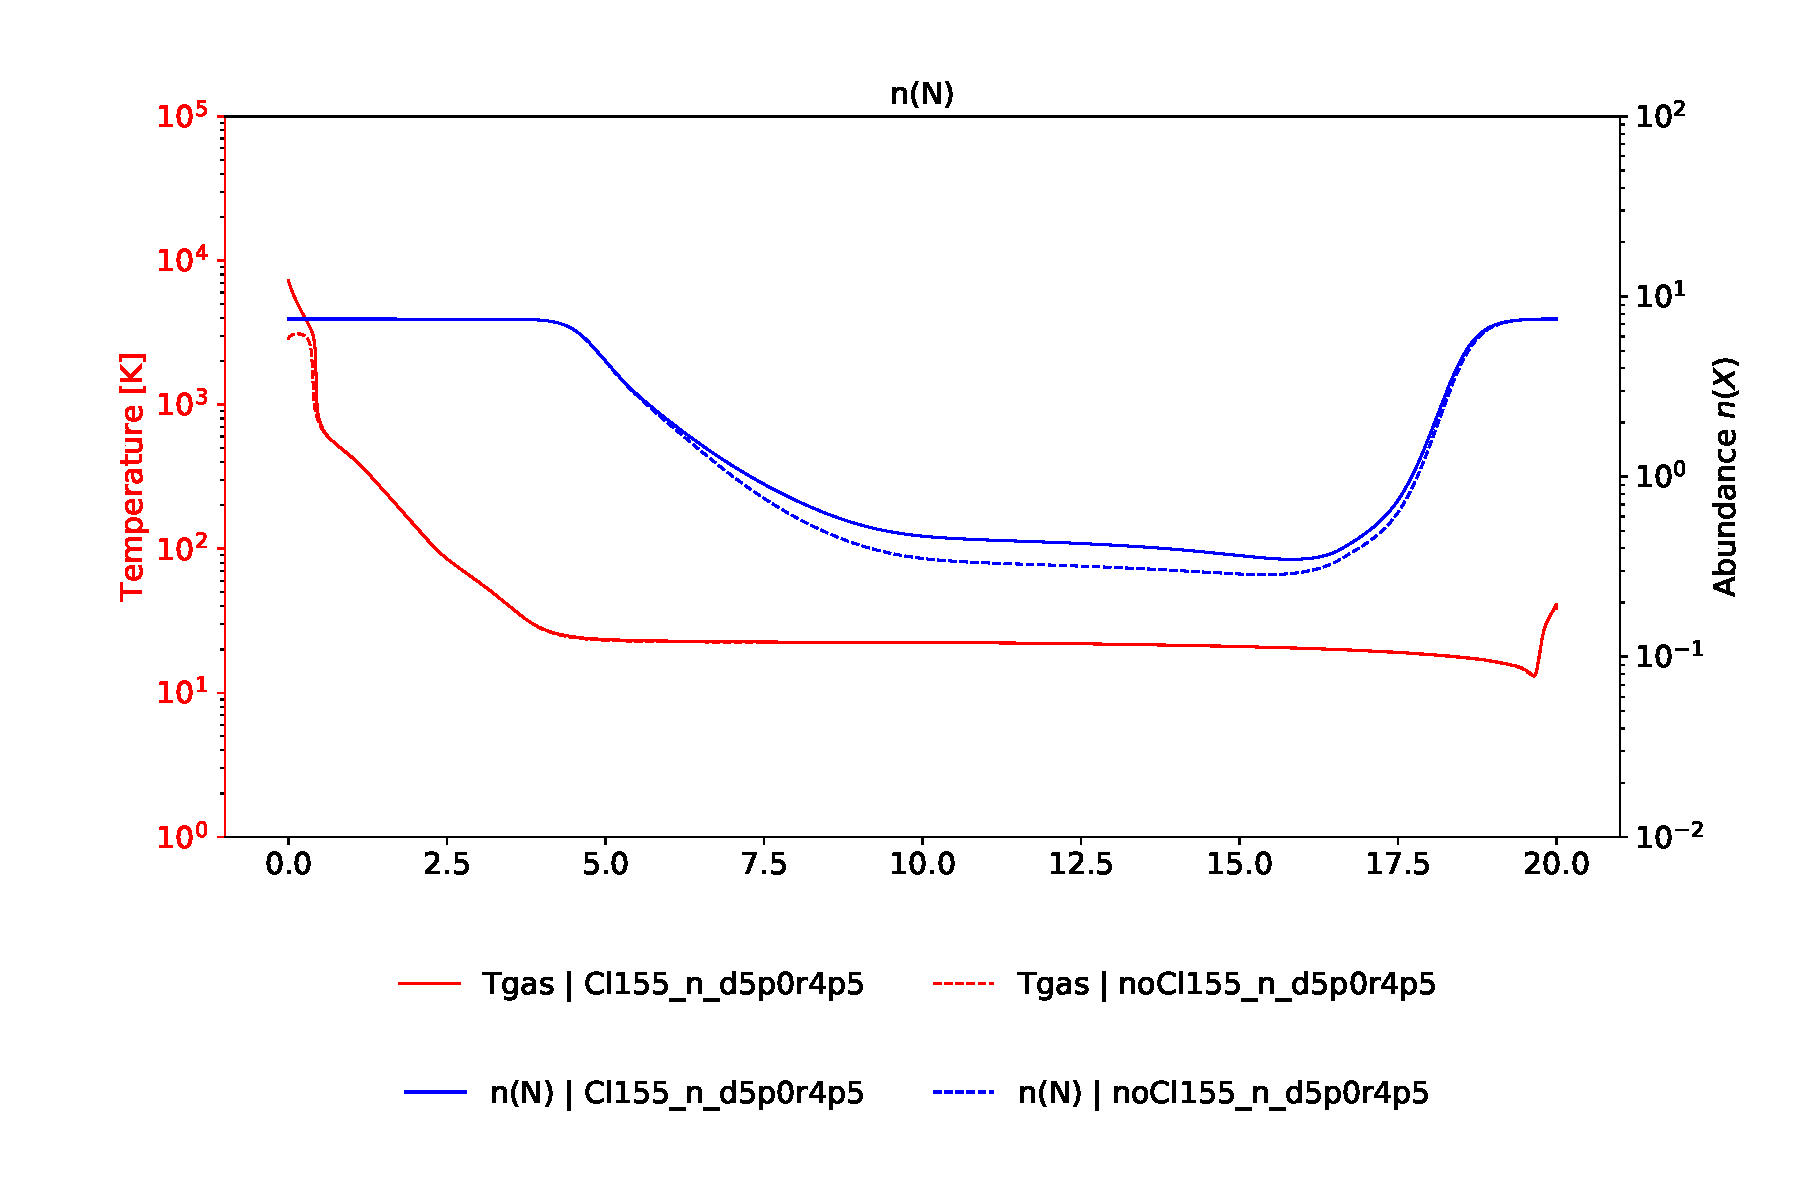
\includegraphics[trim = {0 0 0 1.5cm},clip,width=1\textwidth]{figure/Cl/gridModelEmiss/nT_comp_N.pdf}
        \caption{$\mathrm{N}$}
    \end{subfigure}
    
    \begin{subfigure}[t]{0.45\textwidth} % "0.45" donne ici la largeur de l'image
        \centering 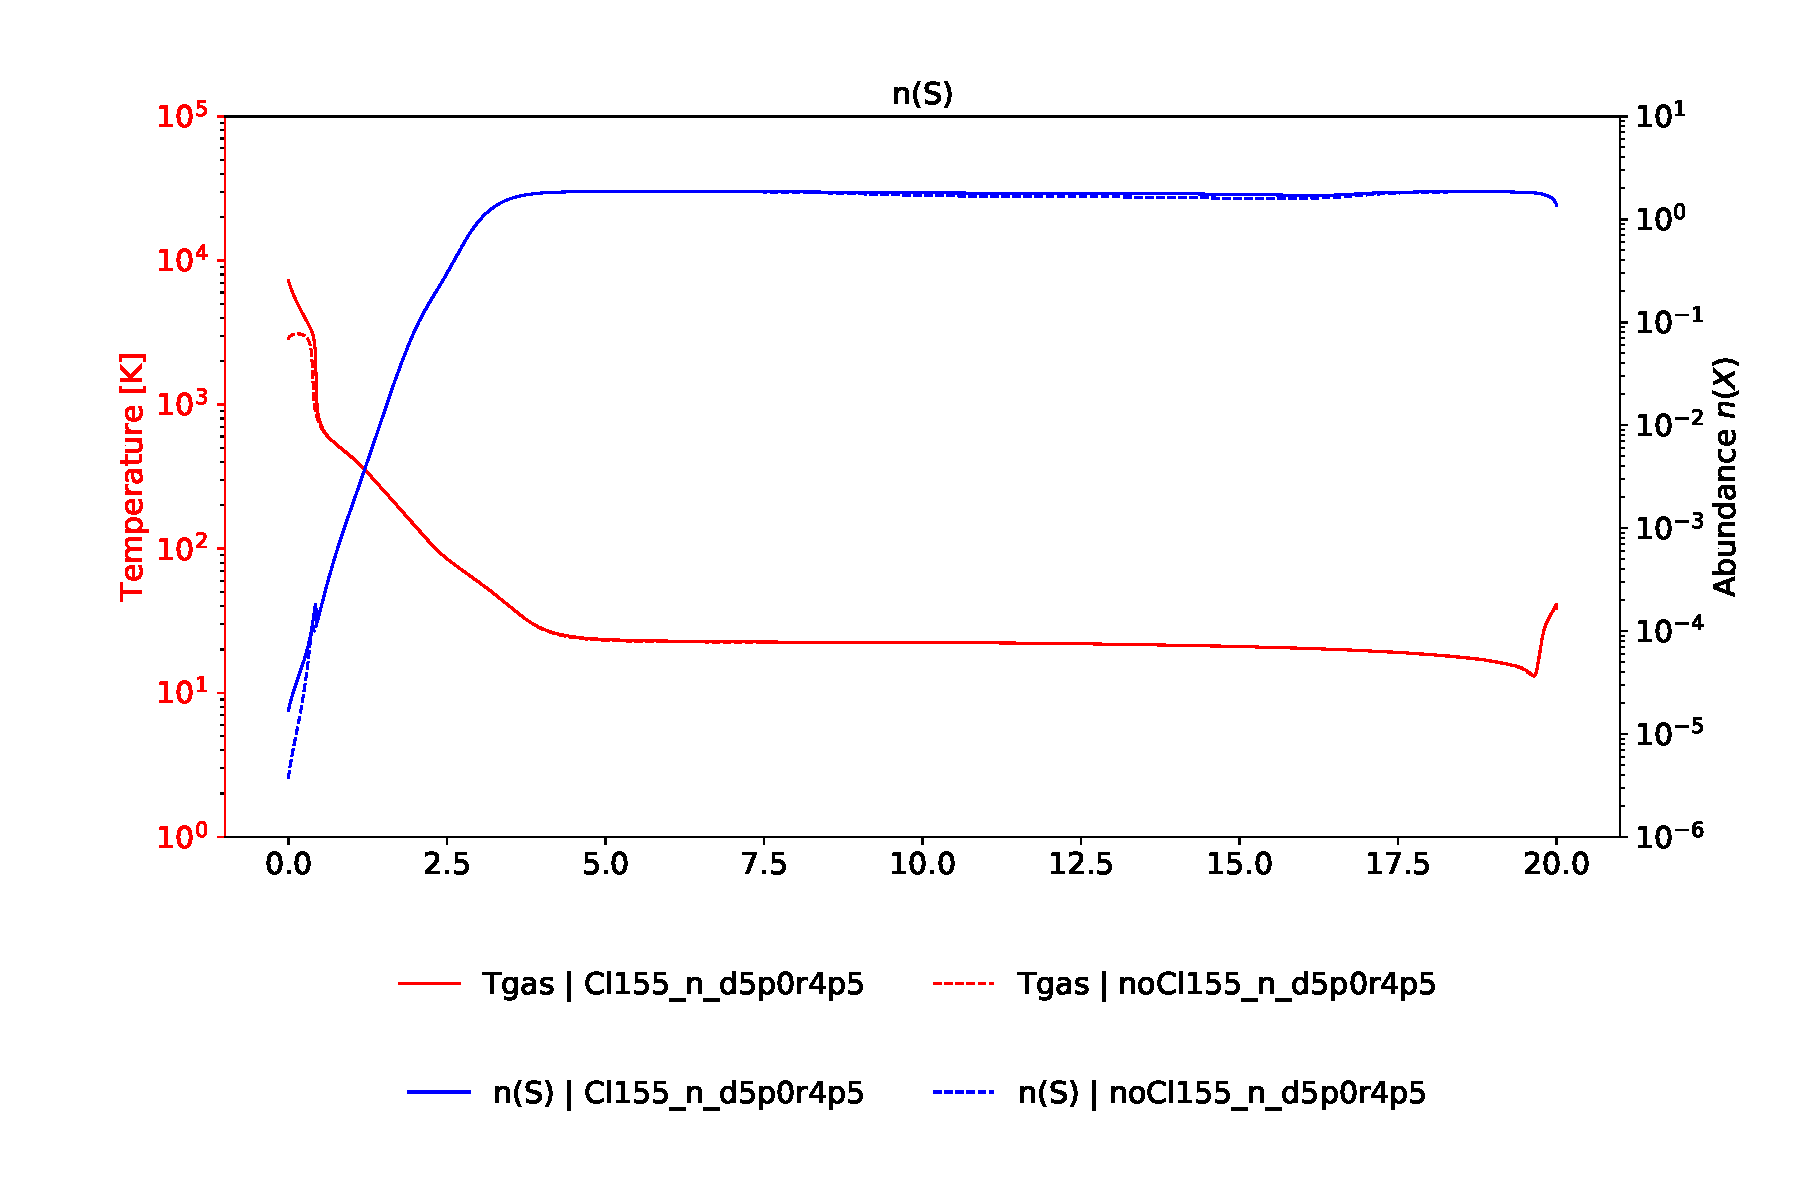
\includegraphics[trim = {0 0 0 1.5cm},clip,width=1\textwidth]{figure/Cl/gridModelEmiss/nT_comp_S.pdf}
        \caption{$\mathrm{S}$}
    \end{subfigure}
    ~
    \begin{subfigure}[t]{0.45\textwidth} % "0.45" donne ici la largeur de l'image
        \centering 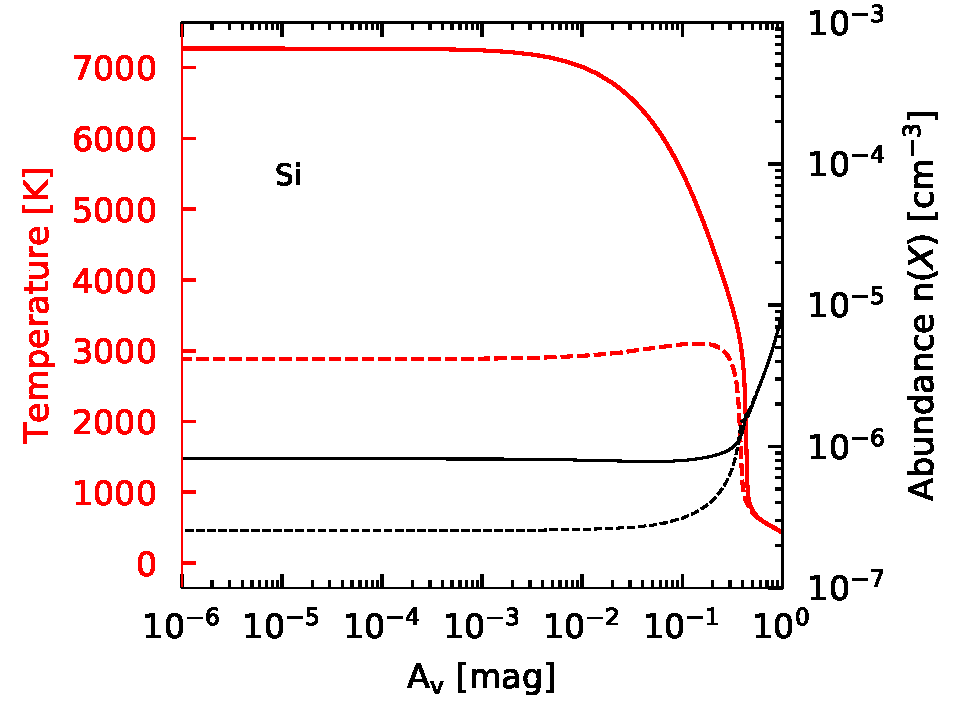
\includegraphics[trim = {0 0 0 1.5cm},clip,width=1\textwidth]{figure/Cl/gridModelEmiss/nT_comp_Si.pdf}
        \caption{$\mathrm{Si}$}
    \end{subfigure}
    
    \caption{Profils de densité des traceurs modifiés par l'ajout du chlore dans le code PDR (\uncinq)}
    \label{fig:Cl:gridModelEmiss:nT:yes}
\end{figure}

\begin{figure}[!htbp]
    \centering
    \begin{subfigure}[t]{0.45\textwidth} % "0.45" donne ici la largeur de l'image
        \centering 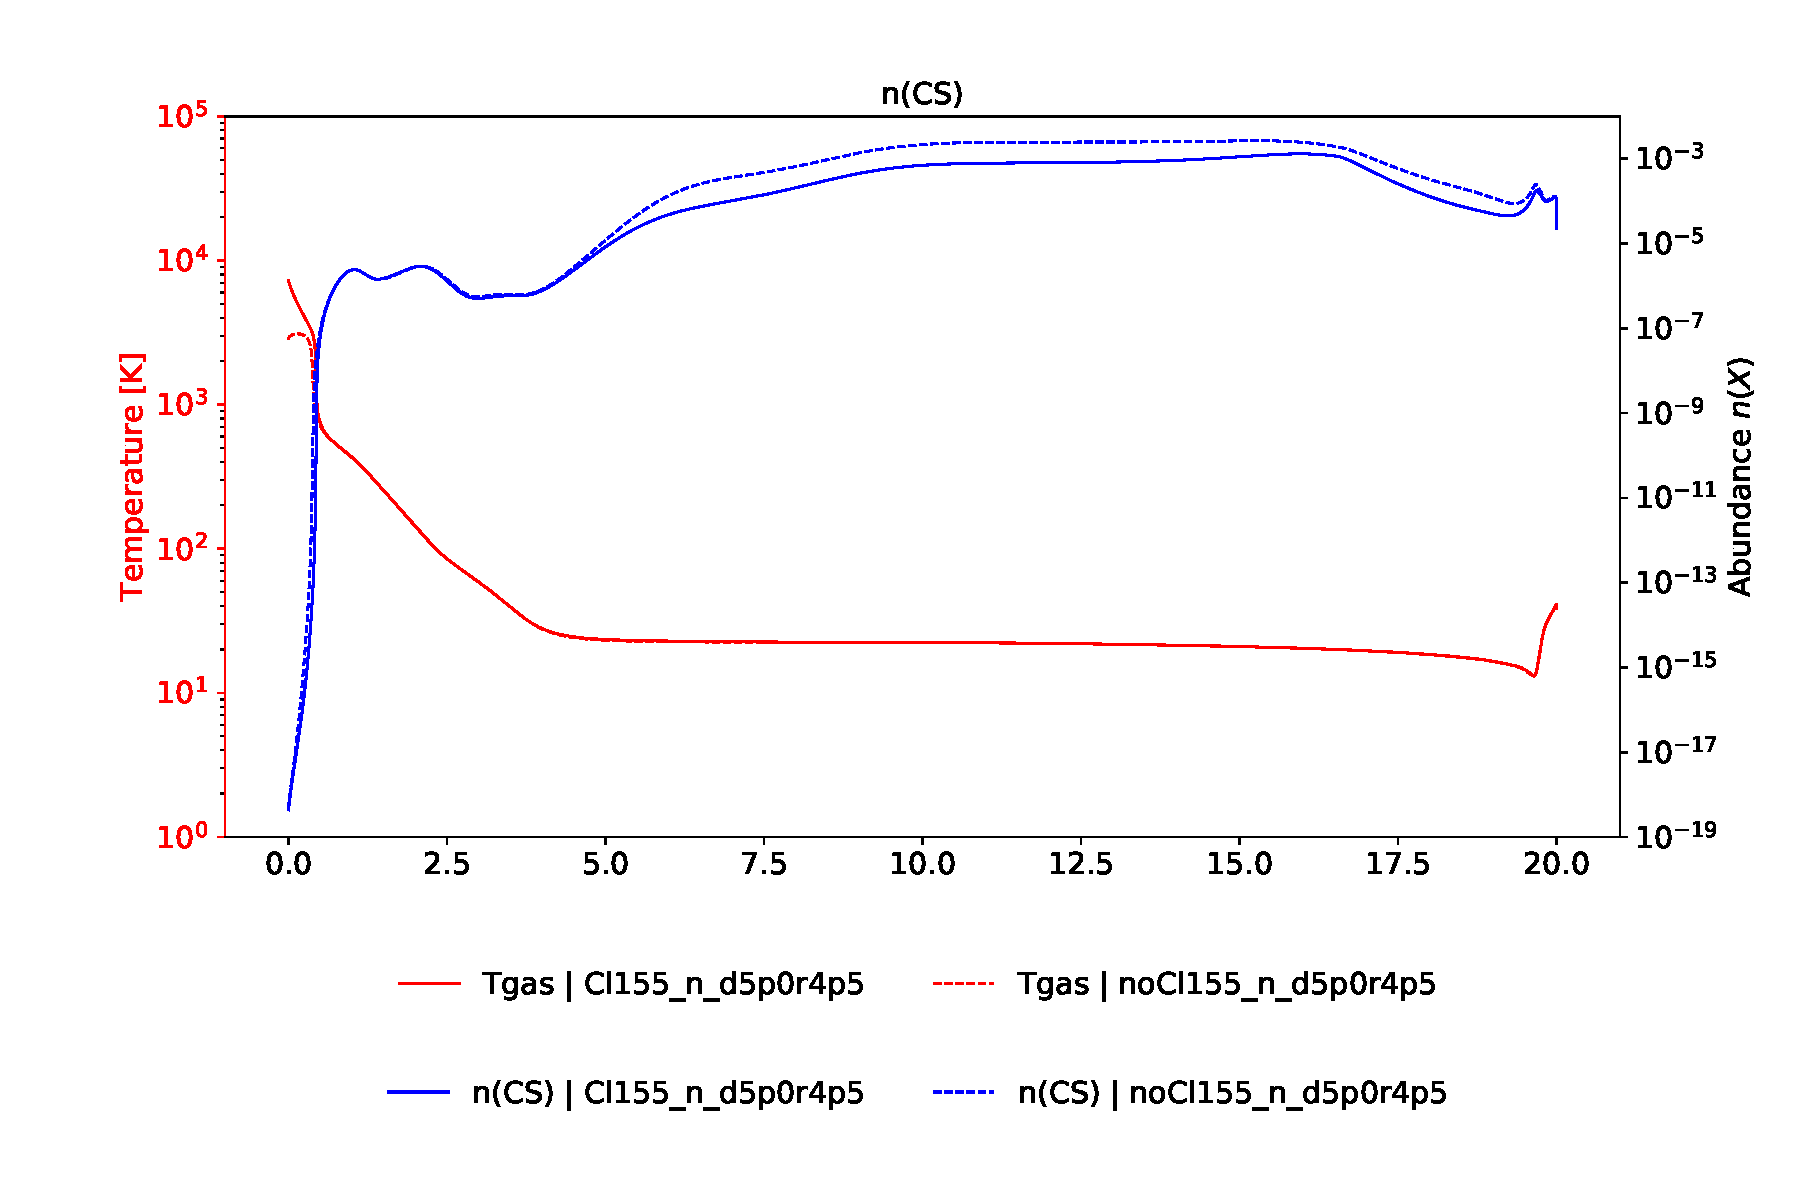
\includegraphics[trim = {0 0 0 1.5cm},clip,width=1\textwidth]{figure/Cl/gridModelEmiss/nT_comp_CS.pdf}
        \caption{$\mathrm{CS}$}
    \end{subfigure}
    ~ 
   \begin{subfigure}[t]{0.45\textwidth} % "0.45" donne ici la largeur de l'image
        \centering 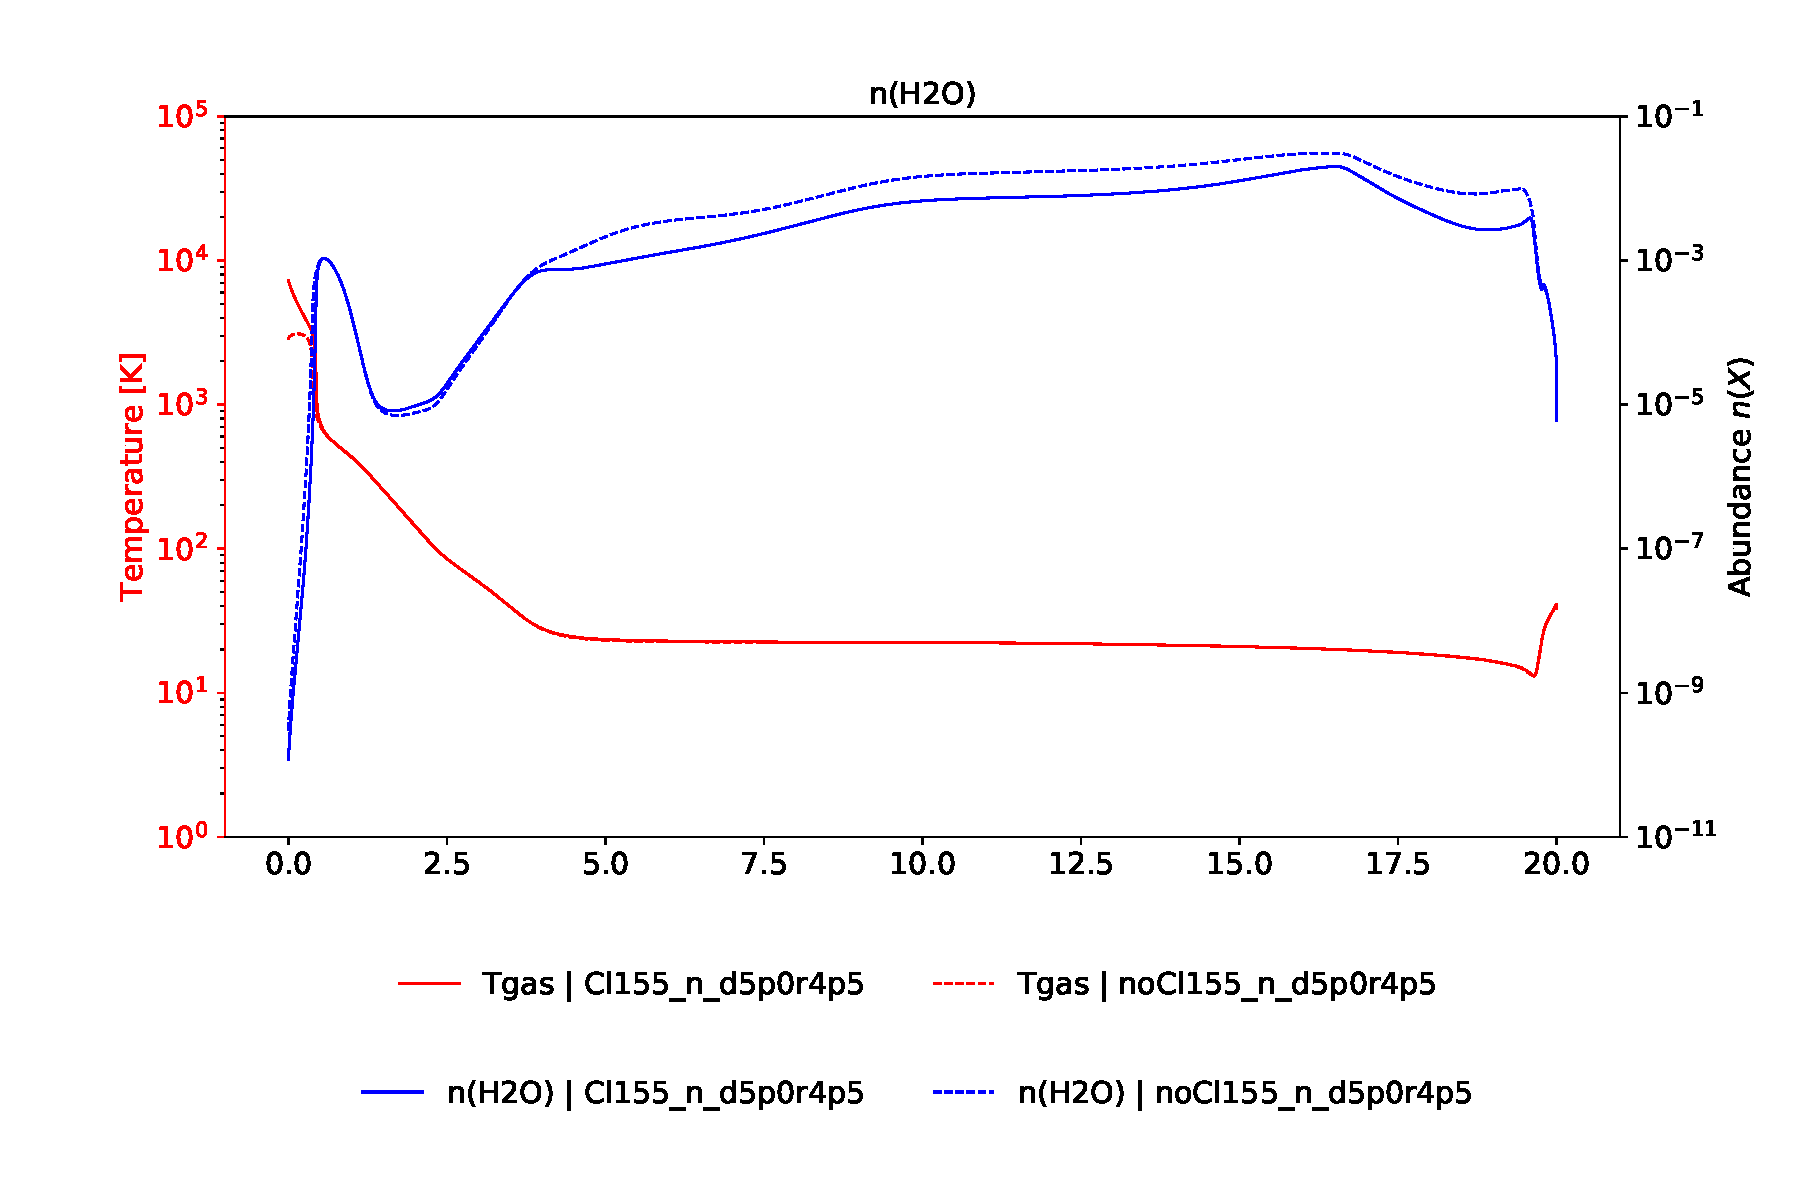
\includegraphics[trim = {0 0 0 1.5cm},clip,width=1\textwidth]{figure/Cl/gridModelEmiss/nT_comp_H2O.pdf}
        \caption{$\mathrm{H}_2\mathrm{O}$}
    \end{subfigure}
    
    \begin{subfigure}[t]{0.45\textwidth} % "0.45" donne ici la largeur de l'image
        \centering 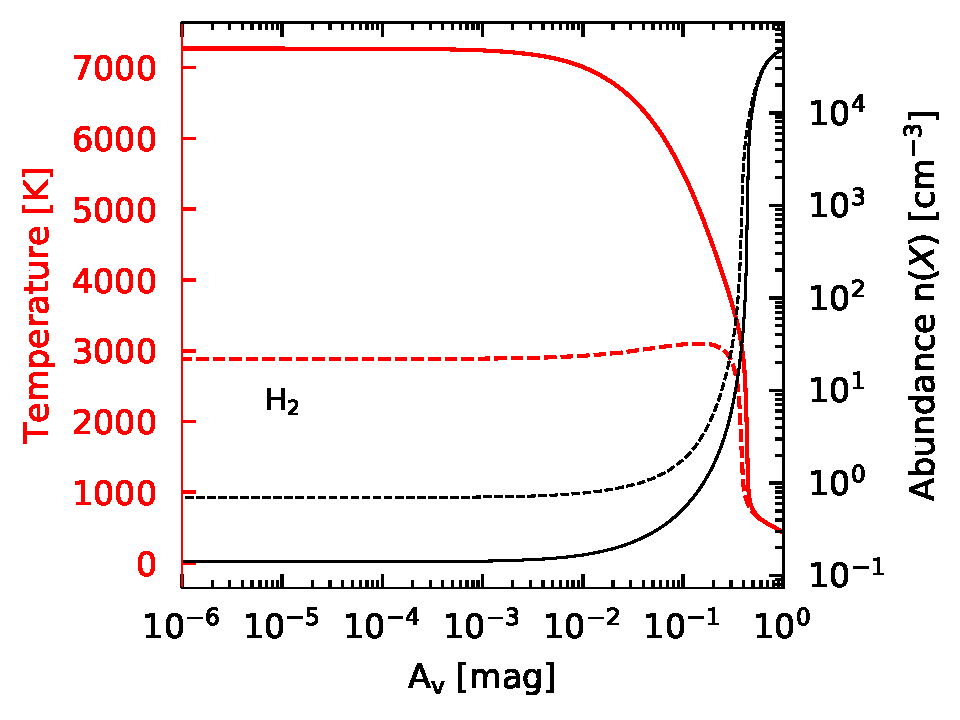
\includegraphics[trim = {0 0 0 1.5cm},clip,width=1\textwidth]{figure/Cl/gridModelEmiss/nT_comp_H2.pdf}
        \caption{$\mathrm{H}_2$}
    \end{subfigure}
    ~ 
    \begin{subfigure}[t]{0.45\textwidth} % "0.45" donne ici la largeur de l'image
        \centering 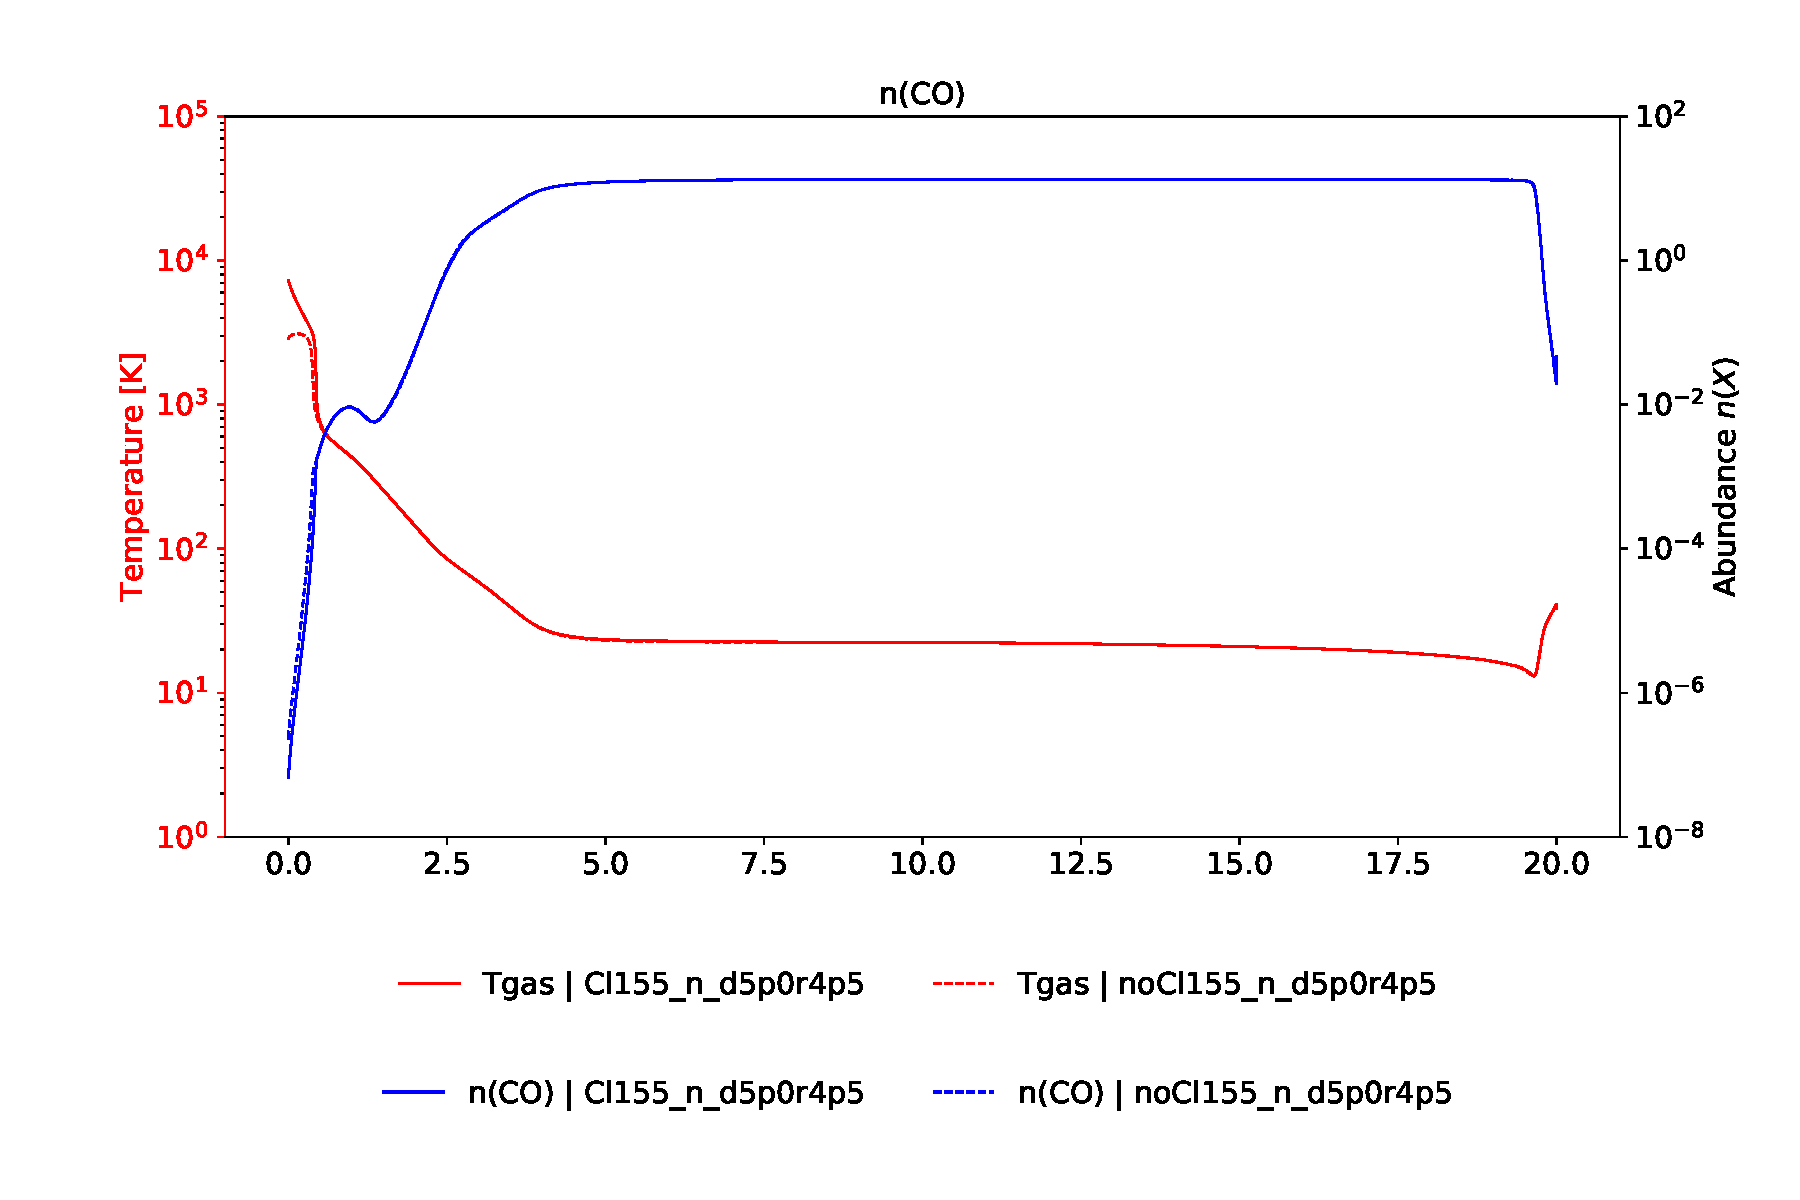
\includegraphics[trim = {0 0 0 1.5cm},clip,width=1\textwidth]{figure/Cl/gridModelEmiss/nT_comp_CO.pdf}
        \caption{$\mathrm{CO}$}
    \end{subfigure}
    
    \caption{Profil des densités des traceurs peu modifiés par l'ajout du chlore dans le code PDR (\uncinq)}
    \label{fig:Cl:gridModelEmiss:nT:no}
\end{figure}

\subsubsection{Cartes d'intensité}

Les raies que l'on espère pouvoir observer doivent être intenses (supérieur à un "seuil" d'observabilité $\sim 10^{-6} \ \mathrm{erg}\,\mathrm{cm}^{-2}\,\mathrm{s}^{-1}$), sensible l'ajout du chlore et appartenir aux domaines de longueurs d'ondes observées. La raie la plus prometteuse est la raie [N]$5200.257 \mathrm{A}$ correspondant à la transition (El=2Do,J=5/2)$\rightarrow$(El=4So,J=3/2). On voit sur la figure \ref{fig:Cl:gridModelEmiss:N} que lorsque l'on a du chlore, l'intensité de la raie atteint est de l'ordre de $10^{-3} \mathrm{erg}\,\mathrm{cm}^{-2}\,\mathrm{s}^{-1}$ et que l'on a une signature de la solution chaude proposée par le chlore. Néanmoins la taille de la zone concernée est petite et il est difficile de bien situer les observations dans l'espace des paramètres. Un autre problème, qui n'est pas des moindres, est que les modèles de PDR commencent après la partir ionisé de l'hydrogène et que le potentiel de ionisation de l'azote est de $14.6 \ \mathrm{eV}$ ce qui signifie que la transition $\mathrm{N}^+/\mathrm{N}$ se fait devant le nuage. Dans le code, l'azote est excité par collision avec les espèces majoritaires du nuage qui sont $\mathrm{H}$,$\mathrm{H}^+$ $\mathrm{H}_2$, $\mathrm{He}$ et $e^-$. La fraction électronique en bord atomique de nuage, dans le cas d'un emballement lié au chlore, est d'un facteur $10^{-4}$-$10^{-3}$ alors qu'il est d'un facteur 1 dans la partie ionisé du nuage. Cette augmentation de l'intensité de la raie sera masqué par le front $\mathrm{N}^+/\mathrm{N}$. \newline

Il faudrait donc trouver des traceurs qui ont des potentiels de ionisations inférieures à celui de l'hydrogène et qui s'activerait uniquement en bord atomique. Enfin on a tracé les diagrammes d'excitations avec des modèles à densités constantes qui sont peut efficaces pour corroborer avec les données. Il faudrait lancer des grilles isobares et voir ce qu'il en est.


\begin{figure}[!htbp]
    \centering
    \begin{subfigure}[t]{0.45\textwidth} % "0.45" donne ici la largeur de l'image
        \centering 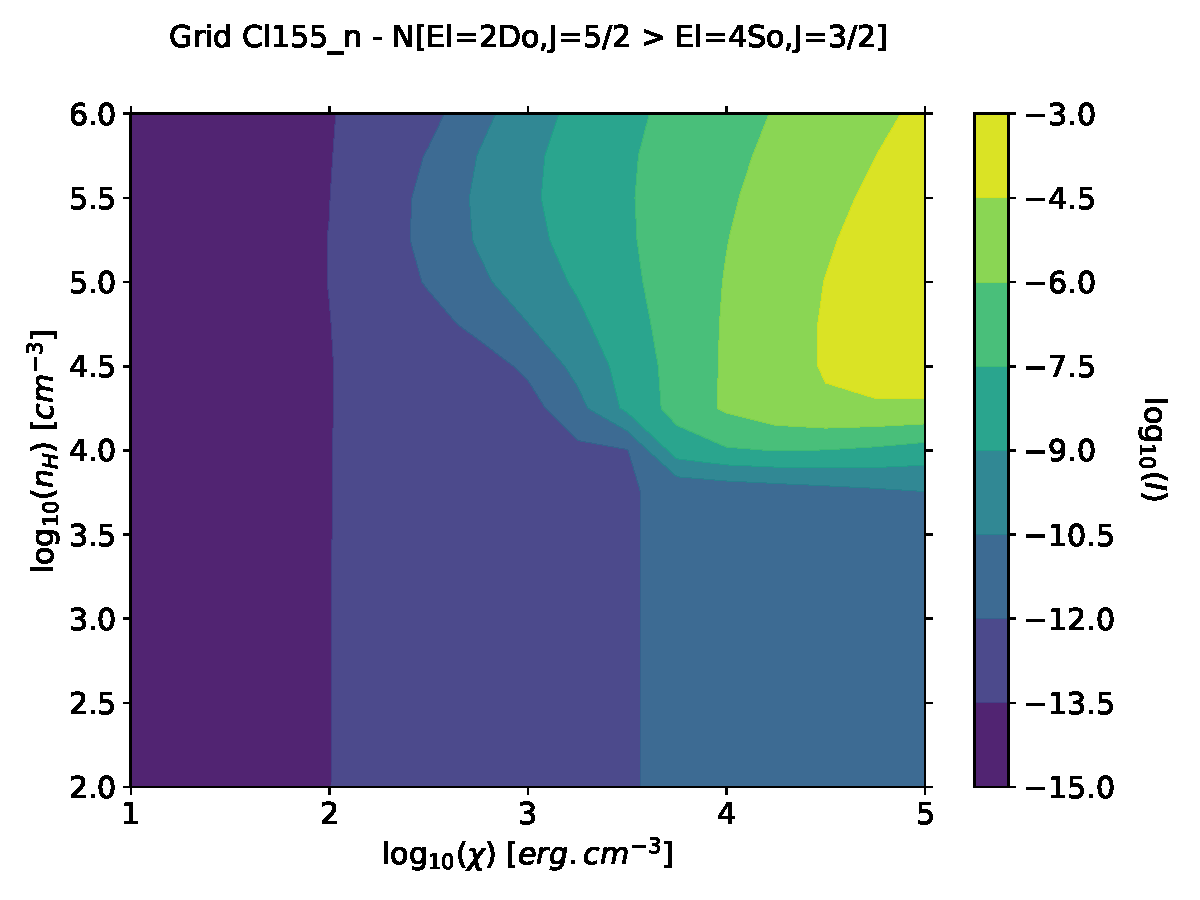
\includegraphics[trim = {0 0 0 1.5cm},clip,width=1\textwidth]{figure/Cl/gridModelEmiss/mapI_N.pdf}
        \caption{Emissivité de la raie [N]$5200.257 \mathrm{A}$ d'une grille de modèle avec Chlore.}
    \end{subfigure}
    ~ 
    \begin{subfigure}[t]{0.45\textwidth} % "0.45" donne ici la largeur de l'image
        \centering 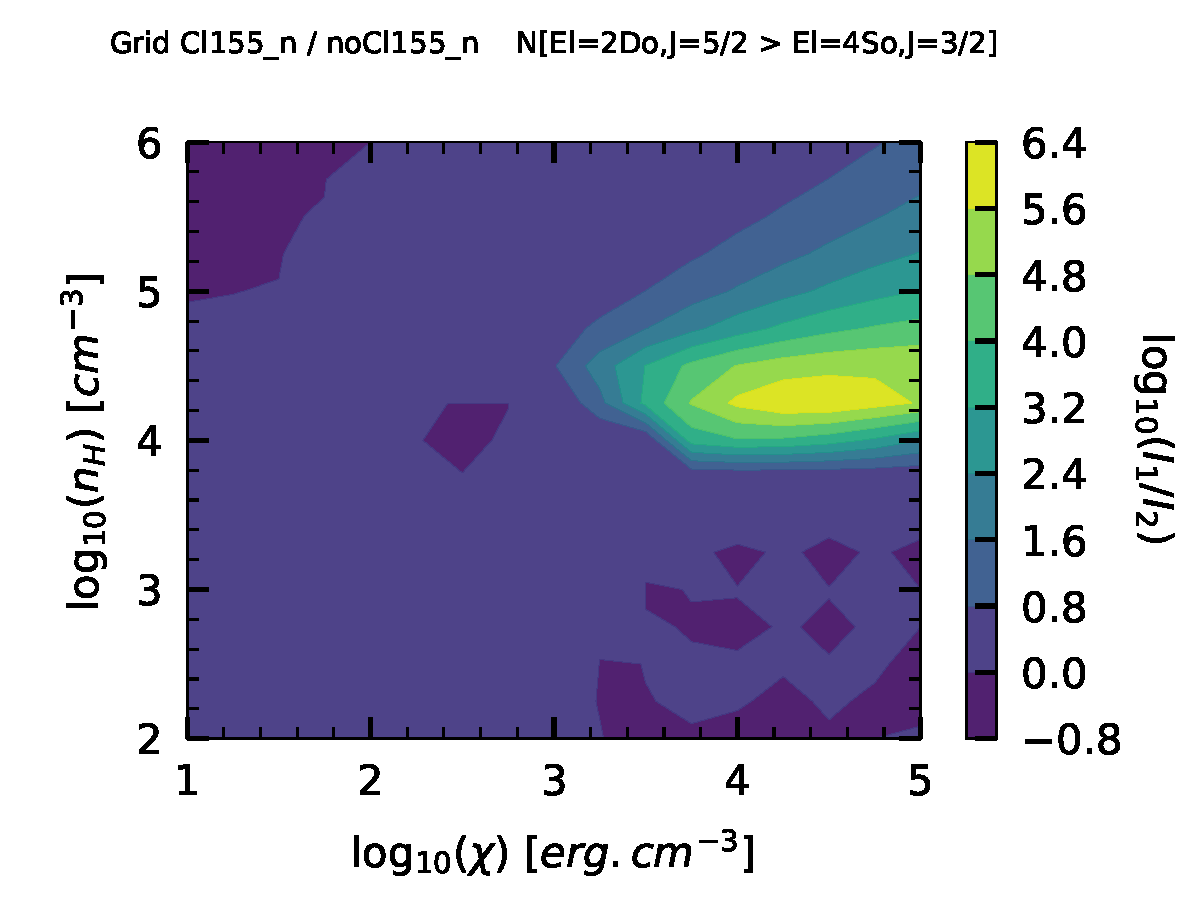
\includegraphics[trim = {0 0 0 1.5cm},clip,width=1\textwidth]{figure/Cl/gridModelEmiss/map_Cl155_n_noCl155_nI_N.pdf}
        \caption{Rapport des émissivités dans le cas avec ou sans chlore des grilles de modèles}
    \end{subfigure}
    
    \caption{}
    \label{fig:Cl:gridModelEmiss:N}
\end{figure}


%%%%%%%%%%%%%%%%%%%%%%%%%%%%%%%%%%%%%%%%%%%%%%%%%%%%%%%%%%%%%%%%%%%%%%%%%%%%%%%%%%%%%%%%%%%%%%%

\subsection{Comparaison avec le modèle}


\section{Réduction de l'énergie d'activation des réactions avec $\mathrm{H}_2$}


Dans certaines zones du nuage, une fraction importante de $\mathrm{H}_2$ est excitée par pompage UV dans ses états vibrationnels. Pour les réactions impliquant la molécule, une partie de l'énergie nécessaire à la réaction peut être prélevée dans son énergie interne ce qui a tendance à les favoriser. La prise en compte de l'énergie interne de la molécule a un impact sur les intensités des raies d'émissions de traceurs clés comme le $\mathrm{CO}$ \cite{COJoblin}, $\mathrm{H}_2$ ou $\mathrm{H}_2\mathrm{O}$. C'est un phénomène déjà bien connu pour la formation du $\mathrm{CH}^+$ (eq \ref{eq:C++H2}) \cite{Herraez, Zanchet}.

\begin{equation} \label{eq:C++H2}
    \begin{array}{lllclll}
        \mathrm{C}^+ & + &\mathrm{H}_2   & \rightarrow &\mathrm{CH}^+  & + & \mathrm{H} \\
    \end{array}
\end{equation}

Pour calculer le nouveau taux de réaction, le principe est de passer de la loi d'Arrhénius à un calcul des taux de réactions entre chaque populations des niveaux du $\mathrm{H}_2$ et de l'espèce $\mathrm{X}$. Cependant réaliser un calcul précis de ce phénomène est coûteux car il demande de connaître les taux de réactions d'une espèce avec la molécule $\mathrm{H}_2$ dans chacun de ses états excités. Afin de mieux expliquer les raies d'émissions, on cherche à comprendre comment un nouveau calcul des coefficients de réaction qui prend en compte l'énergie interne de $\mathrm{H}_2$ modifie les voies de formations des principaux traceurs. Sans connaître précisément les taux des réactions des populations de $\mathrm{H}_2$ avec 
des espèces autres que le $\mathrm{C}^+$, le code PDR fait une approximation de la nouvelle prescription. Si elle entraîne des changements majeurs dans la chimie et les raies d'émissions des traceurs, il sera alors intéressant de faire un calcul précis de ces taux. \newline 

Les différences les plus importantes que l'on observe sur les spectres d'émissions sont pour la molécule du $\mathrm{CO}$ (figure \ref{fig:type46:CO}), du $\mathrm{H}_2$ (figure \ref{fig:type46:H2}) et $\mathrm{H}_2\mathrm{O}$ (figure \ref{fig:type46:H2O}). Or, on sait jusqu'à présent que le $\mathrm{CO}$ est principalement formé à partir du $\mathrm{CH}^+$ et que le calcul précis du taux de formation du $\mathrm{CH}^+$ par le $\mathrm{C}^+$ (eq. \ref{eq:C++H2}) est déjà connu dans le code. L'analyse de la chimie montre que la voie de formation du $\mathrm{CO}$ par $\mathrm{OH}$ est devenue efficace ce qui contribue à former davantage de $\mathrm{CO}$ ($\times 10$) et à intensifier ses raies. Le schéma \ref{fig:type46:form:CO} rassemble les réactions servant à former la molécule. Par ailleurs, la découverte de cette nouvelle voie de formation par $\mathrm{OH}$ est un résultat important. 

\begin{figure}[!h]
    \centering 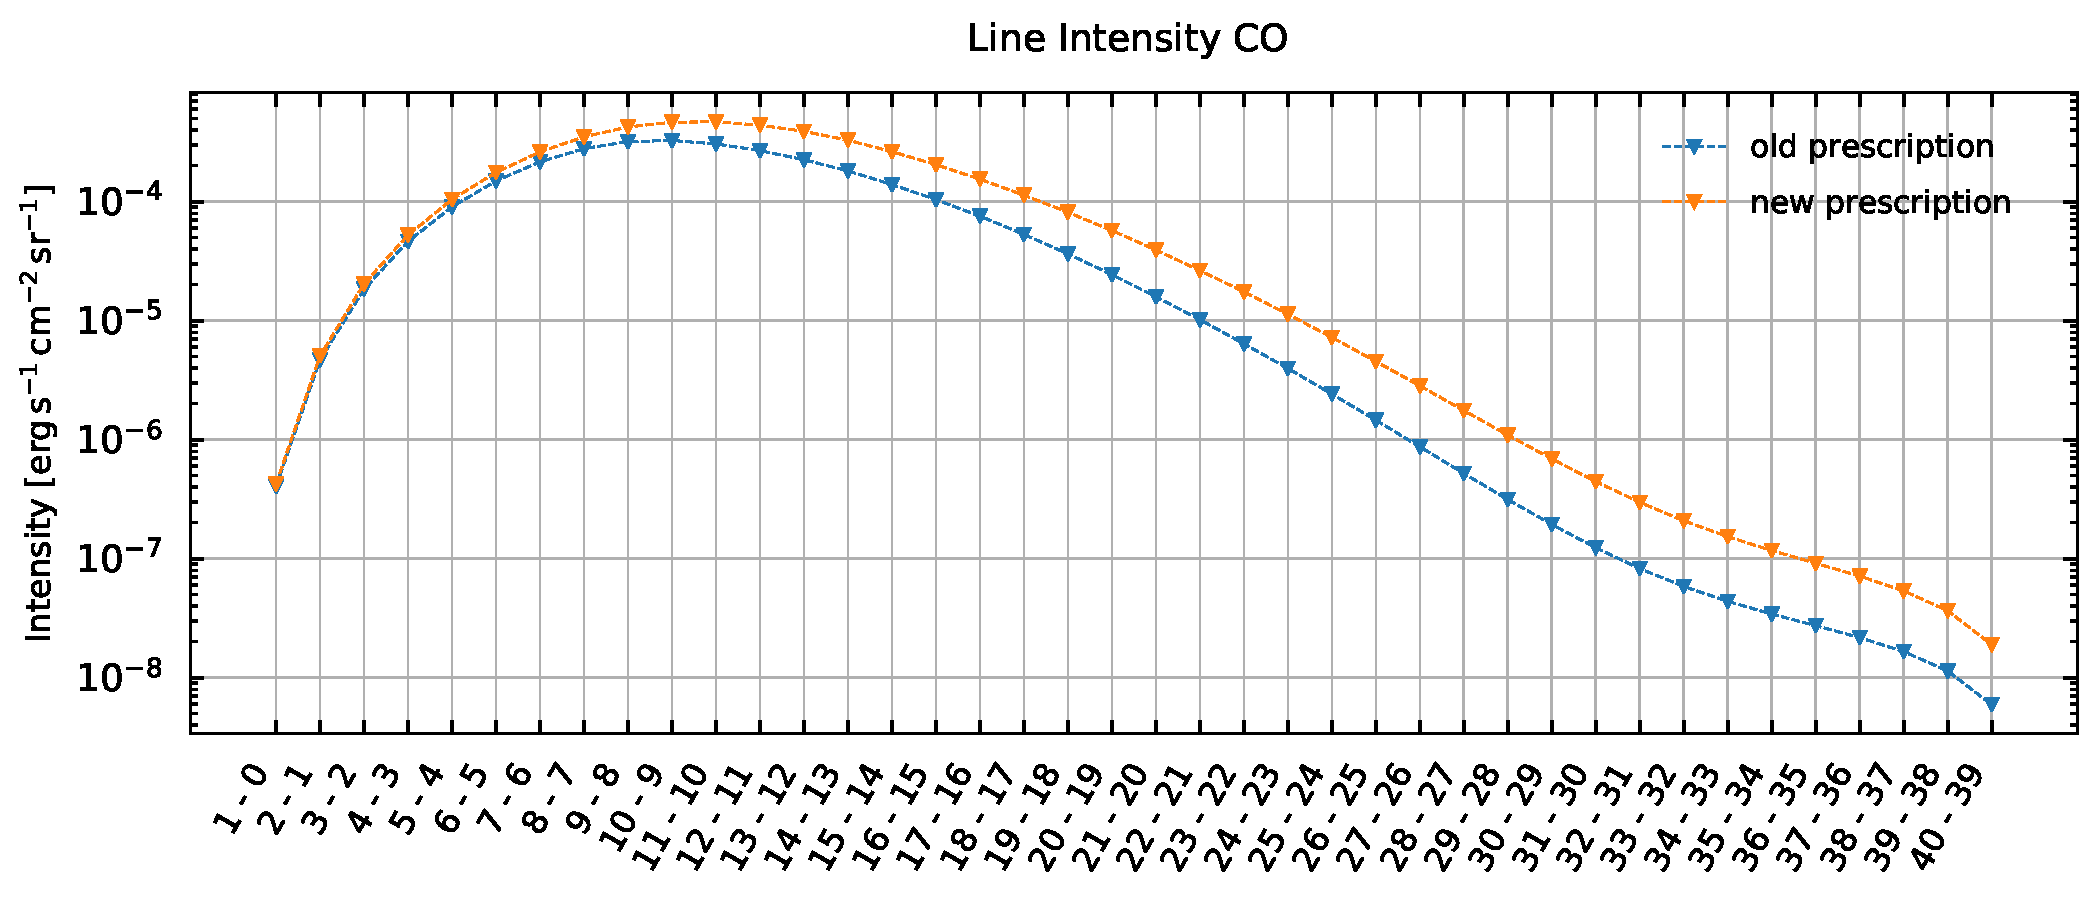
\includegraphics[trim = {0 0 0 1cm},clip,width=0.8\textwidth]{figure/type46/I_comp_CO.pdf}
    \caption{Diagramme d'intensité du $\mathrm{CO}$ avec la nouvelle prescription}
    \begin{minipage}{\textwidth}
    Seules les transitions rotationnelles du $\mathrm{CO}$ ont été écrites (toutes s'effectuent à $\mathrm{v}=0$). Un modèle isobare a été choisi ($\mathrm{P} = 2.8\,10^{8} \,\mathrm{cm}^3\,\mathrm{K}$ et $\chi = 3.1\, 10^4$).
    \end{minipage}
    \label{fig:type46:CO}
\end{figure}

\begin{figure}[!h]
    \centering \includegraphics[trim = {0 0 0 1cm},clip,width=0.8\textwidth]{}
    \caption{Réseau de formation du $\mathrm{CO}$}
    \begin{minipage}{\textwidth}
    
    \end{minipage}
    \label{fig:type46:form:CO}
\end{figure}

En comparant les réseaux chimiques du modèle avec la nouvelle prescription on trouve que la réaction $\mathrm{O} + \mathrm{H}_2 \rightarrow \mathrm{OH} +  \mathrm{H}$, devenue effiace, augmente la densité de $\mathrm{H}_2\mathrm{O}$ ($\times 10$) ainsi que ses raies d'émissions (figure \ref{fig:type46:H2O}). On constate également que la réaction $\mathrm{N} + \mathrm{H}_2 \rightarrow  \mathrm{NH} +  \mathrm{H}$ devient importante. La densité du $\mathrm{NH}$ augmente ($\times 10^3$) de même que celle du $\mathrm{HCN}$ ($\times 2$) et de $\mathrm{NO}$ ($\times 2$) <spectres du $\mathrm{NH}$ ?>. Il est présenté dans l'appendice \ref{} les voies de formations des espèces qui sont impactées par le nouveau calcul des taux de réactions.\newline 

Cette étude a permis de découvrir une nouvelle voie de formation du $\mathrm{CO}$ et de déceler d'autres espèces susceptibles de réagir avec le $\mathrm{H}_2$ comme $\mathrm{N}$. Enfin, on a montré qu'une connaissance plus fine de la chimie impliquant la molécule $\mathrm{H}_2$ pouvait avoir un impact important sur les spectres d'émissions des traceurs comme le $\mathrm{CO}$. Il serait intéressant de continuer l'étude dans ce sens en comparant par exemple d'autres PDR avec des conditions physiques différentes.


\section{Pompage UV de la molécule $\mathrm{H}_2$}


On cherche dans un premiers temps des expressions permettant d'estimer le chauffage par pompage UV de la molécule $\mathrm{H}_2$ calculé par le code. 

\subsection{Chauffage net par Rollïg (1995)}

\subsubsection{Chauffage par désexcitation collisionelle}
Eq (10) ou (C.3).

Il propose un modèle d'excitation effectif à deux niveaux au lieu d'un modèle prenant en compte les 15 premiers états vibrationels ($v\leq 15$) de la molécule. Se fonde sur Sternberg&Dalgarno (1995) et Burton (1990). Traduit l'absorption du flux de photons à un taux $P$ (90\% sert à à exciter la molécule) puis le chauffage par désexcitation collisionelle. 
$\Gamma_{\mathrm{H}_2^\star} > 0$
 
\begin{equation}
\Gamma_{\mathrm{H}_2^\star} = n_{\mathrm{H}_2}\frac{\chi P}{1 + \frac{A_{\text{eff}}+ \chi D_{\text{eff}}}{\gamma_{\text{eff}}\, n}} \Delta E \operatorname{erg} \mathrm{cm}^{-3} \mathrm{s}^{-1}
\end{equation}

Où le taux de pompage par unité de champs FUV $P = 2 \times 2.9\,10^{-10}\,\mathrm{s}^{-1}$. Le facteur 2 est considéré car Rollig considère un demi champs incident en bord de nuage (contrairement à nous qui utilisons le flux calculé à partir du transfert radiatif total). Le taux de pompage représente $100\%$ du pompage. Normalement $85$-$90\%$ du pompage maintient la molécule dans un état excité, les autres desexcitation dissocient la molécule. Il retranche un terme de refroidissement pour corriger.

\subsubsection{Refroidissement par émission de photons}

Eq (11) ou (C.2).
Excitation collisonelle (à $v=1$) puis émission (ou photodissociation à inspecter : pourquoi il prend en compte l). Rollïg veut un terme de refroidissement et construit le taux tel que $\Lambda_{\mathrm{H}_2} < 0$.

\begin{equation}
    \Lambda_{\mathrm{H}_2} = - \Delta E_{1,0} \, \gamma_{1,0} e^{-\Delta E_{1,0}/kT} n_{\mathrm{H}} \, n_{\mathrm{H}_2} \frac{A_{1,0} + \chi D_1}{\gamma_{1,0}  n_{\mathrm{H}} + A_{1,0} + \chi D_1} \operatorname{erg} \mathrm{cm}^{-3} \mathrm{s}^{-1}
\end{equation}

\subsection{Bialy et Sternberg (2019)}
\subsubsection{Chauffage par désexcitation collisionelle}

\cite{BialySternberg_2019} (A12) considère que 9 photons sur 10 permettent d'avoir du $\mathrm{H}_2$ excité. 

\begin{equation}
    \Gamma_{\mathrm{H}_2 \, \mathrm{pump}} = 9D_0 \chi \, E_{\mathrm{pump}} \, n(\mathrm{H}_2) \times \frac{1}{1 + \frac{n_{\mathrm{crit}}}{n_\mathrm{H}} } \operatorname{erg} \mathrm{cm}^{-3} \mathrm{s}^{-1}
\end{equation}

$D_0$ est le taux de photodissociation ($P \approx 10 D_0$, 1 photon sur 10 mène à une photodissociation). $E_{\mathrm{pump}} = 1.12\,eV$ et $n_{\mathrm{crit}} = 1.1\,10^5 /\sqrt{T/1000\mathrm{K}} \, \mathrm{cm}^{-3}$ représente la compétition entre émission spontanée et désexcitation par collisions. Si on compare ces termes entre \cite{BialySternberg_2019} et \cite{Rollig2005} au bord de nuage avec un champs de rayonnement $\chi = 10^5 $

\begin{equation}
    \frac{A_{\text{eff}}+ \chi D_{\text{eff}}}{\gamma_{\text{eff}}} \approx 2.9\,10^{6} /\sqrt{T/1000\mathrm{K}} \, \mathrm{cm}^{-3} \quad !\sim n_{\mathrm{crit}}
\end{equation}

\subsubsection{Chauffage par photodissociation}

\begin{equation}
    \Gamma_{\mathrm{H}_2 \, \mathrm{pd}} = D_0\,\chi \, E_\mathrm{pd} \, n(\mathrm{H}_2)
\end{equation}

\subsection{Absorption du rayonnement}
\subsubsection{Shielding par le molécule $\mathrm{H}_2$}

On utilise la fonction fitté (Eq.37) par \cite{DraineBertoldi_1996} pour calculer le \textit{shielding} de la molécule $\mathrm{H}_2$ sur le taux d'excitation par pompage $\chi P$.

$$
f_{\text {shield}}\left(x\right)=\frac{0.965}{\left(1+x / b_{5}\right)^{2}}+\frac{0.035}{(1+x)^{0.5}} \exp \left[-8.5 \times 10^{-4}(1+x)^{0.5}\right]
$$

avec $x = N(\mathrm{H}_2)/5\,10^{14} \, \mathrm{cm}^{-2}$ et $b_5 = b/10^5 \, \mathrm{cm}\,\mathrm{s}^{-1}$. L'écrantage affecte la formation et destruction de la molécule. Je multiplie la fonction $f_{\text {shield}}$ au champs de rayonnement $\chi$.
On obtient ainsi un nouveau taux de chauffage :

\begin{equation}
    \Gamma_{\mathrm{H}_2^\star} = n_{\mathrm{H}_2}\frac{\chi P \, f_{\text {shield}}}{1 + \frac{A_{\text{eff}}+  f_{\text {shield}} \chi D_{\text{eff}}}{\gamma_{\text{eff}} \, n}} \Delta E \operatorname{erg} \mathrm{cm}^{-3} \mathrm{s}^{-1}
\end{equation}



On fait de même pour le taux de refroidissement.

\begin{figure}[h!]
    \centering
    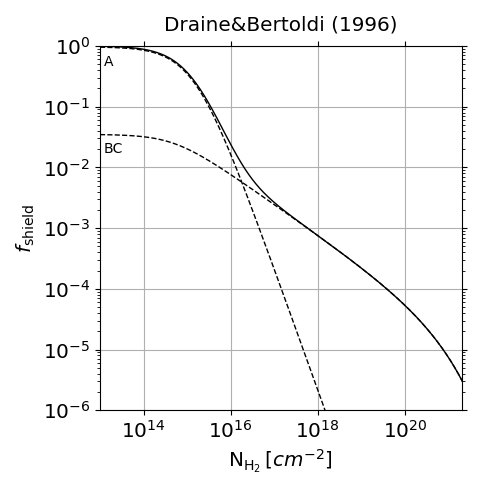
\includegraphics[width = 0.4\textwidth]{figure/H2/pomp/fshield.png}
    \caption{Fonction de shielding $f_\mathrm{shield}$ de $\mathrm{H}_2$ en fonction de la colonne densité $N(\mathrm{H}_2)$}
    \label{fig:H2:fshield}
\end{figure}


\subsubsection{Extinction par les grains}

Le champs de rayonnement calculé par le code ne prend pas en compte l'extinction par les grains. Approximation FGK. Je corrige le champs de rayonnement par $e^{-\tau_d}$ où $\tau_d = N_\mathrm{H}\sigma_d$ donné par \cite{SternbergLePetit2014} Eq 20. Ainsi, 

$$\chi^{'} = e^{-\tau_d
}\, f_{\mathrm{shield}}\, \chi$$


\subsection{Comparaison avec le code PDR de Meudon}

On récupère du code le taux de refroidissement $\Lambda_{\mathrm{PDR}}$ par la molécule $\mathrm{H}_2$ qui peut être positif ou négatif. Le taux prend en compte du chauffage par desexcitation collisionnelle et du refroidissement ro-vibrationelle (émission). Il ne prend pas en compte de la photodissociation (qui chauffe). On veut étudier le chauffage, on appelle $\Gamma_{\mathrm{PDR}}$ la partie négative du taux ($\Lambda_{\mathrm{PDR}} < 0$) et on le compare aux de chauffage nets.

\begin{equation}
    \begin{split}
        \Gamma_{\mathrm{Rollig} \, \mathrm{net}} &= \Gamma_{\mathrm{H}_2^\star} + \Lambda_{\mathrm{H}_2} \\ 
        \Gamma_{\mathrm{BS} \, \mathrm{net}} &=\Gamma_{\mathrm{H}_2 \, \mathrm{pump}} +  \Gamma_{\mathrm{H}_2 \, \mathrm{pd}} 
    \end{split}
\end{equation}

La figure \ref{fig:H2:GammaPDR} compare les taux de chauffages nets utilisant différentes prescriptions à celui calculé dans le code (en noir). Le chauffage calculé par Rollïg et de Bialy&Sternberg ont la même intensité en bord de nuage où la désexcitation collisionnelle est prédominante. 

L'approximation FGK est une méthode qui calcule le spectre du champs de rayonnements à travers le nuage qui prend en compte l'absorption dans le continuum et le carbone. Il prend également en compte l'écrantage de la molécule $\mathrm{H}_2$ (figure \ref{fig:H2:fgk} \cite{FGK}). 

\begin{figure}[h!]
    \centering
    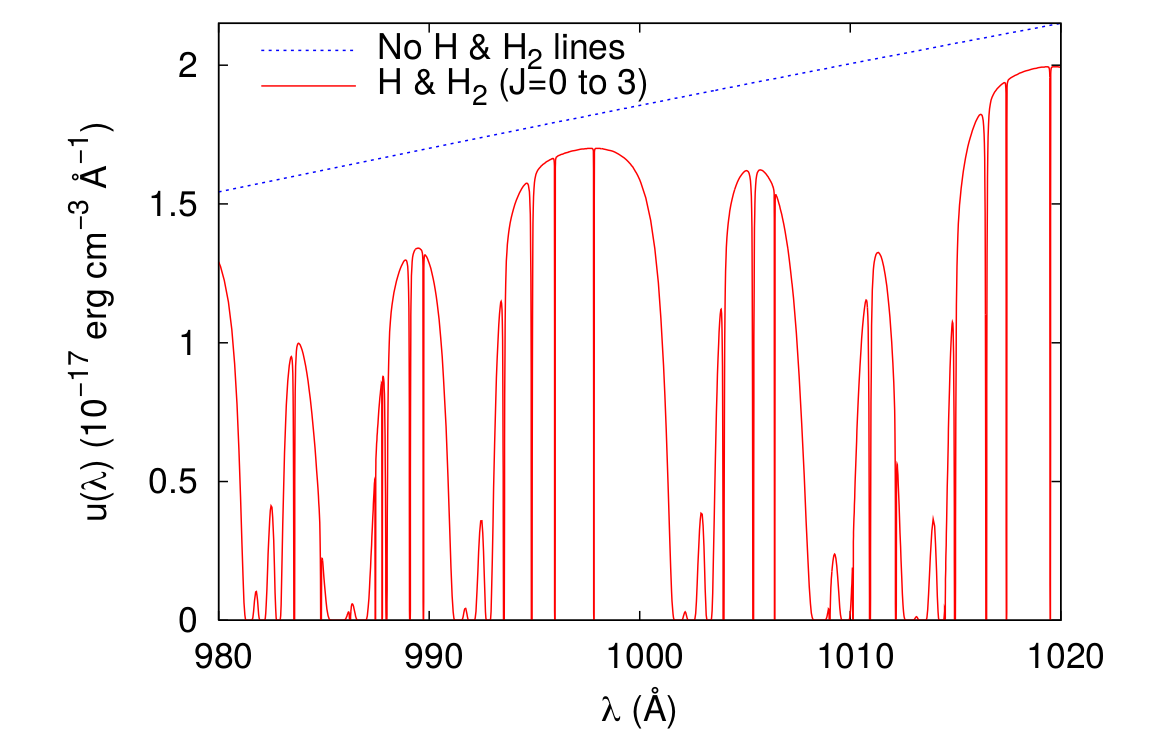
\includegraphics[width = 0.8\textwidth]{figure/H2/fgk.png}
    \caption{Densité d'énergie au sein d'un nuage à un $A_\mathrm{V}=0.5$. Les niveaux du $\mathrm{H}$ et de $\mathrm{H}_2$ absorbent certains photons sur certaines raies. A mesure que l'on s'enfonce dans le nuage beaucoup de matière se trouve sur la ligne de visée et les raies d'absroptions s'élargissent (voir optiquement épaisse Draine) \cite{FGK}}
    \label{fig:H2:fgk}
\end{figure}


\subsection{Prescription de Glover et Janev}

Dans la version \uncinq les taux de dissociation collisionelle de $\mathrm{H}_2$ via 

\begin{equation}
    \begin{array}{lcccccccl}
        \mathrm{H} & + & \mathrm{H}_2   & \rightarrow &\mathrm{H}  & + & \mathrm{H} & + & \mathrm{H} \\
        \mathrm{H}_2  & + & \mathrm{H}_2  & \rightarrow & \mathrm{H} & + &\mathrm{H}_2  & + & \mathrm{H} \\
    \end{array}
\end{equation}

sont calculé selon Janev (2008). Le passage à la nouvelle version du code (\unsept) qui utilise aussi la prescription de Janev ne change rien (encore heureux). Les raies du $\mathrm{H}_2$ et du $\mathrm{CO}$ sont les mêmes et le profils de température aussi. On utilise dorénavant pour cette étude la version \unsept. On compare maintenant la prescription de Glover à celle de Janev. \newline

%%%%%%%%%%%%%%%%%%%%%%%%%%%%%%%%%%%%%%%%%%%%%%%%%%%%%%%%%%%%%%%%%%%%%%%%%%%%%ùùùùù

\subsubsection{Bord Atomique - Janev/Glover}

Les grilles sont à compléter notamment H2noBossion. En bord de région atomique, le chauffage par $\mathrm{H}_2$ prédomine sur les mêmes types de PDR (figure \ref{fig:H2:JanevGlover:Gmax}). Les agents refroidissants sont différents (figure \ref{fig:H2:JanevGlover:Lmax}): les réactions chimiques cessent de devenir majoritaire avec la prescription de Glover. En effet la dissociation collisionelle de $\mathrm{H}_2$ qui est endothermique n'est plus favorisé avec la nouvelle prescription. Il fait également plus chaud en bord de nuage (montrer des profils).

\begin{figure}[!htbp]
    \centering
    \begin{subfigure}[t]{0.45\textwidth} % "0.45" donne ici la largeur de l'image
        \centering 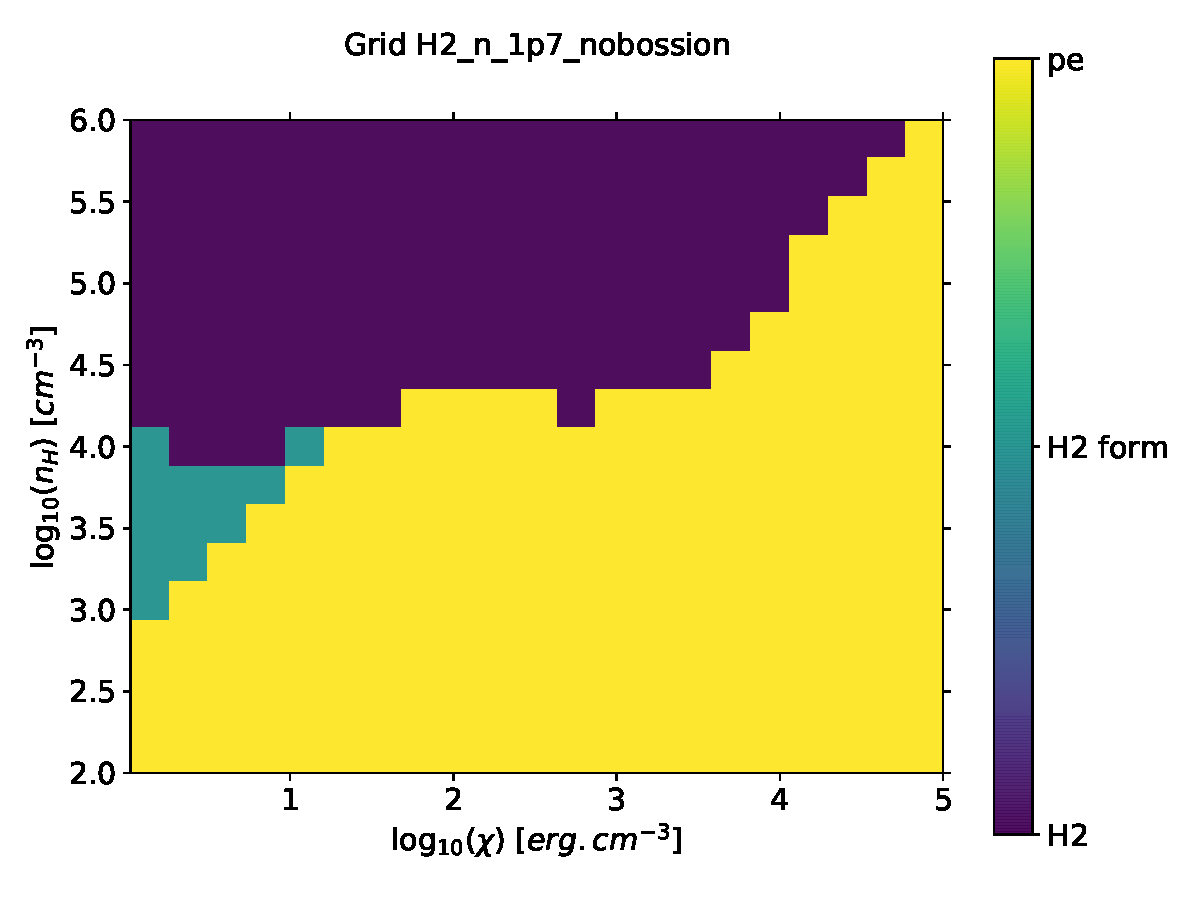
\includegraphics[trim = {0 0 0 0 },clip,width=1\textwidth]{figure/H2/JanevGlover/janev/mapGmax.pdf}
        \caption{Chauffage - Janev}
    \end{subfigure}
    ~ 
    \begin{subfigure}[t]{0.45\textwidth}
        \centering 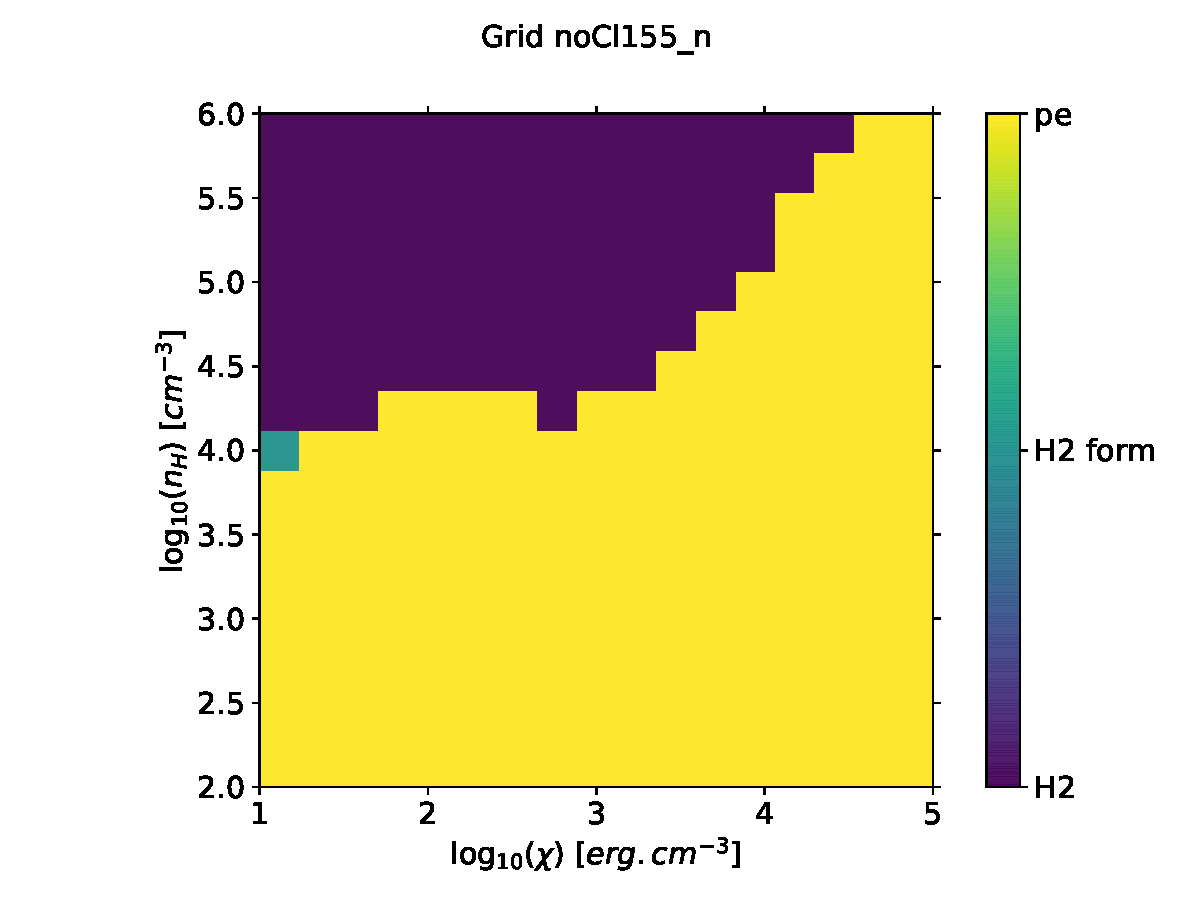
\includegraphics[trim = {0 0 0 0 },clip,width=1\textwidth]{figure/H2/JanevGlover/glover/mapGmax.pdf}
        \caption{Chauffage - Glover}
    \end{subfigure}
    \label{fig:H2:JanevGlover:Gmax}
    \caption{Taux de chauffage maximal en bord de région atomique}
    
    \begin{subfigure}[t]{0.45\textwidth} % "0.45" donne ici la largeur de l'image
        \centering 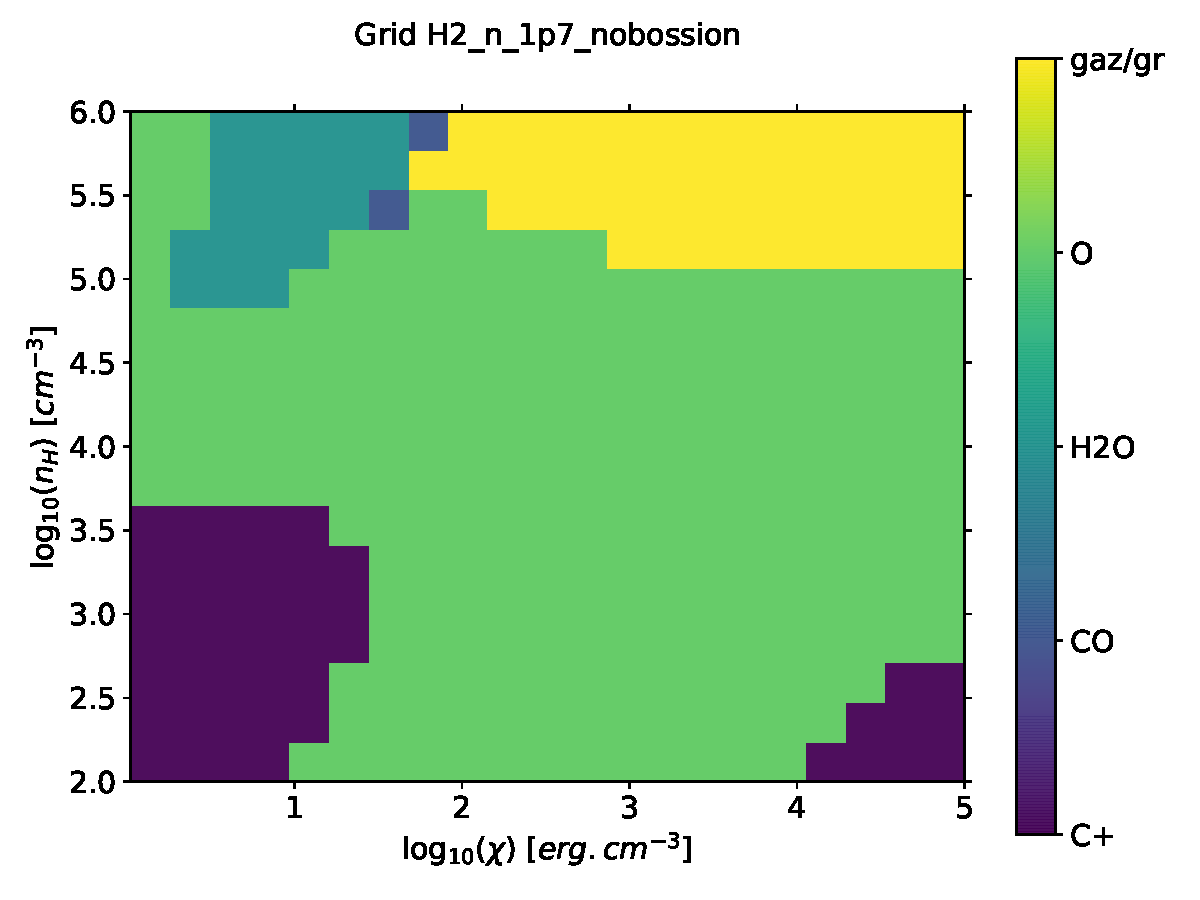
\includegraphics[trim = {0 0 0 0 },clip,width=1\textwidth]{figure/H2/JanevGlover/janev/mapLmax.pdf}
        \caption{Refroidissement - Janev}
    \end{subfigure}
    ~ 
    \begin{subfigure}[t]{0.45\textwidth}
        \centering 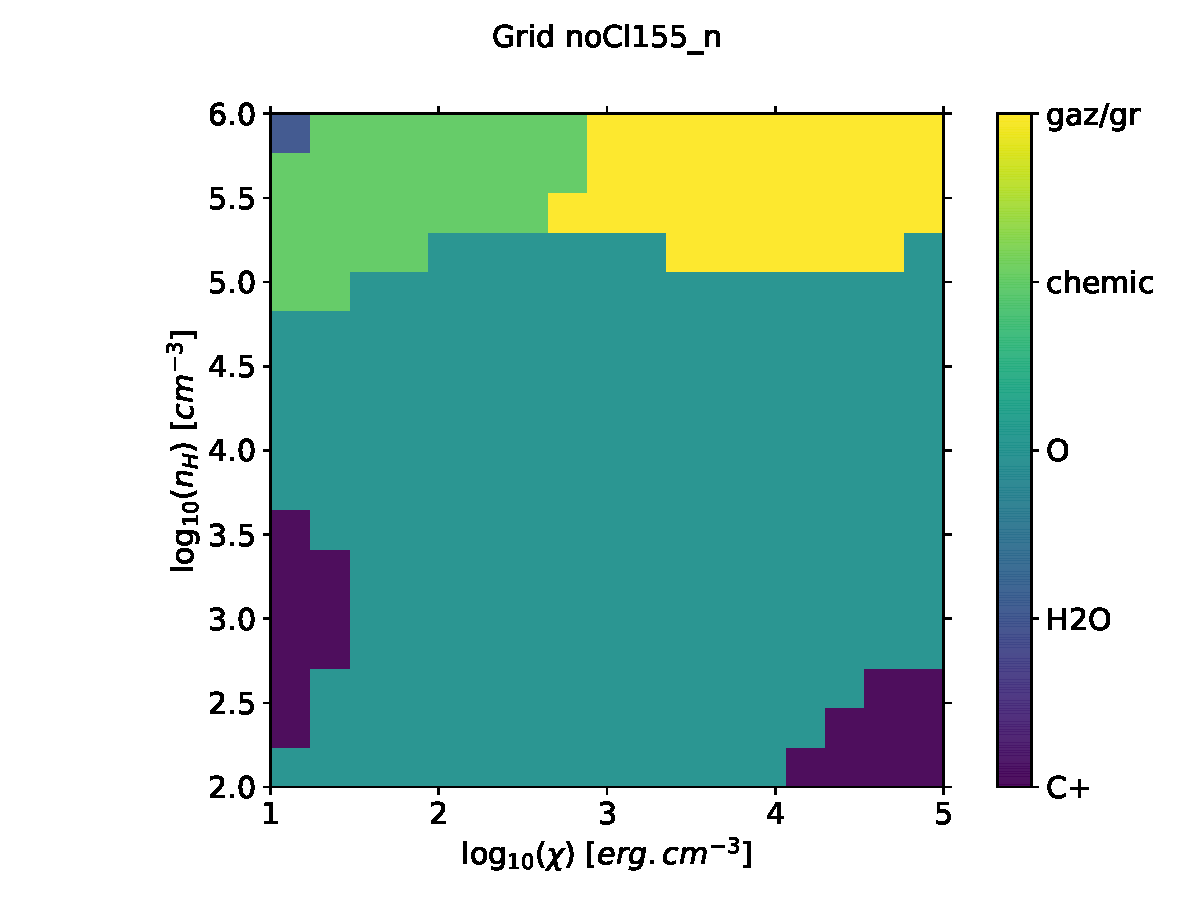
\includegraphics[trim = {0 0 0 0 },clip,width=1\textwidth]{figure/H2/JanevGlover/glover/mapLmax.pdf}
        \caption{Refroidissement - Glover}
    \end{subfigure}
    \caption{Taux de refroidissement maximal en bord de région atomique}
    
    \label{fig:H2:JanevGlover:Lmax}
\end{figure}

Le rapport $\Gamma_{\mathrm{H}_2}/\Gamma_{\mathrm{tot}}$, montre une légère diminution de l'efficacité du chauffage avec la prescription de Glover.  Mais dans les formules du chauffage par pompage de H2, augmenter un peu la température améliore le chauffage (il y a plus de collision), mais est ce que cela touche le taux de H2 en bord de nuage ? 

\textit{Est que le chauffage $\Gamma_\mathrm{H}_2$ perd de son efficacité en raison du chauffage un peu plus important ?}

\begin{figure}[!htbp]
    \centering
    \begin{subfigure}[t]{0.45\textwidth} % "0.45" donne ici la largeur de l'image
        \centering 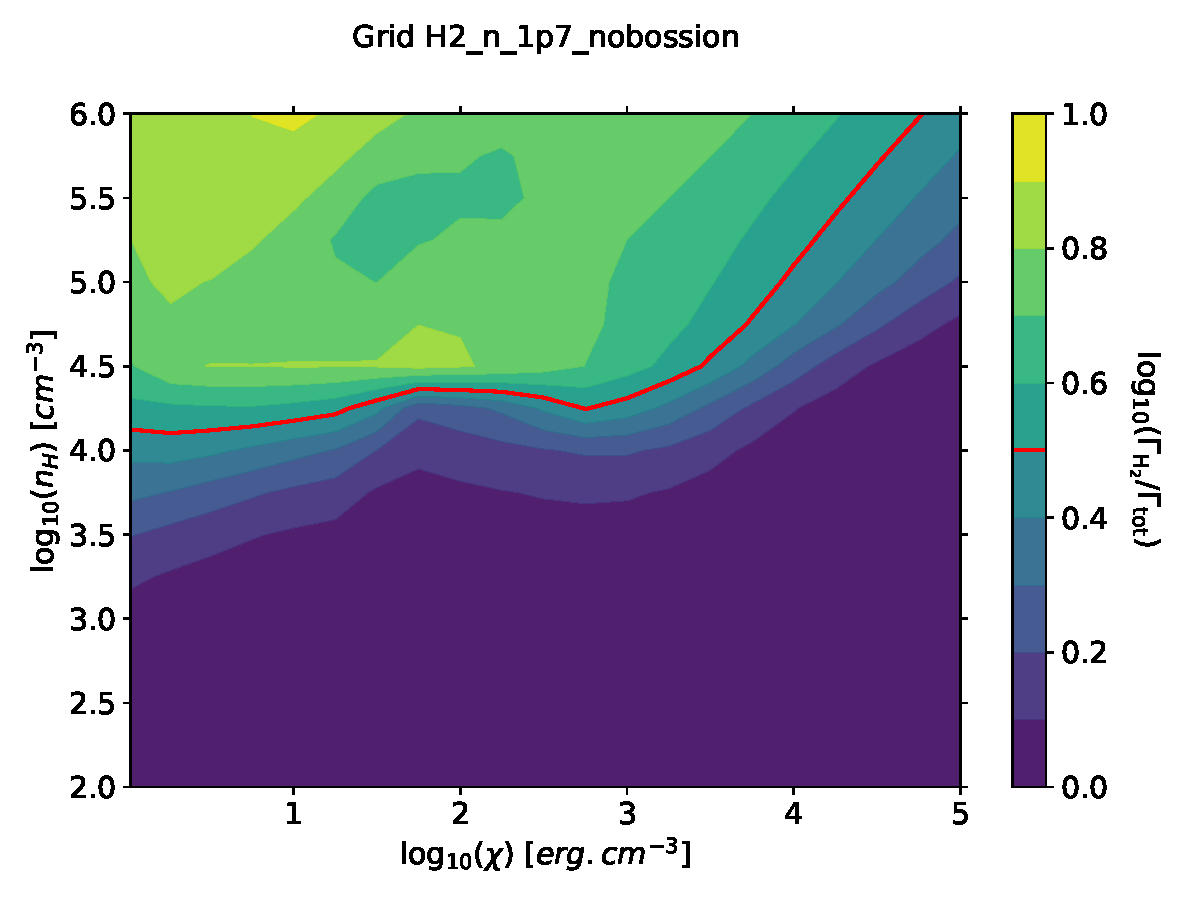
\includegraphics[trim = {0 0 0 0 },clip,width=1\textwidth]{figure/H2/JanevGlover/janev/mapG_H2.pdf}
        \caption{Janev}
    \end{subfigure}
    ~ 
    \begin{subfigure}[t]{0.45\textwidth}
        \centering 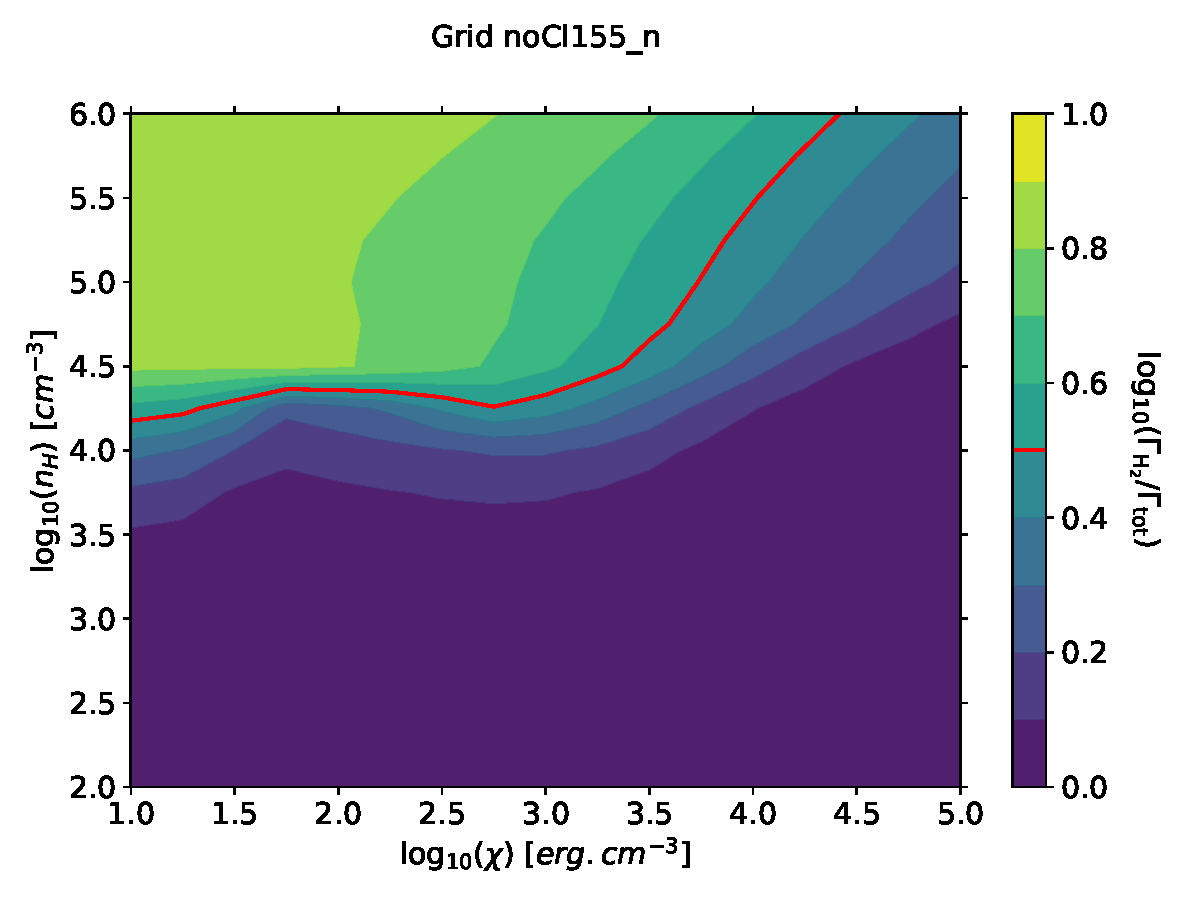
\includegraphics[trim = {0 0 0 0 },clip,width=1\textwidth]{figure/H2/JanevGlover/glover/mapG_H2.pdf}
        \caption{Glover}
    \end{subfigure}
    \caption{Taux de chauffage maximal en bord de région atomique}
    \label{fig:H2:JanevGlover:Gmax}
\end{figure}

%%%%%%%%%%%%%%%%%%%%%%%%%%%%%%%%%%%%%%%%%%%%%%%%%%%%%%%%%%%%%%%%%%%%%%%%%%%%%ùùùùù


\subsubsection{Transition $\mathrm{H}/\mathrm{H}_2$ - Janev/Glover}

Grâce à la formule de Glover on dépasse le plateau de $600 K$ qu'avait Franck. On atteint des températures allant jusqu'au millier de Kelvin (figure \ref{fig:H2:JanevGlover:THH2}). il faut refaire les carte. Pourquoi ? Il faudrait tracer les .res pour comparer les taux de chauffages et refroidissements aux points de la transition HH2. 

\begin{figure}[!htbp]
    \centering
    \begin{subfigure}[t]{0.45\textwidth} % "0.45" donne ici la largeur de l'image
        \centering 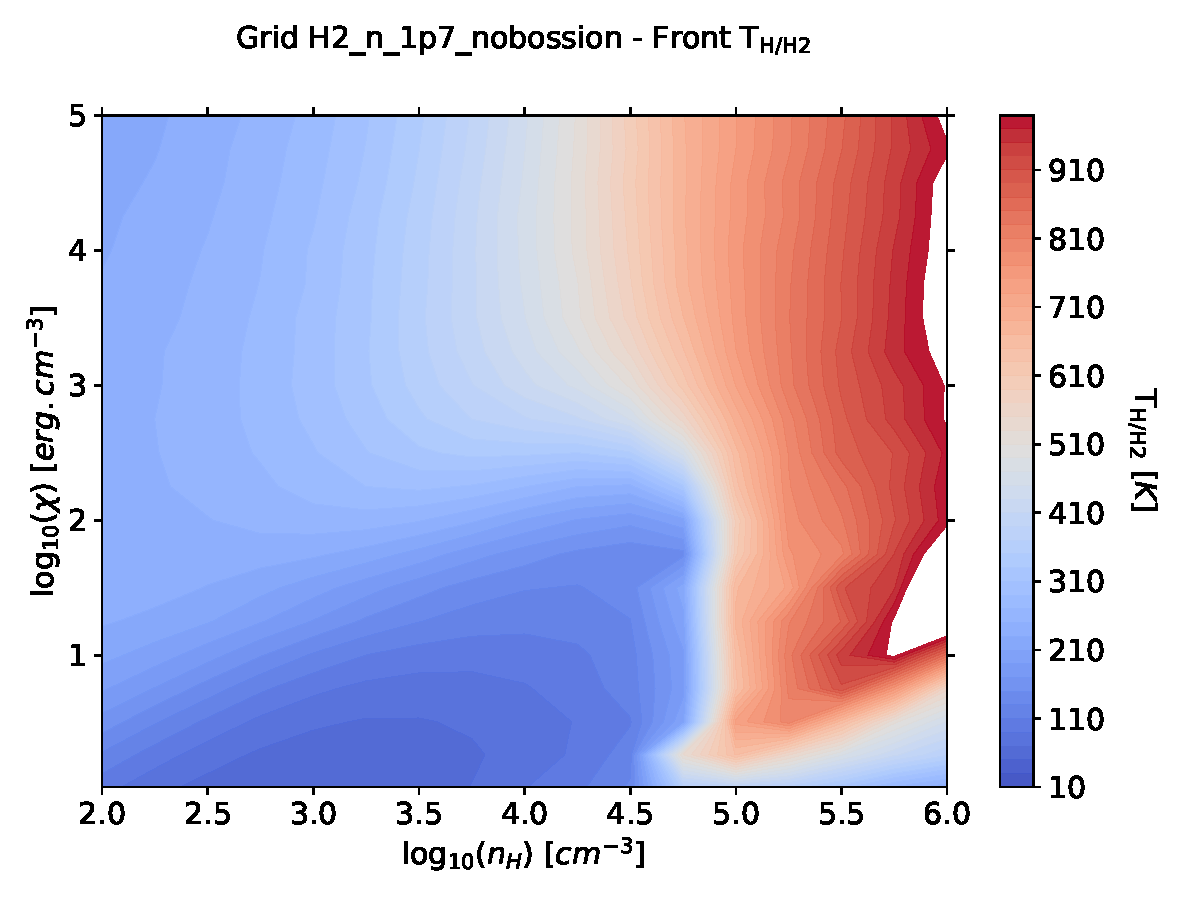
\includegraphics[trim = {0 0 0 0 },clip,width=1\textwidth]{figure/H2/JanevGlover/janev/HH2_T_Franck.pdf}
        \caption{Janev}
    \end{subfigure}
    ~ 
    \begin{subfigure}[t]{0.45\textwidth}
        \centering 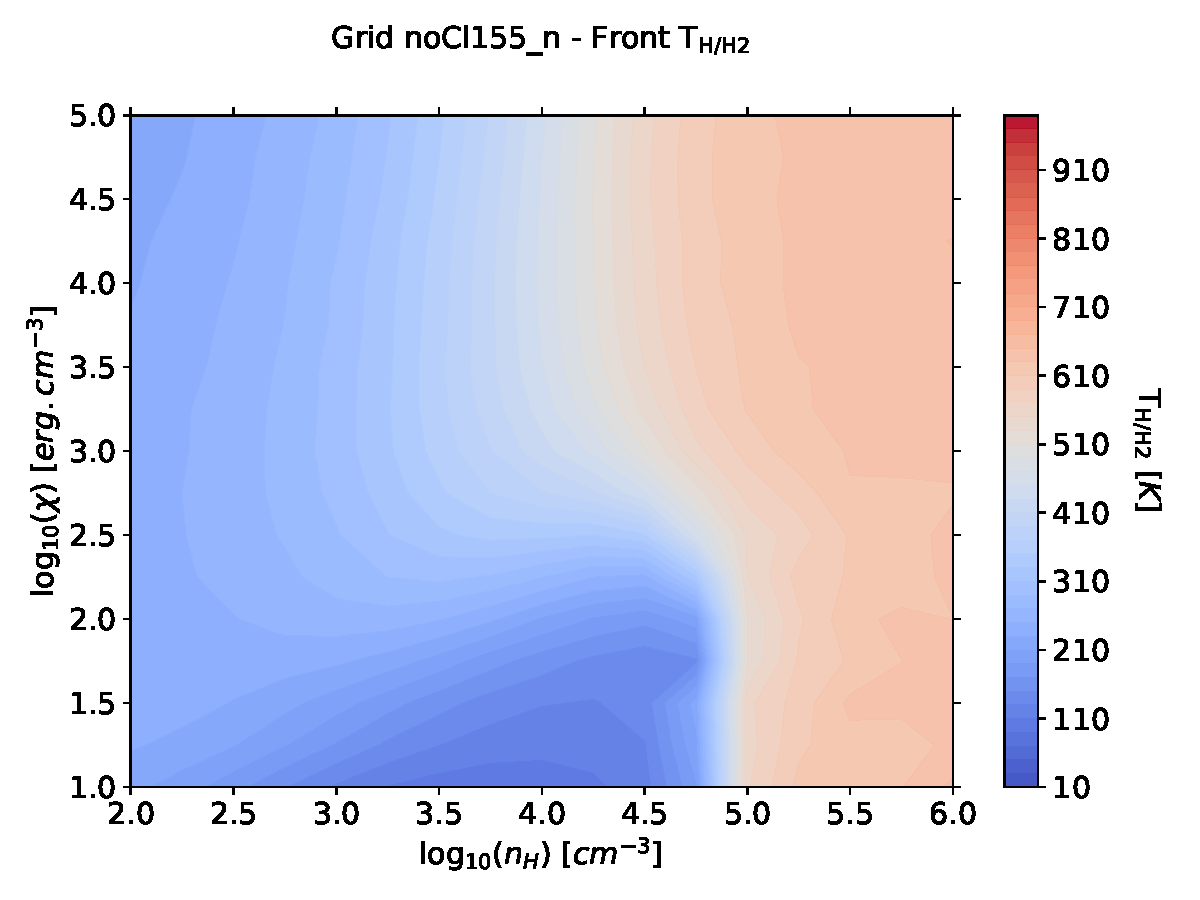
\includegraphics[trim = {0 0 0 0 },clip,width=1\textwidth]{figure/H2/JanevGlover/glover/HH2_T_Franck.pdf}
        \caption{Glover}
    \end{subfigure}
    \caption{Température transition HH2}
    \label{fig:H2:JanevGlover:THH2}
\end{figure}

Est ce que la région atomique augmente ? Franck aimerait car les observations ne sont pas très en accord avec les données observationelles. Sur la figure \ref{fig:H2:JanevGlover:AVHH2} on voit que la transition ne bouge pas tellement.

\begin{figure}[!htbp]
    \centering
    \begin{subfigure}[t]{0.45\textwidth} % "0.45" donne ici la largeur de l'image
        \centering 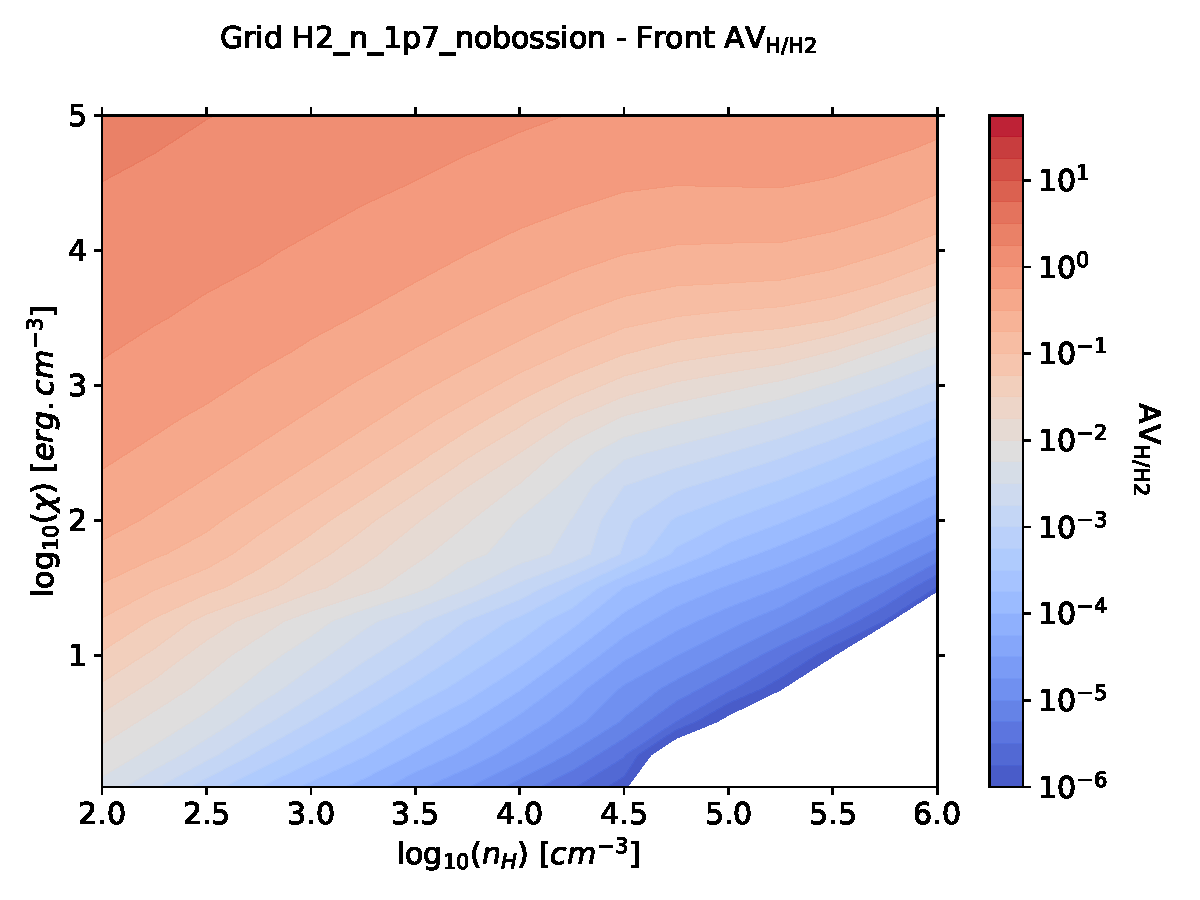
\includegraphics[trim = {0 0 0 0 },clip,width=1\textwidth]{figure/H2/JanevGlover/janev/HH2_AV_Franck.pdf}
        \caption{Janev}
    \end{subfigure}
    ~ 
    \begin{subfigure}[t]{0.45\textwidth}
        \centering 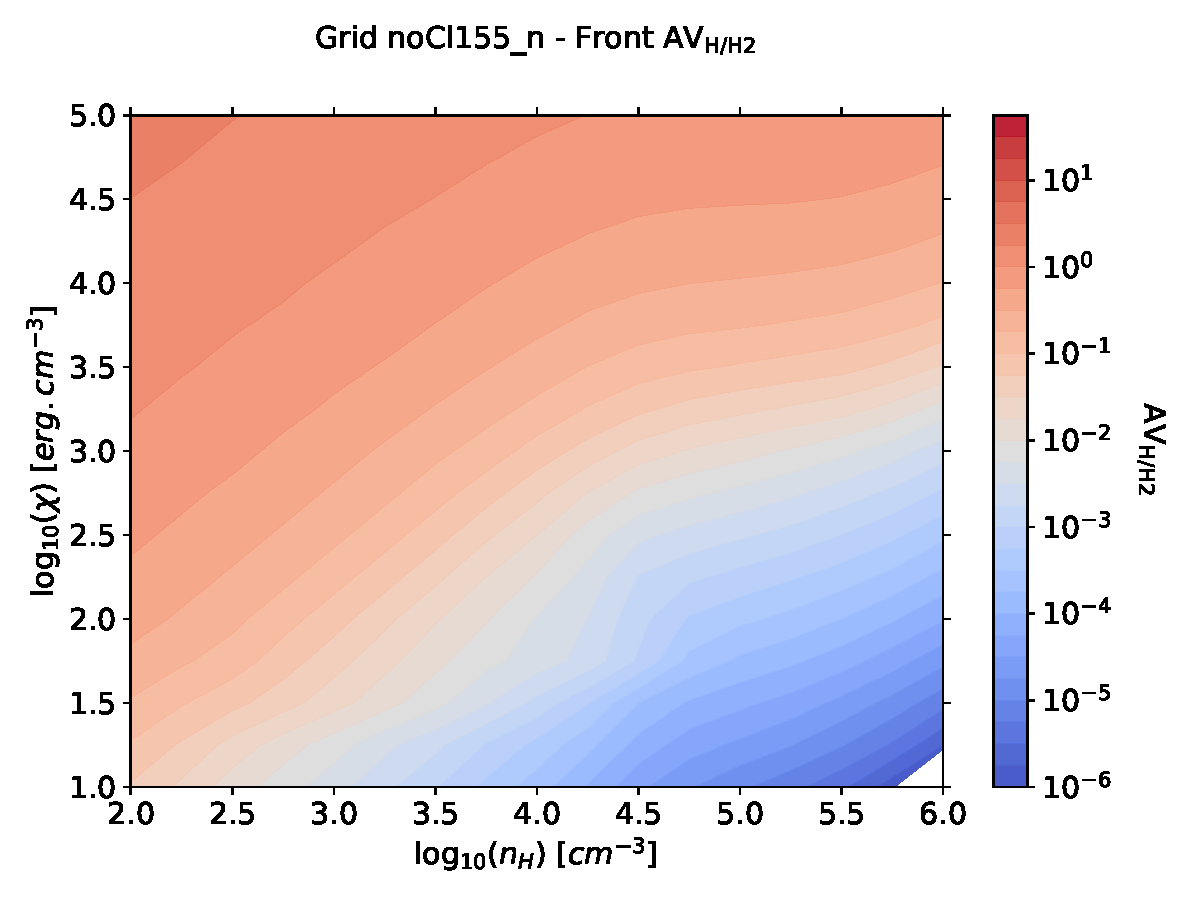
\includegraphics[trim = {0 0 0 0 },clip,width=1\textwidth]{figure/H2/JanevGlover/glover/HH2_AV_Franck.pdf}
        \caption{Glover}
    \end{subfigure}
    \caption{Température transition HH2}
    \label{fig:H2:JanevGlover:AVHH2}
\end{figure}

%%%%%%%%%%%%%%%%%%%%%%%%%%%%%%%%%%%%%%%%%%%%%%%%%%%%%%%%%%%%%%%%%%%%%%%%%%%%%ùùùùù


\subsubsection{Raies du $\mathrm{CO}$ et $\mathrm{H}_2$ - Janev/Glover}
à tracer en plus des profils de températures de modèles ...

% et on remarque plusieurs choses. Tout d'abord les raies d'émissions de $\mathrm{H}_2$ et $\mathrm{CO}$ sont augmentées (\autoref{figu:H2:..}). De plus le profil de température avec la nouvelle prescription (Glover) est modifié un tout petit peu au au bord (+100K) et un peu à l'entrée du nuage moléculaire (+400K) (\autoref{fig:H2:JanevGlover:emiss}). L'augmentation de la température à l'entrée du nuage moléculaire ($A_\mathrm{V} = 0.8$) provient du chauffage par exothermicité des réactions chimiques qui devient majeure (jusqu'à $50\%$ du chauffage total). Janev a tendance à surestimer les taux de dissociation qui sont toutes deux des réactions endothermiques et qui ont des efficacités de refroidissement les plus importantes. Les taux calculé par Glover réduisent leur refroidissement globale sur le nuage ce qui le chauffe. \newline 


% \begin{figure}[h!]
%     \centering
%     \begin{subfigure}[t]{0.45\textwidth} % "0.45" donne ici la largeur de l'image
%         \centering 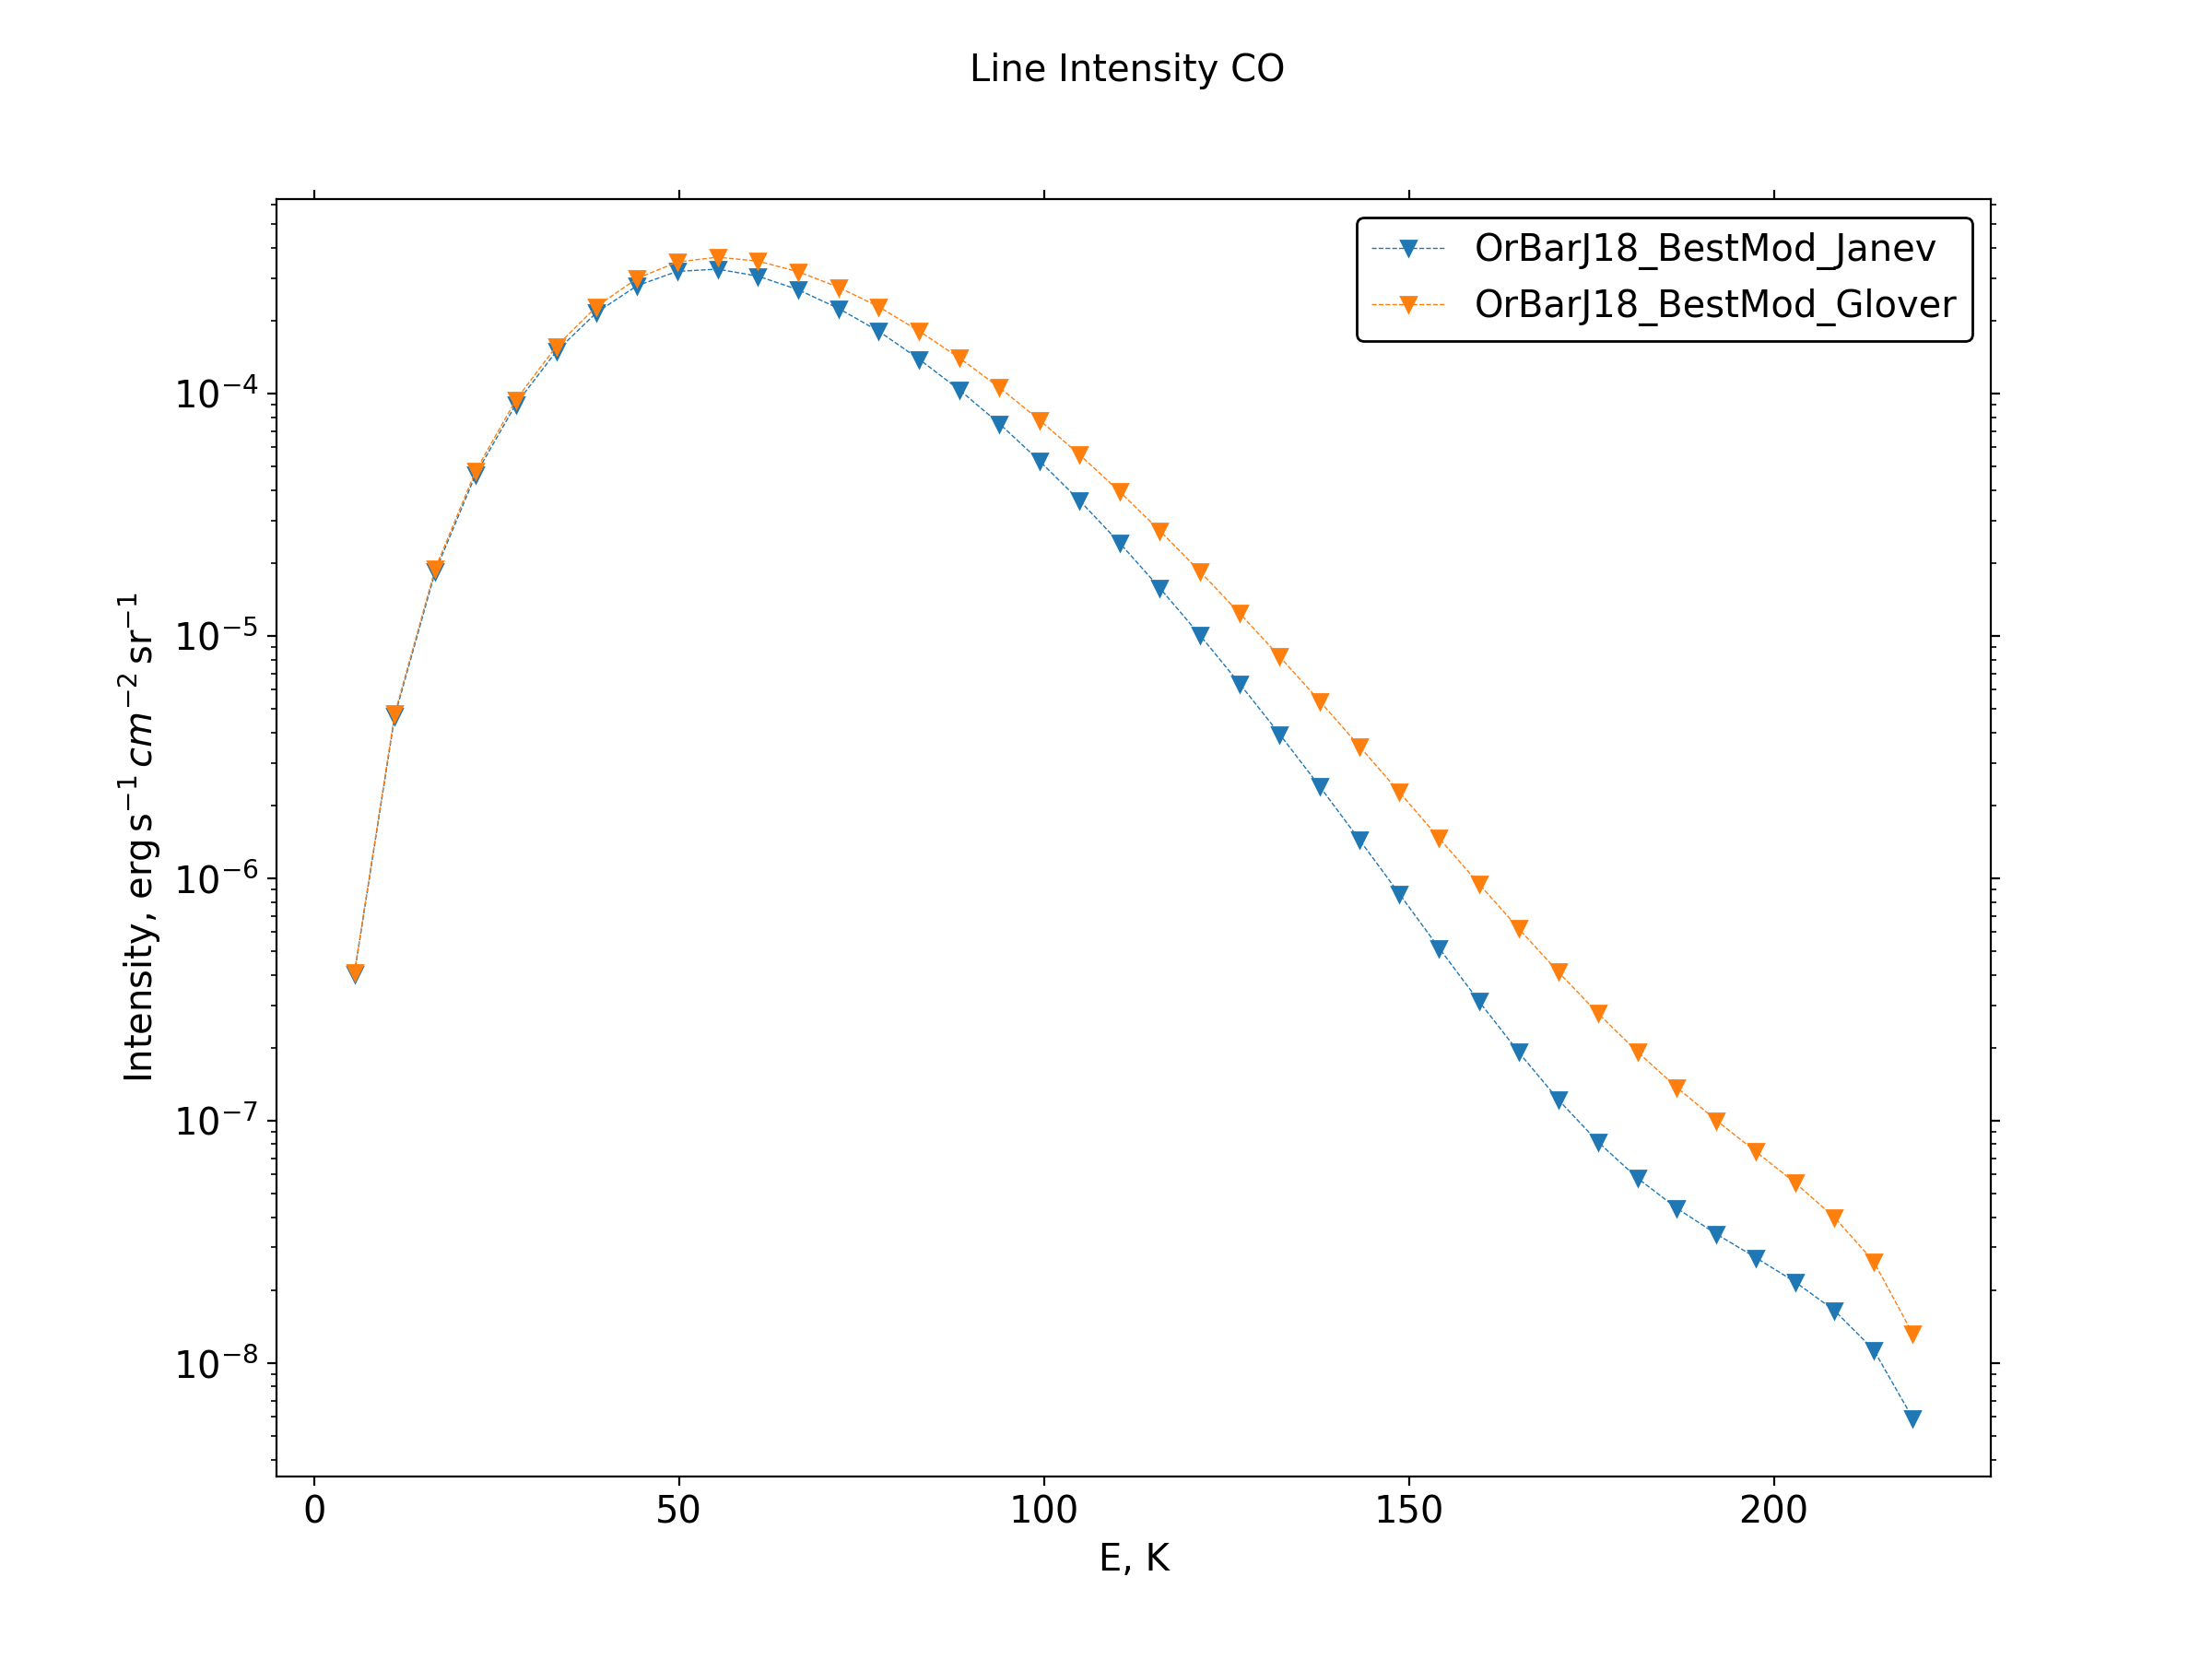
\includegraphics[trim = {0 0 0 1.5cm},clip,width=1\textwidth]{figure/H2/JanevGlover/I_comp_CO.png}
%         \caption{Spectre $\mathrm{H}_2$}
%     \end{subfigure}
%     ~ 
%     \begin{subfigure}[t]{0.45\textwidth}
%         \centering \includegraphics[trim = {0 0 0 1.5cm},clip,width=1\textwidth]{figure/H2/JanevGlover/nT_comp_CO.png}
%         \caption{Profil de densité et température de $\mathrm{H}_2$}
%     \end{subfigure}

%     \centering
%     \begin{subfigure}[t]{0.45\textwidth} % "0.45" donne ici la largeur de l'image
%         \centering \includegraphics[trim = {0 0 0 1.5cm},clip,width=1\textwidth]{figure/H2/JanevGlover/I_comp_H2.png}
%         \caption{Spectre de $\mathrm{CO}$}
%     \end{subfigure}
%     ~ 
%     \begin{subfigure}[t]{0.45\textwidth}
%         \centering \includegraphics[trim = {0 0 0 1.5cm},clip,width=1\textwidth]{figure/H2/JanevGlover/nT_comp_H2.png}
%         \caption{Profil de densité et température de $\mathrm{CO}$}
%     \end{subfigure}
%     \caption{Impact des prescriptions de Janev et Glover sur les raies d'émissions des traceurs $\mathrm{H}_2$ et $\mathrm{CO}$}
%     \label{fig:H2:JanevGlover:emiss}
% \end{figure}


% Néanmoins on connaît mal la proportion effective qui chauffe le gaz par exothermicité. Il faut reprendre l'étude sur l'exothermicité des réactions chimiques en jouant sur la prescription. \newline 

% On cherche à visualiser l'impact des nouveaux calculs des niveaux de $\mathrm{H}_2$ sur les raies. On l'a calculé dans le cas de Janev et Glover mais l'on montre seulement la prescription de Glover qui est la plus importante (\autoref{fig:H2:GloverBossion:emiss})

% On se rend compte que l'impact est minime alors que le travail pour calculer ces niveaux est lourd. Au moins on sait que connaître précisément les niveaux de $\mathrm{H}_2$ n'est pas décisif dans l'interprétation des spectres d'émissions. 

% \begin{figure}[h!]
%     \centering
%     \begin{subfigure}[t]{0.45\textwidth} % "0.45" donne ici la largeur de l'image
%         \centering \includegraphics[trim = {0 0 0 1.5cm},clip,width=1\textwidth]{figure/H2/GloverBossion/I_comp_CO.png}
%         \caption{Spectre $\mathrm{H}_2$}
%     \end{subfigure}
%     ~ 
%     \begin{subfigure}[t]{0.45\textwidth}
%         \centering \includegraphics[trim = {0 0 0 1.5cm},clip,width=1\textwidth]{figure/H2/GloverBossion/nT_comp_CO.png}
%         \caption{Profil de densité et température de $\mathrm{H}_2$}
%     \end{subfigure}

%     \centering
%     \begin{subfigure}[t]{0.45\textwidth} % "0.45" donne ici la largeur de l'image
%         \centering \includegraphics[trim = {0 0 0 1.5cm},clip,width=1\textwidth]{figure/H2/GloverBossion/I_comp_H2.png}
%         \caption{Spectre de $\mathrm{CO}$}
%     \end{subfigure}
%     ~ 
%     \begin{subfigure}[t]{0.45\textwidth}
%         \centering \includegraphics[trim = {0 0 0 1.5cm},clip,width=1\textwidth]{figure/H2/GloverBossion/nT_comp_H2.png}
%         \caption{Profil de densité et température de $\mathrm{CO}$}
%     \end{subfigure}
%     \caption{Comparaison des raies d'émissions des traceurs $\mathrm{H}_2$ et $\mathrm{CO}$ entre les calculs avec ou sans Bossion}
%     \label{fig:H2:GloverBossion:emiss}
% \end{figure}


\subsection{Où le chauffage par $\mathrm{H}_2$ prédomine-t-il dans le nuage ?}

On trace sur la figure ... le type de chauffage prédominant en bord de nuage. En comparant à la version \uncinq, sans le chlore (Janev) on se rend compte que la zone concerné par le chauffage par $\mathrm{H}_2$ est plus large et joue pour des région à plus fort champs de rayonnement. \newline

\begin{figure}[h!]
    \centering
    \includegraphics[width = 0.6\textwidth]{figure/H2/mapGloverBossion/mapGmax.png}
    \caption{}
    \label{fig:H2:mapGloverBossion:Gmax}
\end{figure}

On trace le profil de température de quelques modèles (\autoref{fig:H2:mapGloverBossion:profilTx}). 
\begin{itemize}
    \item On voit (d) que la température au bord du nuage augmente pour les fort champs de rayonnement et que cette tendance est moins vraie (c) si le chauffage par $\mathrm{H}_2$ cesse de prédominer en bord de nuage. Il vient un $\chi$ où la température augmente de manière raide à l'entrée du nuage moléculaire (a). Je présume que c'est la recombinaison sur les grains qui est accéléré par le début de formation de $\mathrm{H}_2$ mais A VERIFIER. Comparer les $\Gamma$ et $\Lambda$ en fonction de la profondeur du nuage pour quelques modèles qui nous intéresse.
    \item Si l'on s'enfonce en $\chi$ (b) le chauffage par $\mathrm{H}_2$ commence à prédominer en bord de nuage et on voit qu'il efface l'augmentation de température en bord de nuage moléculaire. Cela se voit aussi en comarant (a) et (c).
    \item A forte densité (d) il apparaît un plateau après la transition $\mathrm{H}/\mathrm{H}_2$ : est ce que cela est du à l'effet photoélectrique ? pourrait il exciter d'avantage les raies du H2 ? On a vu avant qu'elle pouvait être du au chauffage par réactions chimiques qui devenait important car Glover tue la dissociation du H2. Et si l'on tracait ce T à cet endroit du nuage dans l'espace des paramètres. Peut être que l'on verrait aussi un bistabilité ? (première fois ou le gradient de T est minimale après la transition)
    \item La température de la transition ne change pas d'un poil avec $\chi$ mais bouge avec la densité. Un fort champ de rayonnement ne fera que déplacer l'AV mais pas la température. Se comprend un peu car $\Gamma \propto n^2$ et $\Lambda \propto n $ mais pas toujours $\propto \chi$.
\end{itemize}

\begin{figure}[h!]
    \centering
    \begin{subfigure}[t]{0.45\textwidth} % "0.45" donne ici la largeur de l'image
        \centering \includegraphics[trim = {0 0 0 0},clip,width=1\textwidth]{figure/H2/mapGloverBossion/H2_n_1p7_bossion_d3p5r2p5_d3p5r3p5_d3p5r4p5.png} 
        \caption{}
    \end{subfigure}
    ~ 
    \begin{subfigure}[t]{0.45\textwidth}
        \centering \includegraphics[trim = {0 0 0 0},clip,width=1\textwidth]{figure/H2/mapGloverBossion/H2_n_1p7_bossion_d3p5r4p5_d4p5r4p5_d5p5r4p5.png}
        \caption{}
    \end{subfigure}

    \centering
    \begin{subfigure}[t]{0.45\textwidth} % "0.45" donne ici la largeur de l'image
        \centering \includegraphics[trim = {0 0 0 0},clip,width=1\textwidth]{figure/H2/mapGloverBossion/H2_n_1p7_bossion_d4p5r2p5_d4p5r3p5_d4p5r4p5.png} 
        \caption{}
    \end{subfigure}
    ~ 
    \begin{subfigure}[t]{0.45\textwidth}
        \centering \includegraphics[trim = {0 0 0 0},clip,width=1\textwidth]{figure/H2/mapGloverBossion/H2_n_1p7_bossion_d5p5r2p5_d5p5r3p5_d5p5r4p5.png} 
        \caption{}
    \end{subfigure}
    \caption{Profil de températures pour différent modèles de la grille (Glover + Bossion). La croix indique la température de la transition $\mathrm{H}/\mathrm{H}_2$ : $n(\mathrm{H})=2n(\mathrm{H}_2)$.}
    \label{fig:H2:mapGloverBossion:profilTx}
\end{figure}

\subsection{Dans quelles conditions le chauffage par $\mathrm{H}_2$ prédomine-t-il ?}

On observe également la température de la transition $\mathrm{H}/\mathrm{H}_2$ dans l'espace des paramètres (\autoref{fig:H2:mapGloverBossion:mapTHH2}). La température ne dépend toujours pas de l'intensité du champs de rayonnements. On voit que l'on arrive à dépasser le plateau des (600K) que Franck avait avec Janev. La dissociation étant moins importante on peut avoir du gaz plus chaud. Il sera plus facile de comprendre si c'est uniquement grâce à Bossion ou Glover. \newline 

\begin{figure}[th!]
    \centering
    \begin{subfigure}[t]{0.45\textwidth} % "0.45" donne ici la largeur de l'image
        \centering \includegraphics[trim = {0 0 0 0},clip,width=1\textwidth]{figure/H2/mapGlovernoBossion/HH2_T_Franck.png}
        \caption{}
    \end{subfigure}
    ~ 
    \begin{subfigure}[t]{0.45\textwidth}
        \centering \includegraphics[trim = {0 0 0 0},clip,width=1\textwidth]{figure/H2/mapGloverBossion/HH2_T_Franck.png}
        \caption{}
    \end{subfigure}
    \caption{Carte de températures de la transition $\mathrm{H}/\mathrm{H}_2$ : $n(\mathrm{H})=2n(\mathrm{H}_2)$ avec ou sans les niveaux de Bossion (toujours Glover)}
    \label{fig:H2:mapGloverBossion:mapTHH2}
\end{figure}

\underline{Conclusion partielle :} il reste à s'assurer si la zone concernée est du à la nouvelle prescription de Glover ou aux calculs semi classique des niveaux de $\mathrm{H}_2$. Sinon, on voit que le chauffage par $\mathrm{H}_2$ concerne les régions denses et impactent principalement les bords atomiques. Or c'est si l'on chauffait l'entrée du nuage que l'on pourrait espérer observer les changements. Il faudrait regarder les diagrammes d'excitations de quelques espèces comme $\mathrm{H}_2$ ou $\mathrm{CO}$. On se pose également une question sur l'impact de la raideur de la transition sur la température (\autoref{fig:H2:mapGloverBossion:smooth}) : dans certains cas, la transition se fait pour des gaz encore chaud ce qui signifie que l'on pourrait voir des raies plus excitées. Dans quelles conditions ces phénomènes ont ils lieux ? Est ce que cela a un impact sur les raies ? (Sternberg 2014) Enfin on n'a pas observé les instabilités que pouvait provoquer le $\mathrm{H}_2$. Tracer quelques courbes de chauffages et refroidissements pour différent modèles (là le gradient de Tmax) est maximale par exemple. On observait également mieux l'instabilité sur des modèles isobares : faire une petite grille. Pour avancer sur cette histoire de chauffage par réaction chimiqie : tracer $\max_{AV} \Gamma_{ch}/\Gamma_{tot}$ dans l'espace des paramètres et le $(argmax_{AV}  \Gamma_{ch}/\Gamma_{tot})/AV_{HH2}$ qui est lié également au $\mathrm{H}_2$ par la réaction avec le $\mathrm{CH}^+$

\begin{figure}[th!]
        \centering \includegraphics[trim = {0 0 0 0},clip,width=0.5\textwidth]{figure/H2/mapGloverBossion/H2_n_1p7_bossion_d3p5r2p5_d4p5r2p5_d5p5r2p5.png}
        \caption{Profils de températures de différents modèles de la grille (Glover + Bossion)}
        \label{fig:H2:mapGloverBossion:smooth}
\end{figure}

\subsection{Dans quelles conditions peut on voir une instabilité ?}
\subsection{Quel est l'impact sur les raies des traceurs ?}



%%%%%%%%%%%%%%%%%%%%%%%%%%%%%%%%%%%%%%%%%%%%%%%%%%%%%%%%%%%%%%%%%%%%%%%%%%%%%%%%%%%%%%%%%%%%%%%%%%%%%%%%
\section*{Conclusion}


\clearpage
\bibliographystyle{apalike}
\bibliography{bib}

\clearpage
\begin{appendices}

%%%%%%%%%%%%%%%%%%%%%%%%%%%%%%%%%%%%%%%%%%%%%%%%%%%%%%%%%%%%%%%%%%%%%%%%%%%%



\section{Impact du chlore} 
\label{appendix:chlore}
\subsection*{Traceurs atomiques}
\begin{figure}[!h]
    \centering \includegraphics[trim = {0 0 0 1cm},clip,width=1\textwidth]{figure/Cl/gridModelEmiss/I_comp_Np.pdf}
        \caption{$\mathrm{N}^+$}
        \label{fig:cl:emiss:Np}
\end{figure}

\begin{figure}[!h]
    \centering \includegraphics[trim = {0 0 0 1cm},clip,width=1\textwidth]{figure/Cl/gridModelEmiss/I_comp_S.pdf}
        \caption{Diagramme d'intensité de $\mathrm{S}$}
        \label{fig:cl:emiss:S}
\end{figure}

\begin{figure}[!h]
    \centering \includegraphics[trim = {0 0 0 1cm},clip,width=1\textwidth]{figure/Cl/gridModelEmiss/I_comp_Si.pdf}
        \caption{Diagramme d'intensité de $\mathrm{Si}$}
        \label{fig:cl:emiss:Si}
\end{figure}

\begin{figure}[!h]
    \centering
    \begin{subfigure}[t]{0.49\textwidth} % "0.49" donne ici la largeur de l'image
        \centering \includegraphics[trim = {0 0 0 0},clip,width=1\textwidth]{figure/Cl/gridModelEmiss/nT_comp_Np.pdf}
        \caption{$\mathrm{N}^+$}
    \end{subfigure}
    ~ 
   \begin{subfigure}[t]{0.49\textwidth} % "0.49" donne ici la largeur de l'image
        \centering \includegraphics[trim = {0 0 0 0},clip,width=1\textwidth]{figure/Cl/gridModelEmiss/nT_comp_N.pdf}
        \caption{$\mathrm{N}$}
    \end{subfigure}
    
    \begin{subfigure}[t]{0.49\textwidth} % "0.49" donne ici la largeur de l'image
        \centering \includegraphics[trim = {0 0 0 0},clip,width=1\textwidth]{figure/Cl/gridModelEmiss/nT_comp_S.pdf}
        \caption{$\mathrm{S}$}
    \end{subfigure}
    ~
    \begin{subfigure}[t]{0.49\textwidth} % "0.49" donne ici la largeur de l'image
        \centering \includegraphics[trim = {0 0 0 0},clip,width=1\textwidth]{figure/Cl/gridModelEmiss/nT_comp_Si.pdf}
        \caption{$\mathrm{Si}$}
    \end{subfigure}
    
    \caption{Profils de densité des traceurs impactés par l'ajout du chlore.}
    \begin{minipage}{\textwidth}
    Il est représenté en trait plein les profils du modèle avec le chlore et en trait pointillé le modèle ne contenant pas de chlore. La température est en rouge et la densité en noir. On constate que l'augmentation de la température induit epar le chlore facilite la formation de ces traceurs. 
    \end{minipage}
    \label{fig:Cl:gridModelEmiss:nT:yes}
\end{figure}

\clearpage
\subsection*{Traceurs moléculaires}


\begin{figure}[!h]
        \centering \includegraphics[trim = {0 0 0 1cm},clip,width=1\textwidth]{figure/Cl/gridModelEmiss/I_comp_CS.pdf}
        \caption{Diagramme d'intensités du $\mathrm{CS}$}
        \label{fig:cl:emiss:CS}
\end{figure}

\begin{figure}[!h]
        \centering \includegraphics[trim = {0 0 0 1cm},clip,width=1\textwidth]{figure/Cl/gridModelEmiss/I_comp_H2O.pdf}
        \caption{Diagramme d'intensités du $\mathrm{H}_2\mathrm{O}$}
        \label{fig:cl:emiss:H2O}
\end{figure}

\begin{figure}[!h]
        \centering \includegraphics[trim = {0 0 0 1cm},clip,width=1\textwidth]{figure/Cl/gridModelEmiss/I_comp_H2.pdf}
        \caption{Diagramme d'intensités du $\mathrm{H}_2$}
        \label{fig:cl:emiss:H2}
\end{figure}

\begin{figure}[!h]
        \centering \includegraphics[trim = {0 0 0 1cm},clip,width=1\textwidth]{figure/Cl/gridModelEmiss/I_comp_CO.pdf}
        \caption{Diagramme d'intensités du $\mathrm{CO}$. Seules les transitions rotationnelles ont été écrites (toutes s'effectuent à $\mathrm{v}=0$)}
        \label{fig:cl:emiss:CO}
\end{figure}


\begin{figure}[!h]
    \centering
    \begin{subfigure}[t]{0.49\textwidth} % "0.49" donne ici la largeur de l'image
        \centering \includegraphics[trim = {0 0 0 0},clip,width=1\textwidth]{figure/Cl/gridModelEmiss/nT_comp_CS.pdf}
        \caption{$\mathrm{CS}$}
    \end{subfigure}
    ~ 
   \begin{subfigure}[t]{0.49\textwidth} % "0.49" donne ici la largeur de l'image
        \centering \includegraphics[trim = {0 0 0 0},clip,width=1\textwidth]{figure/Cl/gridModelEmiss/nT_comp_H2O.pdf}
        \caption{$\mathrm{H}_2\mathrm{O}$}
    \end{subfigure}
    
    \begin{subfigure}[t]{0.49\textwidth} % "0.49" donne ici la largeur de l'image
        \centering \includegraphics[trim = {0 0 0 0},clip,width=1\textwidth]{figure/Cl/gridModelEmiss/nT_comp_H2.pdf}
        \caption{$\mathrm{H}_2$}
    \end{subfigure}
    ~ 
    \begin{subfigure}[t]{0.49\textwidth} % "0.49" donne ici la largeur de l'image
        \centering \includegraphics[trim = {0 0 0 0},clip,width=1\textwidth]{figure/Cl/gridModelEmiss/nT_comp_CO.pdf}
        \caption{$\mathrm{CO}$}
    \end{subfigure}
    
    \caption{Profils de densité et de températures des traceurs impactés par l'ajout du chlore. Mêmes conventions que pour la figure \ref{fig:Cl:gridModelEmiss:nT:yes}. Les traceurs moléculaires sont peu modifiés par l'augmentation de la température de la zone atomique du nuage. }
    \label{fig:Cl:gridModelEmiss:nT:no}
\end{figure}


%%%%%%%%%%%%%%%%%%%%%%%%%%%%%%%%%%%%%%%%%%%%%%%%%%%%%%%%%%%%%%%%%%%%%%%%%%%%%%%%%%%%%%%%%%%%%
\clearpage
\section{Réactions chimiques initiées par $\mathrm{H}_2$}
\label{appendix:type46}
\begin{figure}[!h]
    \centering \includegraphics[trim = {0 0 0 1cm},clip,width=1\textwidth]{figure/type46/I_comp_H2.pdf}
    \caption{Diagramme d'intensité du $\mathrm{H}_2$}
    \begin{minipage}{\textwidth}
    
    \end{minipage}
    \label{fig:type46:H2}
\end{figure}

\begin{figure}[!h]
    \centering \includegraphics[trim = {0 0 0 1cm},clip,width=1\textwidth]{figure/type46/I_comp_H2O.pdf}
    \caption{Diagramme d'intensité du $\mathrm{H}_2\mathrm{O}$}
    \begin{minipage}{\textwidth}
  
    \end{minipage}
    \label{fig:type46:H2O}
\end{figure}

\begin{figure}[!h]
    \centering \includegraphics[trim = {3cm 3cm 3cm 7cm},clip,width=0.8\textwidth]{figure/type46/ChimieCO_1.pdf}
    \caption{Ancien réseau de formation du $\mathrm{CO}$}
    \label{fig:type46:form:COold}
\end{figure}


%%%%%%%%%%%%%%%%%%%%%%%%%%%%%%%%%%%%%%%%%%%%%%%%%%%%%%%%%%%%%%%%%%%%%%%%%
\clearpage
\section{Impact de la prescription de Glover}

% On a rassemblé dans cette section les figures servant à l'analyse mais qui sont trop volumineuse dans le rapport.

\vfill
\begin{figure}[!h]
    \centering
    \begin{subfigure}[t]{0.49\textwidth} % "0.49" donne ici la largeur de l'image
        \centering \includegraphics[trim = {0 0 0 0 },clip,width=1\textwidth]{figure/H2/grid_janev/mapTba.pdf}
        \caption{Prescription de Janev}
    \end{subfigure}
    ~ 
    \begin{subfigure}[t]{0.49\textwidth}
        \centering \includegraphics[trim = {0 0 0 0 },clip,width=1\textwidth]{figure/H2/grid_glover/mapTba.pdf}
        \caption{Prescription de Glover}
    \end{subfigure}
    \caption{Comparaison des température en bord atomique de nuage pour des modèles utilisant la prescription de Janev et de Glover}
    \label{fig:H2:JanevGlover:Tba}
\end{figure}
\vfill

\begin{figure}[!p]
    \centering
    \begin{subfigure}[t]{0.49\textwidth} % "0.49" donne ici la largeur de l'image
        \centering \includegraphics[trim = {0 0 0 1cm },clip,width=1\textwidth]{figure/H2/grid_janev/mapGmax.pdf}
        \caption{Prescription de Janev}
    \end{subfigure}
    ~ 
    \begin{subfigure}[t]{0.49\textwidth}
        \centering \includegraphics[trim = {0 0 0 1cm },clip,width=1\textwidth]{figure/H2/grid_glover/mapGmax.pdf}
        \caption{Prescription de Glover}
    \end{subfigure}
    \caption{Processus de chauffage dominant en bord de région atomique}
    \begin{minipage}{\textwidth}
    Le chauffage par effet photoélectrique sur les grains est désigné ici sous l'abréviation "pe". "H2" désigne le chauffage par pompage UV de la molécule $\mathrm{H}_2$ et "H2 form" la formation de la molécule sur les grains.
    \end{minipage}
    \label{fig:H2:JanevGlover:Gmax}
    \hspace{1em}
    
    \begin{subfigure}[t]{0.49\textwidth} % "0.49" donne ici la largeur de l'image
        \centering \includegraphics[trim = {0 0 0 1cm },clip,width=1\textwidth]{figure/H2/grid_janev/mapLmax.pdf}
        \caption{Prescription de Janev}
    \end{subfigure}
    ~ 
    \begin{subfigure}[t]{0.49\textwidth}
        \centering \includegraphics[trim = {0 0 0 1cm },clip,width=1\textwidth]{figure/H2/grid_glover/mapLmax.pdf}
        \caption{Prescription de Glover}
    \end{subfigure}
    \caption{Processus de refroidissement dominant en bord de région atomique}
    \begin{minipage}{\textwidth}
    Les noms "O", "H2O", "CO" et "C+" désignent des processus de refroidissement par émission des espèces $\mathrm{O}$, $\mathrm{H}_2\mathrm{O}$, $\mathrm{CO}$ et $\mathrm{C}^+$ respectivement. "gaz/gr" réfère à la thermalisation du gaz avec les grains du nuage généralement plus froid ($\mathrm{T}\sim20$ K) et "chemic" au bilan thermique des réactions chimiques qui est ici endothermique.
    \end{minipage}
    \label{fig:H2:JanevGlover:Lmax}
\end{figure}


\begin{figure}[!p]  
    \centering
    \begin{subfigure}[t]{0.49\textwidth} % "0.49" donne ici la largeur de l'image
        \centering \includegraphics[trim = {0 0 0 1cm },clip,width=1\textwidth]{figure/H2/grid_janev/HH2_AV.pdf}
        \caption{Prescription de Janev}
    \end{subfigure}
    ~ 
    \begin{subfigure}[t]{0.49\textwidth}
        \centering \includegraphics[trim = {0 0 0 1cm },clip,width=1\textwidth]{figure/H2/grid_glover/HH2_AV.pdf}
        \caption{Prescription de Glover}
    \end{subfigure}
    \caption{Comparaison des $\mathrm{A}_\mathrm{v}$ de la transition $\mathrm{H}/\mathrm{H}_2$ des modèles utilisant la prescription de Janev et de Glover}
    \label{fig:H2:JanevGlover:AVHH2}
\end{figure}
 
 \begin{figure}[!p]
    \centering
    \includegraphics[trim = {0 0 0 1cm },clip,width=1\textwidth]{figure/H2/bosse_dcte_janevVSglover/I_comp_CO.pdf}
    \caption{Raies d'émissions du $\mathrm{CO}$ pour un modèle à densité constante ($n_\mathrm{H} = 10^{5.5}$ et $\chi = 10^4$) utilisant la prescription de Glover ou bien celle de Janev. Les transitions écrites sur l'axe des abscisses signifient les transitions des niveaux rotationnels de la molécule $\mathrm{CO}$.}
    \label{fig:H2:bosse:ICO}
\end{figure}

\end{appendices}





\end{spacing}

\end{document}